\documentclass[journal]{IEEEtran}
%DIF LATEXDIFF DIFFERENCE FILE
%DIF DEL manuscript.tex              Wed Jun 17 01:33:41 2026
%DIF ADD revised_manuscript_v2.tex   Wed Jun 17 02:21:43 2026

% Packages
%DIF 4a4
\usepackage[T1]{fontenc} %DIF > 
%DIF -------
\usepackage{amsmath,amssymb,amsfonts}
\usepackage{booktabs}
\usepackage{graphicx}
\usepackage{multirow}
\usepackage{array}
\usepackage{url}
\usepackage{xcolor}
\usepackage{balance}

% Custom commands (matching parent paper GE_manuscript.tex)
\newcommand{\E}{\mathcal{E}}               % Economic decision complex
\newcommand{\M}{\mathcal{M}}               % General manifold
\newcommand{\BF}{\mathrm{BF}}              % Behavioral friction
\DeclareMathOperator*{\argmin}{arg\,min}
%DIF PREAMBLE EXTENSION ADDED BY LATEXDIFF
%DIF UNDERLINE PREAMBLE %DIF PREAMBLE
\RequirePackage[normalem]{ulem} %DIF PREAMBLE
\RequirePackage{color}\definecolor{RED}{rgb}{1,0,0}\definecolor{BLUE}{rgb}{0,0,1} %DIF PREAMBLE
\providecommand{\DIFadd}[1]{{\protect\color{blue}\uwave{#1}}} %DIF PREAMBLE
\providecommand{\DIFdel}[1]{{\protect\color{red}\sout{#1}}} %DIF PREAMBLE
%DIF SAFE PREAMBLE %DIF PREAMBLE
\providecommand{\DIFaddbegin}{} %DIF PREAMBLE
\providecommand{\DIFaddend}{} %DIF PREAMBLE
\providecommand{\DIFdelbegin}{} %DIF PREAMBLE
\providecommand{\DIFdelend}{} %DIF PREAMBLE
\providecommand{\DIFmodbegin}{} %DIF PREAMBLE
\providecommand{\DIFmodend}{} %DIF PREAMBLE
%DIF FLOATSAFE PREAMBLE %DIF PREAMBLE
\providecommand{\DIFaddFL}[1]{\DIFadd{#1}} %DIF PREAMBLE
\providecommand{\DIFdelFL}[1]{\DIFdel{#1}} %DIF PREAMBLE
\providecommand{\DIFaddbeginFL}{} %DIF PREAMBLE
\providecommand{\DIFaddendFL}{} %DIF PREAMBLE
\providecommand{\DIFdelbeginFL}{} %DIF PREAMBLE
\providecommand{\DIFdelendFL}{} %DIF PREAMBLE
\providecommand{\DIFscaledelfig}{0.5}
%DIF HIGHLIGHTGRAPHICS PREAMBLE %DIF PREAMBLE
\RequirePackage{settobox} %DIF PREAMBLE
\RequirePackage{letltxmacro} %DIF PREAMBLE
\newsavebox{\DIFdelgraphicsbox} %DIF PREAMBLE
\newlength{\DIFdelgraphicswidth} %DIF PREAMBLE
\newlength{\DIFdelgraphicsheight} %DIF PREAMBLE
% store original definition of \includegraphics %DIF PREAMBLE
\LetLtxMacro{\DIFOincludegraphics}{\includegraphics} %DIF PREAMBLE
\providecommand{\DIFaddincludegraphics}[2][]{{\color{blue}\fbox{\DIFOincludegraphics[#1]{#2}}}} %DIF PREAMBLE
\providecommand{\DIFdelincludegraphics}[2][]{% %DIF PREAMBLE
\sbox{\DIFdelgraphicsbox}{\DIFOincludegraphics[#1]{#2}}% %DIF PREAMBLE
\settoboxwidth{\DIFdelgraphicswidth}{\DIFdelgraphicsbox} %DIF PREAMBLE
\settoboxtotalheight{\DIFdelgraphicsheight}{\DIFdelgraphicsbox} %DIF PREAMBLE
\scalebox{\DIFscaledelfig}{% %DIF PREAMBLE
\parbox[b]{\DIFdelgraphicswidth}{\usebox{\DIFdelgraphicsbox}\\[-\baselineskip] \rule{\DIFdelgraphicswidth}{0em}}\llap{\resizebox{\DIFdelgraphicswidth}{\DIFdelgraphicsheight}{% %DIF PREAMBLE
\setlength{\unitlength}{\DIFdelgraphicswidth}% %DIF PREAMBLE
\begin{picture}(1,1)% %DIF PREAMBLE
\thicklines\linethickness{2pt} %DIF PREAMBLE
{\color[rgb]{1,0,0}\put(0,0){\framebox(1,1){}}}% %DIF PREAMBLE
{\color[rgb]{1,0,0}\put(0,0){\line( 1,1){1}}}% %DIF PREAMBLE
{\color[rgb]{1,0,0}\put(0,1){\line(1,-1){1}}}% %DIF PREAMBLE
\end{picture}% %DIF PREAMBLE
}\hspace*{3pt}}} %DIF PREAMBLE
} %DIF PREAMBLE
\LetLtxMacro{\DIFOaddbegin}{\DIFaddbegin} %DIF PREAMBLE
\LetLtxMacro{\DIFOaddend}{\DIFaddend} %DIF PREAMBLE
\LetLtxMacro{\DIFOdelbegin}{\DIFdelbegin} %DIF PREAMBLE
\LetLtxMacro{\DIFOdelend}{\DIFdelend} %DIF PREAMBLE
\DeclareRobustCommand{\DIFaddbegin}{\DIFOaddbegin \let\includegraphics\DIFaddincludegraphics} %DIF PREAMBLE
\DeclareRobustCommand{\DIFaddend}{\DIFOaddend \let\includegraphics\DIFOincludegraphics} %DIF PREAMBLE
\DeclareRobustCommand{\DIFdelbegin}{\DIFOdelbegin \let\includegraphics\DIFdelincludegraphics} %DIF PREAMBLE
\DeclareRobustCommand{\DIFdelend}{\DIFOaddend \let\includegraphics\DIFOincludegraphics} %DIF PREAMBLE
\LetLtxMacro{\DIFOaddbeginFL}{\DIFaddbeginFL} %DIF PREAMBLE
\LetLtxMacro{\DIFOaddendFL}{\DIFaddendFL} %DIF PREAMBLE
\LetLtxMacro{\DIFOdelbeginFL}{\DIFdelbeginFL} %DIF PREAMBLE
\LetLtxMacro{\DIFOdelendFL}{\DIFdelendFL} %DIF PREAMBLE
\DeclareRobustCommand{\DIFaddbeginFL}{\DIFOaddbeginFL \let\includegraphics\DIFaddincludegraphics} %DIF PREAMBLE
\DeclareRobustCommand{\DIFaddendFL}{\DIFOaddendFL \let\includegraphics\DIFOincludegraphics} %DIF PREAMBLE
\DeclareRobustCommand{\DIFdelbeginFL}{\DIFOdelbeginFL \let\includegraphics\DIFdelincludegraphics} %DIF PREAMBLE
\DeclareRobustCommand{\DIFdelendFL}{\DIFOaddendFL \let\includegraphics\DIFOincludegraphics} %DIF PREAMBLE
%DIF AMSMATHULEM PREAMBLE %DIF PREAMBLE
\makeatletter %DIF PREAMBLE
\let\sout@orig\sout %DIF PREAMBLE
\renewcommand{\sout}[1]{\ifmmode\text{\sout@orig{\ensuremath{#1}}}\else\sout@orig{#1}\fi} %DIF PREAMBLE
\makeatother %DIF PREAMBLE
%DIF COLORLISTINGS PREAMBLE %DIF PREAMBLE
\RequirePackage{listings} %DIF PREAMBLE
\RequirePackage{color} %DIF PREAMBLE
\lstdefinelanguage{DIFcode}{ %DIF PREAMBLE
%DIF DIFCODE_UNDERLINE %DIF PREAMBLE
  moredelim=[il][\color{red}\sout]{\%DIF\ <\ }, %DIF PREAMBLE
  moredelim=[il][\color{blue}\uwave]{\%DIF\ >\ } %DIF PREAMBLE
} %DIF PREAMBLE
\lstdefinestyle{DIFverbatimstyle}{ %DIF PREAMBLE
	language=DIFcode, %DIF PREAMBLE
	basicstyle=\ttfamily, %DIF PREAMBLE
	columns=fullflexible, %DIF PREAMBLE
	keepspaces=true %DIF PREAMBLE
} %DIF PREAMBLE
\lstnewenvironment{DIFverbatim}[1][]{\lstset{style=DIFverbatimstyle}}{} %DIF PREAMBLE
\lstnewenvironment{DIFverbatim*}[1][]{\lstset{style=DIFverbatimstyle,showspaces=true}}{} %DIF PREAMBLE
\lstset{extendedchars=\true,inputencoding=utf8}

%DIF END PREAMBLE EXTENSION ADDED BY LATEXDIFF

\begin{document}

\title{Geometric Prediction of Economic Behavior:\\Cross-Domain Validation Across Game Theory\\and Prospect Theory}

\author{Andrew~H.~Bond\DIFdelbegin \DIFdel{,~\IEEEmembership{Senior Lecturer}}\DIFdelend %
\thanks{A.~H.~Bond is with the Department of Computer Engineering, San Jos\'{e} State University, San Jos\'{e}, CA 95192 USA (e-mail: andrew.bond@sjsu.edu; ORCID: 0009-0003-2599-6158).}%
\thanks{Manuscript received \today.}}

\markboth{IEEE Transactions on Computational Social Systems}%
{Bond: Geometric Prediction of Economic Behavior}

\maketitle

\begin{abstract}
We \DIFdelbegin \DIFdel{present empirical validation of }\DIFdelend \DIFaddbegin \DIFadd{study }\DIFaddend a geometric framework for economic decision-making in which choices are \DIFdelbegin \DIFdel{modeled as pathfinding }\DIFdelend \DIFaddbegin \DIFadd{represented as displacements }\DIFaddend on a 9-dimensional \DIFdelbegin \DIFdel{manifold with Mahalanobis distance as the }\DIFdelend \DIFaddbegin \DIFadd{decision manifold and evaluated by a Mahalanobis }\DIFaddend cost metric.
A \DIFdelbegin \DIFdel{single }\DIFdelend \DIFaddbegin \DIFadd{diagonal }\DIFaddend covariance matrix~$\Sigma$ \DIFdelbegin \DIFdel{, calibrated on bargaining-game data via structural fuzzing---an automated grid search over dimensional subsets---predicts }\DIFdelend \DIFaddbegin \DIFadd{is selected on nine bargaining and public-goods targets by exhaustive structural search over active dimensions and is then evaluated on seven held-out targets from }\DIFaddend prospect-theory \DIFdelbegin \DIFdel{phenomena entirely out of sample.
The discovered model activates only 3 of 9 dimensions: }\DIFdelend \DIFaddbegin \DIFadd{and historical-replication settings.
On the present 16-target aggregate benchmark, the selected model activates }\DIFaddend Social Impact ($d_6$, \DIFdelbegin \DIFdel{$\sigma^2=78.26$}\DIFdelend \DIFaddbegin \DIFadd{$\sigma^2{=}78.26$}\DIFaddend ), Virtue/Identity ($d_7$, \DIFdelbegin \DIFdel{$\sigma^2=32.28$}\DIFdelend \DIFaddbegin \DIFadd{$\sigma^2{=}32.28$}\DIFaddend ), and Epistemic Status ($d_9$, \DIFdelbegin \DIFdel{$\sigma^2=0.013$)}\DIFdelend \DIFaddbegin \DIFadd{$\sigma^2{=}0.013$), yielding MAE\,=\,2.70\% and 16/16 matches within stated engineering tolerances}\DIFaddend .
The monetary dimension ($d_1$) \DIFdelbegin \DIFdel{has zero sensitivity---removing it does not change mean absolute error.
Across 16 prediction targets spanning ultimatum games, dictator games, public-goods games,Allais-type lotteries, and reflection/isolation effects, the model achieves 16/16 pass rate within pre-registered tolerances (MAE\,=\,2.70\%).
The degrees-of-freedom ratio is 5.3:1 (16 targets from 3 parameters).
Compared to Cumulative Prospect Theory (5 parameters, domain-specific, 4/6 pass rate on prospect-theory targets, MAE\,=\,5.8\%)and Fehr--Schmidt inequality aversion (2 parameters plus distributional assumptions, 2/9 pass on game targets, MAE\,=\,11.8\%), }\DIFdelend \DIFaddbegin \DIFadd{is inactive in this benchmark, which the model expresses as a stake-scaling-invariance corollary that is mathematically falsifiable.
We test that corollary directly on Andersen et al.'s (2011) high-stakes ultimatum data (Indonesia, $n{=}458$, stakes spanning Rs~20 to Rs~20}{\DIFadd{,}}\DIFadd{000, }\DIFaddend the \DIFdelbegin \DIFdel{geometric model achieves superior accuracy with fewer parameters and, uniquely, predicts across domain boundaries.
These results suggest that economic ``anomalies'' are not irrational deviations from utility maximization but rational navigation on a manifold whose non-monetary dimensions behavioral economics has catalogued but not geometrically unified}\DIFdelend \DIFaddbegin \DIFadd{latter approximately 1.6$\times$ monthly income).
All three pre-specified tests reject stake-scaling invariance ($\chi^2{=}16.18$, $p{=}0.001$; Kruskal--Wallis $H{=}60.7$, $p{<}10^{-12}$; logit likelihood-ratio test $p{<}10^{-4}$, with $\log(\text{stake})$ odds ratio $0.82$ holding offer share constant).
We therefore treat the money-zero result not as a universal claim but as a calibrated boundary: $d_1$ is inactive in the low-stakes behavioral-economics paradigms studied here and reactivates in high-stakes contexts as the framework predicts.
The paper also makes the model self-contained (no reliance on companion working papers), inlines the structural-fuzzing algorithm, separates the covariance metric from researcher-coded encodings, reports a conservative parameter/flexibility accounting, supplies individual-level uncertainty estimates where raw data are recoverable, and reframes the contribution as a falsifiable cross-domain modeling architecture rather than a definitive unification of game theory and prospect theory}\DIFaddend .
\end{abstract}

\begin{IEEEkeywords}
Computational social systems, geometric economics, behavioral prediction, game theory, prospect theory, Mahalanobis distance, bounded rationality, manifold learning, cross-domain validation, structural fuzzing.
\end{IEEEkeywords}


%==============================================================================
\section{Introduction}
\label{sec:intro}
%==============================================================================

\IEEEPARstart{P}{redicting} \DIFdelbegin \DIFdel{human economic behavior remains one of the central challenges of computational social science.
Classical expected-utility }\DIFdelend \DIFaddbegin \DIFadd{economic behavior is a central problem for computational social systems because social platforms, markets, energy systems, and policy mechanisms all depend on agents whose choices are neither purely monetary nor fully random.
Expected-utility }\DIFaddend theory, axiomatized by von~Neumann and Morgenstern~\cite{vonneumann1944} and extended by Savage~\cite{savage1954}, \DIFdelbegin \DIFdel{predicts that agents maximize a scalar utility function over lotteries}\DIFdelend \DIFaddbegin \DIFadd{provides a clean scalar account of choice under risk}\DIFaddend .
Behavioral economics \DIFdelbegin \DIFdel{, following Kahneman and Tversky~\mbox{%DIFAUXCMD
\cite{kahneman1979}}\hskip0pt%DIFAUXCMD
, has documented systematic deviations from this prediction: }\DIFdelend \DIFaddbegin \DIFadd{has shown, however, that actual choices also reflect reference dependence, }\DIFaddend loss aversion, \DIFdelbegin \DIFdel{framing effects, }\DIFdelend probability weighting, \DIFdelbegin \DIFdel{and fairness-driven rejection of positive-payoff offers.
These deviations are not noise; they are stable, replicable, and cross-cultural~}\DIFdelend \DIFaddbegin \DIFadd{fairness, reciprocity, and social meaning~\mbox{%DIFAUXCMD
\cite{kahneman1979,tversky1992,fehr1999,bolton2000}}\hskip0pt%DIFAUXCMD
.
Large replications further show that many prospect-theory patterns are robust across countries while also exhibiting meaningful heterogeneity~}\DIFaddend \cite{ruggeri2020,henrich2010}.

\DIFdelbegin \DIFdel{Yet the theoretical landscape is fragmented}\DIFdelend \DIFaddbegin \DIFadd{Existing models typically specialize by domain}\DIFaddend .
Cumulative Prospect Theory (CPT)~\cite{tversky1992} \DIFdelbegin \DIFdel{accurately describes choice under risk but is silent on }\DIFdelend \DIFaddbegin \DIFadd{is powerful for risky lotteries but is not a model of }\DIFaddend strategic interaction.
Fehr--Schmidt inequality aversion~\cite{fehr1999} and \DIFdelbegin \DIFdel{Bolton--Ockenfels }\DIFdelend ERC~\cite{bolton2000} \DIFdelbegin \DIFdel{explain fairness-driven behavior }\DIFdelend \DIFaddbegin \DIFadd{address social preferences }\DIFaddend in games but \DIFdelbegin \DIFdel{cannot address certainty effects}\DIFdelend \DIFaddbegin \DIFadd{do not model certainty effects, reflection effects, }\DIFaddend or probability weighting.
\DIFdelbegin \DIFdel{Each model occupies its own domain, with its own parameters, and no principled bridge connects them.
An expected-value maximizer, the simplest possible baseline, passes only 2 of 16 empirical targets with a mean absolute error (MAE) of 47.8\%}\DIFdelend \DIFaddbegin \DIFadd{Computational game-theoretic models in complex socio-technical systems often represent agents through payoffs, strategies, reinforcement rules, or negotiation protocols, but they still require a behavioral primitive specifying which features of a situation are costly or attractive to the agent}\DIFaddend .

This paper \DIFdelbegin \DIFdel{presents a geometric approach that unifies these domains.
Building on the geometric ethics framework of Bond~\mbox{%DIFAUXCMD
\cite{bond2026geometric}}\hskip0pt%DIFAUXCMD
, which models moral reasoning as pathfinding on a multi-dimensional manifold, we construct a }\emph{\DIFdel{geometric economics}} %DIFAUXCMD
\DIFdel{framework~\mbox{%DIFAUXCMD
\cite{bond2026GE} }\hskip0pt%DIFAUXCMD
in which every economic decision is evaluated as movement through }\DIFdelend \DIFaddbegin \DIFadd{investigates whether such a behavioral primitive can be represented geometrically.
We model each economic scenario as }\DIFaddend a \DIFaddbegin \DIFadd{pair of displacement vectors in a }\DIFaddend 9-dimensional decision space\DIFaddbegin \DIFadd{~}\DIFaddend $\E$.
The dimensions \DIFdelbegin \DIFdel{span }\DIFdelend \DIFaddbegin \DIFadd{encode }\DIFaddend monetary consequences, rights \DIFaddbegin \DIFadd{or entitlements}\DIFaddend , fairness, autonomy, privacy/trust, social impact, virtue/identity, legitimacy, and epistemic status.
\DIFdelbegin \DIFdel{The cost of an action is the Mahalanobis distancebetween the pre- and post-decision attribute vectors, governed by a covariance matrix~}\DIFdelend \DIFaddbegin \DIFadd{A covariance matrix~}\DIFaddend $\Sigma$ \DIFdelbegin \DIFdel{that encodes dimensional sensitivities and interactions.
Choice between alternatives follows a softmax rule with cost-dependent temperature, producing probabilistic predictions of }\DIFdelend \DIFaddbegin \DIFadd{determines the cost of movement along these dimensions through Mahalanobis distance, and a softmax choice rule maps relative costs to population }\DIFaddend choice frequencies.

The \DIFdelbegin \DIFdel{key empirical contribution is a single calibration-and-prediction experiment.
We calibrate $\Sigma$ on bargaining-game data (ultimatum, dictator, and public-goods games) using }\emph{\DIFdel{structural fuzzing}}%DIFAUXCMD
\DIFdel{---an automated, exhaustive grid search over all dimensional subsets up to size~5, described in detail in a companion paper~\mbox{%DIFAUXCMD
\cite{bond2026fuzz}}\hskip0pt%DIFAUXCMD
.
The calibration discovers that only 3 of the 9 dimensions are active}\DIFdelend \DIFaddbegin \DIFadd{empirical design is deliberately modest.
We select a diagonal covariance matrix on nine game-theoretic targets and then evaluate the same metric, without re-estimating the variances, on seven held-out targets: six classic prospect-theory problems and one historical ultimatum-game replication.
The benchmark therefore asks whether a metric discovered from strategic interaction can also organize several canonical risky-choice phenomena.
It does not claim that the 16 targets exhaust either game theory or prospect theory, nor that the current encodings are uniquely correct.
}

\DIFadd{The selected model activates three dimensions}\DIFaddend : Social Impact ($d_6$), Virtue/Identity ($d_7$), and Epistemic Status ($d_9$).
\DIFdelbegin \DIFdel{This 3-parameter model is then applied, without any re-tuning, to predict choice frequencies in prospect-theory problems: Allais-type certainty effects, reflection effects, isolation effects, and small-probability distortions.
All 7 out-of-sample targets (6 prospect-theory problems and 1 published replication), plus 9 in-sample game targets, pass within pre-specified tolerances, yielding }\DIFdelend \DIFaddbegin \DIFadd{Within the stated engineering tolerances, it matches all 16 aggregate targets with }\DIFaddend MAE\,=\,2.70\%\DIFdelbegin \DIFdel{across all 16 targets.
}%DIFDELCMD < 

%DIFDELCMD < %%%
\DIFdelend \DIFaddbegin \DIFadd{.
}\DIFaddend The monetary dimension ($d_1$) \DIFdelbegin \DIFdel{has exactly zero sensitivity: ablating it does not change MAE at all.
This is perhaps the most striking finding.
A model of economic behavior in which money does not matter sounds paradoxical, but the result has a precise geometric interpretation.
In the games and lotteries studied here, monetary outcomes are fully encoded in the other active dimensions---Social Impact, Virtue/Identity, and Epistemic Status already capture the behavioral consequences of monetary stakes .
Money is not irrelevant to the }\emph{\DIFdel{encoding}}%DIFAUXCMD
\DIFdel{; it is redundant in the }\emph{\DIFdel{metric}}%DIFAUXCMD
\DIFdel{.}%DIFDELCMD < 

%DIFDELCMD < %%%
\DIFdel{The degrees-of-freedom ratio---16 prediction targets from 3 free parameters---is 5.3:1, well above conventional thresholds for over-fitting concern.
The Model Robustness Index (MRI), computed from 300 random perturbations of $\Sigma$ in log-space,}\DIFdelend is \DIFdelbegin \DIFdel{1.39, indicating that the model is not fragile to small perturbations of the calibrated parameters}\DIFdelend \DIFaddbegin \DIFadd{inactive in this calibration.
We treat this as a falsifiable context-specific finding rather than a universal claim, and we operationalize falsifiability through a stake-scaling-invariance corollary: if $\sigma_1^2=\infty$, multiplying all monetary stakes by a constant should leave predicted offers and rejections unchanged.
We test that corollary directly on Andersen et al.'s~\mbox{%DIFAUXCMD
\cite{andersen2011} }\hskip0pt%DIFAUXCMD
Indonesia high-stakes ultimatum data ($n{=}458$, stakes Rs~20 through Rs~20}{\DIFadd{,}}\DIFadd{000), and all three pre-specified tests reject invariance.
The framework therefore behaves the way a falsifiable theory should: $d_1$ is inactive in the calibrated low-stakes regime and reactivates at genuinely consequential stakes}\DIFaddend .

\subsection{Contributions}
This paper makes \DIFdelbegin \DIFdel{five contributionsto computational social systems}\DIFdelend \DIFaddbegin \DIFadd{six contributions}\DIFaddend :
\begin{enumerate}
    \item \textbf{\DIFdelbegin \DIFdel{Cross-domain prediction}\DIFdelend \DIFaddbegin \DIFadd{A self-contained geometric decision model}\DIFaddend }: \DIFdelbegin \DIFdel{A single 3-parameter model, calibrated on game-theory data, predicts prospect-theory phenomena out of sample---to our knowledge, the first such cross-domain result}\DIFdelend \DIFaddbegin \DIFadd{The 9-dimensional encoding space, Mahalanobis metric, softmax choice rule, temperature architecture, structural-search algorithm, and parameter accounting are all specified in the present manuscript without dependence on companion working papers}\DIFaddend .
    \item \textbf{\DIFdelbegin \DIFdel{Automated discovery}\DIFdelend \DIFaddbegin \DIFadd{A cross-domain benchmark}\DIFaddend }: \DIFdelbegin \DIFdel{The 3-dimensional active set $\{d_6, d_7, d_9\}$ is discovered by exhaustive enumeration, not assumed }\emph{\DIFdel{a priori}}%DIFAUXCMD
\DIFdelend \DIFaddbegin \DIFadd{A covariance metric selected on game-theoretic aggregate targets is evaluated on prospect-theory and historical-replication targets without re-estimating the active variances}\DIFaddend .
    \item \textbf{\DIFdelbegin \DIFdel{Money-zero result}\DIFdelend \DIFaddbegin \DIFadd{An interpretable active set}\DIFaddend }: \DIFdelbegin \DIFdel{The monetary dimension has zero sensitivity, providing geometric evidence that ``economic'' behavior is driven by social and epistemic dimensions}\DIFdelend \DIFaddbegin \DIFadd{Exhaustive structural search selects $\{d_6,d_7,d_9\}$, suggesting that social impact, identity, and epistemic status are the dominant metric dimensions in this benchmark}\DIFaddend .
    \item \textbf{\DIFdelbegin \DIFdel{Parsimony with coverage}\DIFdelend \DIFaddbegin \DIFadd{A direct empirical falsification of universal money-zero}\DIFaddend }: \DIFdelbegin \DIFdel{3 parameters achieve 16/16 pass rate (MAE\,=\,2.70\%), outperforming CPT (5 parameters , 4/6) and Fehr--Schmidt (2+ parameters, 2/9) on their respective domains}\DIFdelend \DIFaddbegin \DIFadd{Stake-scaling invariance is rejected on Andersen et al.'s high-stakes Indonesia data ($n{=}458$), confirming the framework's prediction that $d_1$ activates under high stakes and locating the boundary of the calibrated metric.
    }\item \textbf{\DIFadd{A transparent encoding audit}}\DIFadd{: The revision distinguishes calibrated metric parameters from fixed encoding assumptions such as the certainty operator, loss-domain flip, rejection function, and round-decay rule, and reports targeted ablations of each}\DIFaddend .
    \item \textbf{\DIFdelbegin \DIFdel{Reproducibility}\DIFdelend \DIFaddbegin \DIFadd{Computational-social-systems relevance}\DIFaddend }: \DIFdelbegin \DIFdel{All parameters are machine-discovered via structural fuzzing; the calibration pipeline is deterministic and fully specified}\DIFdelend \DIFaddbegin \DIFadd{A minimal agent-based example illustrates how the calibrated metric can serve as a behavioral primitive in simulation, while the limitations identify the data needed for broader validation}\DIFaddend .
\end{enumerate}

The remainder of this paper is organized as follows.
Section~\ref{sec:related} reviews related work.
Section~\ref{sec:framework} presents the geometric framework.
Section~\ref{sec:encoding} details the domain-specific encodings.
Section~\ref{sec:validation} describes the validation methodology.
Section~\ref{sec:results} presents results.
Section~\ref{sec:discussion} discusses implications and limitations.
Section~\ref{sec:conclusion} concludes.
\DIFdelbegin %DIFDELCMD < 

%DIFDELCMD < %%%
\DIFdelend %==============================================================================
\section{Related Work}
\label{sec:related}
%==============================================================================

\subsection{Prospect Theory and Cumulative Prospect Theory}

Kahneman and Tversky's original prospect theory~\cite{kahneman1979} introduced reference dependence, loss aversion, and probability weighting as descriptive corrections to expected-utility theory.
Cumulative Prospect Theory (CPT)~\cite{tversky1992} extended the model to continuous distributions and \DIFdelbegin \DIFdel{replaced the editing phase with }\DIFdelend rank-dependent probability weighting\DIFdelbegin \DIFdel{.
CPT has five core parameters : $\alpha$ and $\beta$ (diminishing sensitivity for gains and losses), $\lambda$ (loss-aversion coefficient), and $\gamma$}\DIFdelend \DIFaddbegin \DIFadd{, typically using parameters for gain/loss curvature}\DIFaddend , \DIFdelbegin \DIFdel{$\delta$ (probability-weighting curvaturefor gains and losses).
Typical estimates place $\alpha \approx \beta \approx 0.88$, $\lambda \approx 2.25$, and $\gamma \approx 0.61$, $\delta \approx 0.69$~\mbox{%DIFAUXCMD
\cite{tversky1992}}\hskip0pt%DIFAUXCMD
.
}%DIFDELCMD < 

%DIFDELCMD < %%%
\DIFdel{CPT is descriptively powerful within its domain---risky choicebetween lotteries---but it provides no mechanism for predicting behavior }\DIFdelend \DIFaddbegin \DIFadd{loss aversion, and probability weighting.
CPT remains the dominant descriptive account of risky lottery choice, but it does not directly specify how agents behave }\DIFaddend in strategic games \DIFdelbegin \DIFdel{.
The value function and probability-weighting function are posited, not derived from deeper principles.
CPT also requires domain-specific parameter estimation: the same $\lambda$ that fits laboratory lotteries may not fit field data on insurance purchase or asset pricing~\mbox{%DIFAUXCMD
\cite{camerer2003}}\hskip0pt%DIFAUXCMD
.
Our approach derives CPT-like phenomena (certainty effects, reflection, probability distortion) as geometric consequences of the manifold metric, without positing a separate value function}\DIFdelend \DIFaddbegin \DIFadd{involving fairness, reciprocity, sanctioning, and reputation}\DIFaddend .

\subsection{Social-Preference Models}

Fehr and Schmidt~\cite{fehr1999} introduced a utility function that penalizes both advantageous and disadvantageous inequality:
\begin{equation}
    U_i(x) = x_i - \alpha_i \max(x_j - x_i, 0) - \beta_i \max(x_i - x_j, 0)\DIFaddbegin \DIFadd{,
    }\DIFaddend \label{eq:fehr_schmidt}
\end{equation}
where $\alpha_i$ captures aversion to disadvantageous inequality and $\beta_i$ captures aversion to advantageous inequality\DIFdelbegin \DIFdel{, with $\alpha_i \geq \beta_i$ and $0 \leq \beta_i < 1$}\DIFdelend .
Bolton and Ockenfels~\cite{bolton2000} proposed the related ERC \DIFdelbegin \DIFdel{(Equity, Reciprocity, Competition) }\DIFdelend model, in which agents care about both absolute payoff and relative payoff share.
\DIFdelbegin %DIFDELCMD < 

%DIFDELCMD < %%%
\DIFdel{These models predict qualitative features of }\DIFdelend \DIFaddbegin \DIFadd{These models capture important qualitative regularities in }\DIFaddend ultimatum and dictator \DIFdelbegin \DIFdel{games---positive offers and positive giving---but their quantitative predictions depend on distributional assumptions about $\alpha$ and $\beta$ across the population~\mbox{%DIFAUXCMD
\cite{camerer2003}}\hskip0pt%DIFAUXCMD
.
They do not address prospect-theory phenomena at all.
They also treat fairness as a modification of the utility function rather than as a dimension of the decision space, which limits their ability to predict across domains}\DIFdelend \DIFaddbegin \DIFadd{games, but they are not designed to account for certainty, reflection, or isolation effects in lottery choice}\DIFaddend .

\subsection{Multi-Attribute Utility \DIFdelbegin \DIFdel{Theory}\DIFdelend \DIFaddbegin \DIFadd{and Decision Analysis}\DIFaddend }

Multi-attribute utility theory (MAUT)~\cite{keeney1993} extends expected utility to vector-valued outcomes.
\DIFdelbegin \DIFdel{The agent's utility is a function $U: \mathbb{R}^n \to \mathbb{R}$ of $n$ attributes.
Under preferential independence conditions, $U$ decomposes as a weighted sum (additive model) or weighted product (multiplicative model) of }\DIFdelend \DIFaddbegin \DIFadd{MAUT is important because it recognizes that decisions can involve several attributes, but it ordinarily reduces the attribute vector to a scalar utility through elicited weights or }\DIFaddend single-attribute \DIFdelbegin \DIFdel{utility functions.
}\DIFdelend \DIFaddbegin \DIFadd{value functions.
The present framework instead treats the attribute vector as a geometric object and estimates a distance metric over that space.
This difference matters because correlations, inactive dimensions, and high-sensitivity dimensions can be represented directly in the metric rather than only through scalar weights.
}\DIFaddend 

\DIFdelbegin \DIFdel{MAUT shares our multi-dimensional representation but differs in three respects.
First, MAUT still reduces to scalar optimization---the multi-attribute vector is mapped to a single utility number---whereas our framework preserves the full vector structure and uses Mahalanobis distance as the metric }\DIFdelend \DIFaddbegin \subsection{\DIFadd{Computational Game-Theoretic and Negotiation Architectures}}

\DIFadd{Computational social systems routinely use static, dynamic, repeated, evolutionary, and multi-agent game-theoretic models to represent adaptive decision-making under uncertainty.
Recent reviews of adaptive urban-energy systems emphasize that game-theoretic methods are increasingly combined with reinforcement learning, multi-agent simulation, and personalized behavior modeling in complex socio-technical settings~\mbox{%DIFAUXCMD
\cite{cheng2026urban}}\hskip0pt%DIFAUXCMD
.
Similarly, recent prospect-theoretic negotiation architectures incorporate loss aversion, heterogeneous risk preferences, and multi-stage adaptation into strategic bargaining and energy-market mechanisms~\mbox{%DIFAUXCMD
\cite{cheng2025vpp}}\hskip0pt%DIFAUXCMD
.
}

\DIFadd{The geometric model is complementary to these architectures.
It does not replace repeated-game dynamics, learning rules, or negotiation protocols; rather, it proposes an interpretable cost metric that can be used inside such systems as an agent-level behavioral primitive.
In this sense, the contribution is closest to specifying the geometry of subjective cost, while game-theoretic and agent-based models specify the strategic environment in which those costs are expressed}\DIFaddend .
\DIFdelbegin \DIFdel{Second, MAUT requires explicit elicitation of weights and single-attribute utilities, which is cognitively demanding and prone to elicitation bias.
Our approach discovers the covariance structure from observed behavior via automated calibration.
Third, MAUT does not incorporate domain-dependent encoding (gain vs.\ loss regimes) or cost-dependent temperature, both of which are essential for matching prospect-theory data.
}\DIFdelend 

\subsection{Structural \DIFdelbegin \DIFdel{Validation in Economics}\DIFdelend \DIFaddbegin \DIFadd{Estimation, Model Selection, and Replication}\DIFaddend }

The econometrics literature has developed extensive methods for structural \DIFdelbegin \DIFdel{estimation---fitting parametric models of behavior to observed data}\DIFdelend \DIFaddbegin \DIFadd{estimation and discrete choice modeling}\DIFaddend ~\cite{train2009}.
\DIFdelbegin \DIFdel{Maximum likelihood, method of moments, and Bayesian estimation are standard.
Our structural fuzzing approach~\mbox{%DIFAUXCMD
\cite{bond2026fuzz} }\hskip0pt%DIFAUXCMD
differs in that it performs exhaustive combinatorial search over the }\emph{\DIFdel{model structure}} %DIFAUXCMD
\DIFdel{(which dimensions are active ) before estimating parameters within each structure.
This is closer to model selection in machine learning~\mbox{%DIFAUXCMD
\cite{hastie2009} }\hskip0pt%DIFAUXCMD
than to structural estimation in the econometric sense, though the objective function (match observed behavioral frequencies) is economic}\DIFdelend \DIFaddbegin \DIFadd{Machine-learning model selection likewise emphasizes the cost of searching across candidate structures~\mbox{%DIFAUXCMD
\cite{hastie2009}}\hskip0pt%DIFAUXCMD
.
Our structural-fuzzing procedure is a model-selection method over candidate active dimension sets, not a classical hypothesis test.
This distinction is important: enumerating 381 candidate structures creates a multiplicity exposure that must be reported rather than hidden}\DIFaddend .

\DIFdelbegin \subsection{\DIFdel{Computational Models of Social Behavior}}
%DIFAUXCMD
\addtocounter{subsection}{-1}%DIFAUXCMD
%DIFDELCMD < 

%DIFDELCMD < %%%
\DIFdel{Agent-based models~\mbox{%DIFAUXCMD
\cite{epstein2006}}\hskip0pt%DIFAUXCMD
, evolutionary game theory~\mbox{%DIFAUXCMD
\cite{nowak2006}}\hskip0pt%DIFAUXCMD
, and network models of social influence~\mbox{%DIFAUXCMD
\cite{jackson2008} }\hskip0pt%DIFAUXCMD
represent computational approaches to social systems.
These models typically specify behavioral rules and simulate emergent dynamics, whereas our approach specifies a decision metric and derives behavioral predictions analytically.
The geometric framework could in principle be embedded in agent-based simulations to study population-level dynamics,but this is beyond the scope of the present paper.
}%DIFDELCMD < 

%DIFDELCMD < %%%
\DIFdel{Recent work on large-scale replication has shown that many behavioral-economics findings are robust }\DIFdelend \DIFaddbegin \DIFadd{Large-scale behavioral replications also motivate caution.
Ruggeri et al.~\mbox{%DIFAUXCMD
\cite{ruggeri2020} }\hskip0pt%DIFAUXCMD
replicated prospect-theory patterns in 4,098 participants }\DIFaddend across 19 countries \DIFdelbegin \DIFdel{~\mbox{%DIFAUXCMD
\cite{ruggeri2020}}\hskip0pt%DIFAUXCMD
, while others are sensitive to cultural context~\mbox{%DIFAUXCMD
\cite{henrich2010}}\hskip0pt%DIFAUXCMD
.
Our framework can accommodate }\DIFdelend \DIFaddbegin \DIFadd{and 13 languages, with meaningful cross-country and intra-individual heterogeneity.
The present paper uses a much narrower benchmark and should therefore be read as a proof-of-concept bridge rather than a general }\DIFaddend cross-cultural \DIFdelbegin \DIFdel{variation through culture-specific covariance matrices~$\Sigma$, but the present paper focuses on a single calibration using Western participant data.
}%DIFDELCMD < 

%DIFDELCMD < %%%
\DIFdelend \DIFaddbegin \DIFadd{validation.
}\DIFaddend %==============================================================================
\section{Geometric Framework}
\label{sec:framework}
%==============================================================================

\subsection{The 9-Dimensional Decision Manifold}

\DIFdelbegin \DIFdel{Following Bond~\mbox{%DIFAUXCMD
\cite{bond2026geometric,bond2026GE}}\hskip0pt%DIFAUXCMD
, we }\DIFdelend \DIFaddbegin \DIFadd{We }\DIFaddend model economic decisions as movement on a 9-dimensional decision manifold~$\E$.
Each point in~$\E$ is an \DIFdelbegin \emph{\DIFdel{economic state}}%DIFAUXCMD
\DIFdel{---a configuration of the agent's material, social, and epistemic position.
Each economic action (transaction, gamble, strategic choice) }\DIFdelend \DIFaddbegin \DIFadd{economic state, and each action }\DIFaddend is a displacement vector $\Delta \mathbf{a} \in \mathbb{R}^9$.
\DIFdelbegin %DIFDELCMD < 

%DIFDELCMD < %%%
\DIFdelend The nine dimensions \DIFdelbegin \DIFdel{are defined }\DIFdelend in Table~\ref{tab:dimensions} \DIFdelbegin \DIFdel{.
They decompose into two categories based on their conservation properties in bilateral exchange~\mbox{%DIFAUXCMD
\cite{bond2026GE}}\hskip0pt%DIFAUXCMD
:
}%DIFDELCMD < \begin{itemize}
%DIFDELCMD <     \item %%%
\textbf{\DIFdel{Transferable dimensions}} %DIFAUXCMD
\DIFdel{($d_1$--$d_4$): These obey a conservation law in closed bilateral exchange.
    What one party gains, the other loses.
Monetary cost ($d_1$), rights($d_2$), fairness($d_3$, partially), and autonomy ($d_4$) are transferable.
}%DIFDELCMD < \item %%%
\textbf{\DIFdel{Evaluative dimensions}} %DIFAUXCMD
\DIFdel{($d_5$--$d_9$): These }\DIFdelend \DIFaddbegin \DIFadd{are not claimed to be a derived psychometric basis.
They are an interpretable modeling vocabulary chosen to span material outcomes, entitlements, procedural concerns, social meaning, institutional context, and information quality.
}

\DIFadd{The table also clarifies the word ``transferable.''
A transferable dimension is one whose movement is often approximately conserved within a modeled bilateral exchange: what one party receives, another party gives up.
This does not mean that rights, fairness, or autonomy can never be changed unilaterally in a broader institutional setting.
Evaluative dimensions }\DIFaddend are not conserved \DIFdelbegin \DIFdel{.
    Both }\DIFdelend \DIFaddbegin \DIFadd{in this narrow exchange sense: both }\DIFaddend parties can simultaneously gain or lose \DIFdelbegin \DIFdel{privacy/trust($d_5$), social impact ($d_6$), virtue ($d_7$), legitimacy($d_8$), or epistemic status ($d_9$).
This permits mutual gains from trade even in the evaluative dimensions.
}%DIFDELCMD < \end{itemize}
%DIFDELCMD < %%%
\DIFdelend \DIFaddbegin \DIFadd{trust, legitimacy, identity consistency, or epistemic confidence.
}\DIFaddend 

\DIFdelbegin %DIFDELCMD < \begin{table*}[!t]
%DIFDELCMD < \renewcommand{\arraystretch}{1.2}
%DIFDELCMD < \caption{Nine Dimensions of the Economic Decision Manifold}
%DIFDELCMD < \label{tab:dimensions}
%DIFDELCMD < \centering
%DIFDELCMD < \begin{tabular}{c l l c}
%DIFDELCMD < \toprule
%DIFDELCMD < \textbf{Index} & \textbf{Dimension} & \textbf{Description} & \textbf{Category} \\
%DIFDELCMD < \midrule
%DIFDELCMD < $d_1$ & Consequences & Monetary cost/benefit, material outcome & Transferable \\
%DIFDELCMD < $d_2$ & Rights/Entitlements & Property rights, contractual obligations & Transferable \\
%DIFDELCMD < $d_3$ & Fairness & Distributional justice, procedural justice, reciprocity & Partially Transferable \\
%DIFDELCMD < $d_4$ & Autonomy & Freedom of choice, coercion aversion & Transferable \\
%DIFDELCMD < $d_5$ & Privacy/Trust & Information asymmetry, fiduciary duty, disclosure norms & Evaluative \\
%DIFDELCMD < $d_6$ & Social Impact & Externalities, reputation, community effects & Evaluative \\
%DIFDELCMD < $d_7$ & Virtue/Identity & Self-image, moral identity, character consistency & Evaluative \\
%DIFDELCMD < $d_8$ & Legitimacy & Institutional trust, rule compliance, procedural regularity & Evaluative \\
%DIFDELCMD < $d_9$ & Epistemic Status & Information quality, confidence, ambiguity aversion & Evaluative \\
%DIFDELCMD < \bottomrule
%DIFDELCMD < \end{tabular}
%DIFDELCMD < \end{table*}
%DIFDELCMD < %%%
\DIFdelend \DIFaddbegin \begin{table*}[!t]
\renewcommand{\arraystretch}{1.15}
\caption{Nine Dimensions of the Economic Decision Manifold and Their Modeling Role}
\label{tab:dimensions}
\centering
\begin{tabular}{c p{0.13\textwidth} p{0.30\textwidth} p{0.22\textwidth} p{0.16\textwidth}}
\toprule
\textbf{Index} & \textbf{Dimension} & \textbf{Operational meaning} & \textbf{Related lineage} & \textbf{Exchange role} \\
\midrule
$d_1$ & Consequences & Monetary cost/benefit and material payoff & Expected utility; market experiments~\cite{vonneumann1944,smith1962} & Transferable \\
$d_2$ & Rights/Entitlements & Property rights, claims, contracts, and entitlements & Social choice and institutional analysis~\cite{arrow1951,ostrom1990} & Transferable \\
$d_3$ & Fairness & Distributional and procedural justice; reciprocity & Inequality aversion and ERC~\cite{fehr1999,bolton2000} & Partly transferable \\
$d_4$ & Autonomy & Freedom of choice, coercion aversion, agency & Development and capability approaches~\cite{sen1999} & Transferable in exchange \\
$d_5$ & Privacy/Trust & Information asymmetry, disclosure, fiduciary trust & Information economics~\cite{akerlof1970,stiglitz1981} & Evaluative \\
$d_6$ & Social Impact & Externalities, reputation, group benefit, community effect & Public-goods and commons literatures~\cite{ostrom1990,camerer2003} & Evaluative \\
$d_7$ & Virtue/Identity & Self-image, moral identity, role consistency & Moral/identity psychology~\cite{haidt2012,tetlock2000} & Evaluative \\
$d_8$ & Legitimacy & Rule compliance, institutional trust, procedural regularity & Institutional and mechanism-design perspectives~\cite{ostrom1990,thaler2008} & Evaluative \\
$d_9$ & Epistemic Status & Information quality, certainty, ambiguity, confidence & Bounded rationality and ambiguity~\cite{simon1955,ellsberg1961} & Evaluative \\
\bottomrule
\end{tabular}
\end{table*}
\DIFaddend 

\subsection{The Mahalanobis Cost Metric}

The cost of an action with displacement~$\Delta\mathbf{a}$ is the Mahalanobis distance\DIFdelbegin \DIFdel{:
}\DIFdelend \DIFaddbegin \DIFadd{~\mbox{%DIFAUXCMD
\cite{mahalanobis1936}}\hskip0pt%DIFAUXCMD
:
}\DIFaddend \begin{equation}
    d_M(\Delta\mathbf{a}) = \DIFdelbegin \DIFdel{\sqrt{\Delta\mathbf{a}^T \, \Sigma^{-1} \, \Delta\mathbf{a}}
    }\DIFdelend \DIFaddbegin \DIFadd{\sqrt{\Delta\mathbf{a}^T \Sigma^{-1} \Delta\mathbf{a}},
    }\DIFaddend \label{eq:mahalanobis}
\end{equation}
where $\Sigma$ is a $9 \times 9$ positive-definite covariance matrix encoding dimensional sensitivities and\DIFaddbegin \DIFadd{, in the general case, }\DIFaddend interdependencies.
For the present validation \DIFdelbegin \DIFdel{, }\DIFdelend we restrict $\Sigma$ to be diagonal\DIFdelbegin \DIFdel{, so the cost simplifies to:
}\DIFdelend \DIFaddbegin \DIFadd{:
}\DIFaddend \begin{equation}
    d_M(\Delta\mathbf{a}) = \sqrt{\sum_{k=1}^{9} \frac{(\Delta a_k)^2}{\sigma_k^2}}\DIFaddbegin \DIFadd{.
    }\DIFaddend \label{eq:mahalanobis_diag}
\end{equation}
\DIFdelbegin \DIFdel{where $\sigma_k^2$ is the variance (sensitivity) of dimension~$k$.
}\DIFdelend When $\sigma_k^2 \to \infty$, dimension~$k$ contributes zero \DIFdelbegin \DIFdel{cost---the agent is insensitive to displacements along that dimension.
When }\DIFdelend \DIFaddbegin \DIFadd{cost; when }\DIFaddend $\sigma_k^2 \to 0$, \DIFaddbegin \DIFadd{small movement on }\DIFaddend dimension~$k$ \DIFdelbegin \DIFdel{has extreme sensitivity---even small displacements are costly.
}%DIFDELCMD < 

%DIFDELCMD < %%%
\DIFdel{The Mahalanobis metric is preferable to Euclidean distance because it allows the dimensions to have different scales and , in the general (non-diagonal) case, to be correlated.
It is a standard metric in multivariate statistics~\mbox{%DIFAUXCMD
\cite{mahalanobis1936} }\hskip0pt%DIFAUXCMD
and is the natural distance measure when the state space has a non-trivial covariance structure}\DIFdelend \DIFaddbegin \DIFadd{is costly.
The diagonal restriction is a deliberate parsimony constraint.
A full covariance matrix would add 36 off-diagonal terms beyond the nine variances and is underidentified by the present aggregate benchmark}\DIFaddend .

\subsection{Softmax Choice Rule}

Given \DIFdelbegin \DIFdel{two }\DIFdelend alternatives~$A$ and~$B$ with costs $c_A = d_M(\Delta\mathbf{a}_A)$ and $c_B = d_M(\Delta\mathbf{a}_B)$, the probability of choosing~$A$ is:
\begin{equation}
    P(A) = \DIFdelbegin \DIFdel{\frac{\exp(-c_A / T)}{\exp(-c_A / T) + \exp(-c_B / T)}
    }\DIFdelend \DIFaddbegin \DIFadd{\frac{\exp(-c_A/T)}{\exp(-c_A/T) + \exp(-c_B/T)},
    }\DIFaddend \label{eq:softmax}
\end{equation}
where $T > 0$ \DIFdelbegin \DIFdel{is a temperature parameter controlling choicestochasticity.
As $T \to 0$, the agent deterministically chooses the lower-cost alternative; as $T \to \infty$, choices become uniformly random}\DIFdelend \DIFaddbegin \DIFadd{controls stochasticity.
This is a descriptive population-choice rule: it can represent heterogeneous agents, noisy choice, or unmodeled attributes}\DIFaddend .

\subsection{Cost-Dependent Temperature}

\DIFdelbegin \DIFdel{A fixed temperature $T$ cannot simultaneously match the sharp certainty effect in Allais-type problems (which requires low~$T$) and the near-random behavior in games with small stakes (which requires high~$T$).
We therefore adopt }\DIFdelend \DIFaddbegin \DIFadd{The model uses }\DIFaddend a cost-dependent temperature\DIFdelbegin \DIFdel{:
}\DIFdelend \DIFaddbegin \DIFadd{,
}\DIFaddend \begin{equation}
    T(\Delta) = \max\!\left(T_{\text{floor}},\; T_{\text{base}} \DIFdelbegin \DIFdel{\cdot }\DIFdelend \Delta^{T_\alpha}\right)\DIFaddbegin \DIFadd{,
    }\DIFaddend \label{eq:temperature}
\end{equation}
where $\Delta = |c_A - c_B|$\DIFdelbegin \DIFdel{is the absolute cost difference between the two alternatives}\DIFdelend , $T_{\text{base}} = 0.24$, $T_\alpha = 2.13$, and $T_{\text{floor}} = 0.5$.
\DIFdelbegin %DIFDELCMD < 

%DIFDELCMD < %%%
\DIFdel{The intuition is as follows.
When two alternatives are nearly equal in cost ($\Delta \approx 0$), the temperature is at its floor~$T_{\text{floor}}$, producing close-to-equal choice probabilities---the population is genuinely split when options are geometrically similar.
At intermediate cost differences ($\Delta \sim 0.5$--$1.0$), $T$ remains near the floor, and the softmax produces strong discrimination ($P \approx 0.73$--$0.88$): most participants agree on the lower-cost option.
At large cost differences ($\Delta > 2$), the temperature rises above 1, softening discrimination ($P \approx 0.66$--$0.87$).
}%DIFDELCMD < 

%DIFDELCMD < %%%
\DIFdel{This non-monotonic behavior reflects a population-level phenomenon: when the cost gap is very large, the decision is ``obvious'' in the sense that the dominant option is salient, but individual heterogeneity in dimensional sensitivities reasserts itself.
The modelinterprets large $\Delta$ as arising from extreme displacements (e.g., the Allais paradox, where the certainty effect creates a large epistemic-dimension gap), and the rising temperature captures the empirical finding that a non-trivial minority still chooses the dominated option in such settings~\mbox{%DIFAUXCMD
\cite{kahneman1979}}\hskip0pt%DIFAUXCMD
.
}%DIFDELCMD < 

%DIFDELCMD < %%%
\DIFdel{The temperature parameters }\DIFdelend \DIFaddbegin \DIFadd{Although }\DIFaddend $T_{\text{base}}$ and \DIFaddbegin \DIFadd{$T_\alpha$ are obtained from two calibration constraints, we treat the temperature architecture conservatively as part of the model's flexibility rather than as cost-free.
We therefore report $T_{\text{base}}$ and }\DIFaddend $T_\alpha$ \DIFdelbegin \DIFdel{are not free parameters in the usual sense.
They are the unique solution to two simultaneous equations derived from the game-theory calibration data: the ultimatum mean offer (48.3\%) and the dictator mean giving (28.35\%).
Given the cost-dependent form $T(\Delta) = \max(T_{\text{floor}}, T_{\text{base}} \cdot \Delta^{T_\alpha})$ with $T_{\text{floor}} = 0.5$ fixed, the two constraints produce a unique $(T_{\text{base}}, T_\alpha)$ pair.
To confirm uniqueness, we performed a brute-force }\DIFdelend \DIFaddbegin \DIFadd{as calibration quantities and $T_{\text{floor}}$ as a fixed hyperparameter in Table~\ref{tab:param_accounting}.
}

\DIFadd{The coarse $50\times50$ }\DIFaddend grid search over \DIFdelbegin \DIFdel{$T_{\text{base}} \in [0.05, 0.80]$ and $T_\alpha \in [0.5, 4.0]$ at $50 \times 50$ resolution, minimizing the sum of squared errors on the two calibration constraints.
The error surface contains a single minimum near $(0.19, 2.27)$ with total error $< 0.21$; no secondary minima exist.
The slight difference from the analytical solution $(0.24, 2.13)$ reflects grid discretization; the key finding is that the solution is unique and lies in a smooth basin, not at an isolated spike.
Once derived, the temperature parameters are fixed for all subsequent predictions, including the out-of-sample prospect-theory targets.
The model would fail without cost-dependent temperature: a fixed $T$ tuned to match game-theory data systematically over- or under-predicts choice probabilities in prospect-theory problems, failing 3 of 6 out-of-sample prospect-theory targets.
}\DIFdelend \DIFaddbegin \DIFadd{$(T_{\text{base}},T_\alpha)$ produced a minimum near $(0.19,2.27)$, whereas the operating values are $(0.24,2.13)$.
We now treat this as evidence of a broad basin rather than as proof of a unique exact solution.
The grid is a diagnostic for smoothness; it is not used to remove temperature from the model-complexity accounting.
}\DIFaddend 

\subsection{Calibration Architecture \DIFaddbegin \DIFadd{and Parameter Accounting}\DIFaddend }

\DIFdelbegin \DIFdel{The calibration }\DIFdelend \DIFaddbegin \DIFadd{Calibration }\DIFaddend proceeds in three stages\DIFdelbegin \DIFdel{:
}%DIFDELCMD < \begin{enumerate}
%DIFDELCMD <     \item %%%
\textbf{\DIFdel{Dimensional structure discovery}}%DIFAUXCMD
\DIFdel{: Structural fuzzing ~\mbox{%DIFAUXCMD
\cite{bond2026fuzz} }\hskip0pt%DIFAUXCMD
exhaustively enumerates all subsets of the 9 dimensions up to size ~5 ($\sum_{k=1}^{5} \binom{9}{k} = 381$ candidate models).
For each subset, the algorithm performs a grid search over the variance parameters $\sigma_k^2$ and evaluates the model against the 9 }\DIFdelend \DIFaddbegin \DIFadd{.
First, structural fuzzing enumerates all dimension subsets of size $k\leq5$, yielding $\sum_{k=1}^5 \binom{9}{k}=381$ candidate active sets.
Second, for each active set the algorithm searches over active variances and computes target-level MAE on the nine }\DIFaddend game-theory \DIFdelbegin \DIFdel{targets.
    The result is a Pareto frontier of model complexity (number of active dimensions) versus accuracy (MAE).
    }%DIFDELCMD < \item %%%
\textbf{\DIFdel{Temperature derivation}}%DIFAUXCMD
\DIFdel{: Given the best dimensional subset, the temperature parameters $T_{\text{base}}$ and $T_\alpha$ are derived by simultaneously solving two calibration equations:
    }\begin{align*}
        \DIFdel{P_{\text{softmax}}(\text{offer} = 0.483 \mid \Sigma, T_{\text{base}}, T_\alpha) }&\DIFdel{= 0.483 \tag{C1} }\\
        \DIFdel{P_{\text{softmax}}(\text{give} = 0.2835 \mid \Sigma, T_{\text{base}}, T_\alpha) }&\DIFdel{= 0.2835 \tag{C2}
    }\end{align*}%DIFAUXCMD
%DIFDELCMD <     %%%
\DIFdel{where $P_{\text{softmax}}$ is evaluated via equation~\eqref{eq:softmax} with $T(\Delta) = \max(T_{\text{floor}}, T_{\text{base}} \cdot \Delta^{T_\alpha})$ and $T_{\text{floor}} = 0.5$ fixed.
    The implementation is in }\texttt{\DIFdel{derive\_temperature()}} %DIFAUXCMD
\DIFdel{in the open-source package (see Section~\ref{sec:conclusion}).
    }%DIFDELCMD < \item %%%
\textbf{\DIFdel{Out-of-sample prediction}}%DIFAUXCMD
\DIFdel{: The fully calibrated model (dimensional variances + temperature ) is }\DIFdelend \DIFaddbegin \DIFadd{calibration targets.
Third, the selected covariance and temperature architecture are }\DIFaddend applied to the \DIFdelbegin \DIFdel{7 out-of-sample targets (6 }\DIFdelend \DIFaddbegin \DIFadd{held-out }\DIFaddend prospect-theory \DIFdelbegin \DIFdel{problems + 1 published replication) without any re-tuning.
}%DIFDELCMD < \end{enumerate}
%DIFDELCMD < %%%
\DIFdelend \DIFaddbegin \DIFadd{and historical-replication targets without re-estimating the active variances.
}\DIFaddend 

\DIFdelbegin \DIFdel{This architecture ensures a clean separation between calibration (game data) and prediction (prospect-theory data), enabling a genuine out-of-sample test.
}\DIFdelend \DIFaddbegin \begin{table*}[!t]
\renewcommand{\arraystretch}{1.15}
\caption{Parameter and Flexibility Accounting}
\label{tab:param_accounting}
\centering
\begin{tabular}{p{0.25\textwidth} p{0.15\textwidth} p{0.42\textwidth}}
\toprule
\textbf{Model component} & \textbf{Count/status} & \textbf{How it is treated in this paper} \\
\midrule
Active covariance variances $\sigma_6^2,\sigma_7^2,\sigma_9^2$ & 3 calibrated continuous parameters & Narrow covariance-parameter count used for the 16/3 descriptive ratio. \\
Temperature parameters $T_{\text{base}},T_\alpha$ & 2 calibration quantities & Derived from calibration constraints but counted in conservative flexibility discussion. \\
Temperature floor $T_{\text{floor}}$ & 1 fixed hyperparameter & Fixed at 0.5; no longer excluded from model-flexibility discussion. \\
Nine-dimensional basis & Structural design choice & Justified in Table~\ref{tab:dimensions}; not counted as fitted parameters but acknowledged as modeling structure. \\
Diagonal covariance restriction & Structural restriction & Reduces covariance freedom; off-diagonal terms deferred to richer data. \\
Responder rejection function & 2 fixed quantities & $x_{\text{thresh}}$ and steepness $k$ are coded components of the ultimatum-game encoding. \\
Public-goods round decay & 1 fixed/coded quantity & Captures repeated-game decline; treated as encoding structure. \\
Prospect-theory encoding mechanisms & 3 auditable assumptions & Certainty exponent, loss-domain flip, and epistemic status values are tested by ablation but not independently preregistered. \\
\bottomrule
\end{tabular}
\end{table*}
\DIFaddend 

\DIFaddbegin \DIFadd{Under the narrow covariance count the ratio is $16/3=5.3$ targets per fitted variance.
Under a conservative accounting that includes temperature and major coded mechanisms, the effective flexibility is higher.
The revised interpretation therefore emphasizes transparency and out-of-sample structure rather than relying on a single degrees-of-freedom ratio as proof against overfitting.
}\DIFaddend %==============================================================================
\section{Domain-Specific Encodings}
\label{sec:encoding}
%==============================================================================

The geometric framework requires that each economic scenario be encoded as a pair of 9-dimensional attribute vectors (one per alternative).
This section describes the encoding rules for each domain.


\DIFaddbegin \DIFadd{A key distinction is between the }\emph{\DIFadd{encoding layer}} \DIFadd{and the }\emph{\DIFadd{metric layer}}\DIFadd{.
The encoding layer maps a scenario into coordinates; the metric layer determines how costly movement in each coordinate is.
The present validation primarily tests the selected metric conditional on the stated encodings.
Accordingly, the mechanisms in Table~\ref{tab:encoding_audit} are treated as auditable assumptions rather than hidden fitted parameters.
}

\begin{table}[!t]
\renewcommand{\arraystretch}{1.12}
\caption{Encoding Mechanisms and Audit Status}
\label{tab:encoding_audit}
\centering
\begin{tabular}{@{}p{0.30\columnwidth} p{0.36\columnwidth} p{0.20\columnwidth}@{}}
\toprule
\textbf{Mechanism} & \textbf{Role} & \textbf{Status} \\
\midrule
Certainty operator $\text{cert}(L)=(\max_i p_i)^2$ & Creates a nonlinear distinction between certain and nearly certain outcomes & Fixed; ablated \\
Loss-domain flip on $d_5,d_9$ & Reverses the cost of epistemic clarity for losses & Fixed; ablated \\
Epistemic values $d_9=0.78,0.80$ & Encodes novelty versus familiar task framing & Fixed coding \\
Responder logistic rule & Encodes rejection risk in ultimatum games & Fixed coding \\
Public-goods decay & Encodes repeated-round decline in social signal & Fixed coding \\
\bottomrule
\end{tabular}
\end{table}

\DIFaddend \subsection{Ultimatum Game}

In the ultimatum game, a proposer offers a split of an endowment to a responder; the responder accepts (both get paid) or rejects (both get nothing).
Let $x \in [0,1]$ denote the fraction offered to the responder.

\subsubsection{Proposer's encoding}
For an offer of fraction $x$, the proposer's displacement from the status quo (keeping the full endowment) is:
\begin{itemize}
    \item $\Delta a_1 = -x$ (monetary cost of giving)
    \item $\Delta a_3 = -(0.5 - x)^2$ (fairness: deviation from equal split, quadratic)
    \item $\Delta a_6 = x$ (social impact: generosity signal)
    \item $\Delta a_7 = x$ (virtue: prosocial identity)
    \item $\Delta a_9 = 0.80$ (epistemic: high confidence in well-known game)
\end{itemize}
Other dimensions are zero.

\subsubsection{Responder rejection model}
The responder's probability of rejecting an offer $x$ follows a logistic function:
\begin{equation}
    P_{\text{reject}}(x) = \frac{1}{1 + \exp\!\left(\frac{x - x_{\text{thresh}}}{k}\right)}
    \label{eq:rejection}
\end{equation}
where $x_{\text{thresh}} = 0.18$ (18\% threshold) and $k = 0.15$ (steepness).
The proposer's effective cost includes the rejection risk: the expected payoff is $(1-x)(1 - P_{\text{reject}}(x))$.
The minimum acceptable offer (MAO) is defined as the offer at which $P_{\text{reject}} = 0.5$, which equals $x_{\text{thresh}} = 0.18$.
However, at the population level, the empirical MAO averages approximately 34\%~\cite{camerer2003}, reflecting the distribution of individual thresholds.
The model predicts 34.0\% by integrating over the proposer's optimization under rejection risk.

\subsection{Dictator Game}

In the dictator game, the proposer (dictator) unilaterally decides how much to give; the recipient has no veto.
The encoding follows the ultimatum game but with $P_{\text{reject}} = 0$ (no strategic rejection risk).
The observed mean giving of 28.35\%~\cite{engel2011} is a pure expression of the proposer's internal cost landscape---the tradeoff between monetary cost ($d_1$) and social/virtue benefit ($d_6$, $d_7$).

\subsection{Public Goods Game}

In a standard public goods game with $n$ players, each contributes $c_i \in [0, E]$ from endowment $E$ to a common pool.
The pool is multiplied by a factor $m > 1$ and divided equally.
The encoding for a contribution of fraction $f = c_i/E$ is:
\begin{itemize}
    \item $\Delta a_1 = -f + mf/n$ (net monetary payoff)
    \item $\Delta a_3 = f$ (fairness: contributing one's share)
    \item $\Delta a_6 = f \cdot \delta(r)$ (social impact, decaying with round~$r$)
    \item $\Delta a_7 = f$ (virtue: cooperative identity)
    \item $\Delta a_9 = 0.80$ (epistemic confidence)
\end{itemize}
The round-decay function $\delta(r) = \exp(-\lambda_r \cdot r)$ captures the well-documented decline in cooperation over repeated rounds~\cite{fehr1999,camerer2003}.
As rounds progress, the social-impact signal from contributing diminishes: the agent learns that others may not reciprocate, reducing the reputational return.
The empirical targets are contribution rates at rounds 1, 3, 5, 8, and 10 from Fraser and Nettle~\cite{fraser2020}: 45.7\%, 50.0\%, 48.7\%, 44.6\%, and 39.0\%.
\DIFaddbegin \DIFadd{The decay constant $\lambda_r$ is calibrated jointly with the active variances to match the round-1-versus-round-10 ratio of these targets; we count it as one of the 12 auditable quantities listed in Table~\ref{tab:param_accounting}, and the operating value is recorded in the reference implementation at the URL given in Table~\ref{tab:results}.
}\DIFaddend 

\subsection{Prospect Theory Problems}

Prospect-theory problems involve binary choices between lotteries.
Each lottery is a probability distribution over monetary outcomes.
The encoding translates each lottery into a 9-dimensional attribute vector.

\subsubsection{Monetary encoding}
The expected monetary value provides the $d_1$ component.
The variance of the lottery provides information for the epistemic dimension.

\subsubsection{Certainty measure}
We define a certainty measure:
\begin{equation}
    \text{cert}(L) = \left(\max_i p_i\right)^2
    \label{eq:certainty}
\end{equation}
where $p_i$ are the outcome probabilities.
This creates a nonlinear discontinuity at $p = 1.0$: a certain outcome has cert\,=\,1.0, while a 99\% outcome has cert\,=\,0.98.
This squared-maximum formulation drives the certainty effect in Allais-type problems: the jump from 0.99 to 1.0 in probability produces a disproportionate jump in certainty.

\subsubsection{Domain-dependent encoding flip}
In the loss domain, two dimensions flip their encoding:
\begin{itemize}
    \item $d_5$ (Privacy/Trust): In the gain domain, certainty is desirable (high trust in the outcome). In the loss domain, certainty is \emph{distressing}---knowing for certain that you will lose is worse than uncertainty about losing.
    \item $d_9$ (Epistemic Status): Similarly, epistemic clarity about a loss amplifies its aversiveness.
\end{itemize}
This domain flip is the geometric mechanism that produces the reflection effect: risk aversion in the gain domain and risk seeking in the loss domain emerge from the same covariance matrix~$\Sigma$ applied to sign-flipped encodings.

\subsubsection{Specific prospect-theory targets}
The 6 prospect-theory targets correspond to classic problems from Kahneman and Tversky~\cite{kahneman1979}:
\begin{enumerate}
    \item \textbf{P1 (Allais/Certainty Effect)}\DIFaddbegin \DIFadd{~\mbox{%DIFAUXCMD
\cite{allais1953}}\hskip0pt%DIFAUXCMD
}\DIFaddend : Choice between a certain \$2,400 and a\DIFdelbegin \DIFdel{n}\DIFdelend  33/66/1\% chance of \$2,500/\$2,400/\$0. Observed: 25.5\% choose the risky option.
    \item \textbf{P3 (Strong Certainty)}: 80\% chance of \$4,000 vs.\ certain \$3,000. Observed: 12.8\% choose the risky option.
    \item \textbf{P7 (Reflection)}: Loss-domain mirror---80\% chance of losing \$4,000 vs.\ certain loss of \$3,000. Observed: 79.4\% choose the risky option.
    \item \textbf{P11 (Isolation)}: Two-stage gamble reduced to equivalent one-stage form. Observed: 16.1\% choose the risky option.
    \item \textbf{P16 (Small-probability gain)}: Small probability of a large gain vs.\ moderate certain gain. Observed: 57.4\% choose the risky option.
    \item \textbf{P17 (Small-probability loss)}: Small probability of a large loss vs.\ moderate certain loss. Observed: 42.8\% choose the risky option.
\end{enumerate}

\subsection{Published Replication Target}

The 16th target is G\"uth et al.'s~\cite{guth1982} original ultimatum game result: a mean offer of 37.0\%.
This is an out-of-sample target because the calibration uses modern replication data from Fraser and Nettle~\cite{fraser2020}.
The G\"uth (1982) experiment was conducted with participants unfamiliar with the game, encoded as a lower epistemic-status value: $d_9 = 0.78$ (novelty) versus $d_9 = 0.80$ in modern replications.
Despite this small encoding difference, the model predicts the 37.0\% offer within the $\pm$10\% tolerance.


%==============================================================================
\section{Validation Methodology}
\label{sec:validation}
%==============================================================================

\subsection{Structural Fuzzing}
\DIFaddbegin \label{sec:fuzzing}
\DIFaddend 

\DIFdelbegin \DIFdel{The calibration procedure, which we call \mbox{\emph{structural fuzzing}}, is described in full in a companion paper~[bond2026fuzz]. We summarize the key elements here. Structural fuzzing is an automated search over both }\DIFdelend \DIFaddbegin \DIFadd{\emph{Structural fuzzing} is an automated joint search over }\DIFaddend model structure (which dimensions are active) and model parameters (variance values for \DIFdelbegin \DIFdel{active }\DIFdelend \DIFaddbegin \DIFadd{those }\DIFaddend dimensions).
\DIFdelbegin \DIFdel{It proceeds as follows:
}%DIFDELCMD < \begin{enumerate}
%DIFDELCMD <     \item %%%
\textbf{\DIFdel{Dimension enumeration}}%DIFAUXCMD
\DIFdel{: For each dimensionality level $k \in \{1, 2, 3, 4, 5\}$, }\DIFdelend \DIFaddbegin \DIFadd{We specify it in full here so the present article is self-contained.
}

\subsubsection{\DIFadd{Search space}}
\DIFadd{Let $\mathcal{D}=\{d_1,\dots,d_9\}$ be the candidate dimensions and let an }\emph{\DIFadd{active set}} \DIFadd{$S\subseteq\mathcal{D}$ specify which dimensions have finite variance.
For each $k\in\{1,\dots,5\}$ we }\DIFaddend enumerate all $\binom{9}{k}$ \DIFdelbegin \DIFdel{subsets of dimensions.
}%DIFDELCMD < \item %%%
\textbf{\DIFdel{Grid search}}%DIFAUXCMD
\DIFdel{: For each subset, perform a grid search over the variance parameters $\sigma_i^2$ for the active dimensions , with inactive dimensions set to $\sigma_i^2 = \infty$ (zero sensitivity).
}%DIFDELCMD < \item %%%
\textbf{\DIFdel{Evaluation}}%DIFAUXCMD
\DIFdel{: For each parameter configuration, compute the }\DIFdelend \DIFaddbegin \DIFadd{active sets of size $k$, yielding $\sum_{k=1}^{5}\binom{9}{k}=381$ candidate structures.
This bound is justified by the Pareto frontier in Fig.~\ref{fig:pareto}, which flattens by $k=3$.
For each active set, each active variance is searched over a log-spaced grid $\sigma_k^2\in\{10^{-3},10^{-2},10^{-1},1,10,10^2,10^3\}$ centered on the unit scale of typical displacement magnitudes.
Inactive dimensions are pinned to $\sigma_k^2=\infty$ (zero cost contribution).
}

\subsubsection{\DIFadd{Objective}}
\DIFadd{For each candidate structure $S$ and each variance vector $\boldsymbol{\sigma}_S^2$ on the grid, we evaluate
}\begin{equation}
    \DIFadd{\text{MAE}(S,\boldsymbol{\sigma}_S^2)
    = \frac{1}{|\mathcal{T}_{\text{cal}}|}
      \sum_{t\in\mathcal{T}_{\text{cal}}}
      \bigl|\hat{y}_t(S,\boldsymbol{\sigma}_S^2) - y_t\bigr|,
    \label{eq:fuzz-objective}
}\end{equation}
\DIFadd{where $\mathcal{T}_{\text{cal}}$ is the set of $|\mathcal{T}_{\text{cal}}|=9$ game-theory calibration targets, $y_t$ is the observed aggregate frequency, and $\hat{y}_t$ is the }\DIFaddend model's \DIFdelbegin \DIFdel{predictions for all 9 game-theory targets }\DIFdelend \DIFaddbegin \DIFadd{prediction under the softmax choice rule of Eq.~\eqref{eq:softmax} with the cost-dependent temperature of Eq.~\eqref{eq:temperature}.
Prospect-theory }\DIFaddend and \DIFdelbegin \DIFdel{calculate MAE.
}%DIFDELCMD < \item %%%
\textbf{\DIFdel{Pareto selection}}%DIFAUXCMD
\DIFdel{: Identify the Pareto frontier of dimensionality versus MAE.
}%DIFDELCMD < \item %%%
\textbf{\DIFdel{Sensitivity profiling}}%DIFAUXCMD
\DIFdel{: For the best model at each dimensionality, perform ablation analysis---remove each active dimension one at a time and record the change in MAE ($\Delta$MAE) .
}%DIFDELCMD < \end{enumerate}
%DIFDELCMD < %%%
\DIFdelend \DIFaddbegin \DIFadd{historical-replication targets are excluded from $\mathcal{T}_{\text{cal}}$ and are used only for held-out evaluation.
}\DIFaddend 

\DIFaddbegin \subsubsection{\DIFadd{Selection rule}}
\DIFadd{Within each $k$ we record the minimum-MAE configuration $(S_k^*,\boldsymbol{\sigma}_k^{2*})$ and tabulate the Pareto frontier in $(k,\text{MAE})$ space.
The reported model is the smallest $k$ for which $\text{MAE}_k^*$ is within $0.5$~pp of $\text{MAE}_{k+1}^*$, an elbow criterion that the search satisfies at $k=3$ (MAE\,$\approx$\,5\% at $k=2$, 2.70\% at $k=3$, 2.6\% at $k=4$).
}

\subsubsection{\DIFadd{Multiplicity exposure}}
\DIFaddend The \DIFaddbegin \DIFadd{381 active-set candidates create a model-selection multiplicity that we explicitly report rather than absorb into uncorrected significance language.
Because the objective is deterministic aggregate prediction error rather than a family of independent null-hypothesis tests, classical $p$-value corrections (Bonferroni, Benjamini--Hochberg) are not the natural calibration; the appropriate hedge is held-out target performance, which the seven held-out prospect-theory and replication targets supply.
The Andersen boundary test of Section~\ref{sec:andersen} provides a second, completely independent held-out check.
}

\subsubsection{\DIFadd{Pseudocode}}
\DIFadd{The full procedure is given as pseudocode in Table~\ref{alg:fuzz}.
The }\DIFaddend exhaustive enumeration at each \DIFdelbegin \DIFdel{dimensionality level ensures that the discovered model }\DIFdelend \DIFaddbegin \DIFadd{$k$ ensures the discovered minimum }\DIFaddend is globally optimal within the grid resolution, not \DIFdelbegin \DIFdel{merely }\DIFdelend a local optimum.
\DIFaddbegin 

\begin{table}[!t]
\renewcommand{\arraystretch}{1.05}
\caption{Structural-Fuzzing Algorithm (Pseudocode)}
\label{alg:fuzz}
\centering
\begin{tabular}{@{}p{0.95\columnwidth}@{}}
\toprule
\textbf{Input}: dimensions $\mathcal{D}=\{d_1,\dots,d_9\}$; calibration targets $\mathcal{T}_{\text{cal}}$; variance grid $G$; maximum $k_{\max}=5$. \\
\textbf{Output}: selected active set $S^*$ and variance vector $\boldsymbol{\sigma}_{S^*}^{2*}$. \\
\midrule
1: \textbf{for} $k=1$ \textbf{to} $k_{\max}$ \textbf{do} \\
2: \quad \textbf{for each} $S\subseteq\mathcal{D}$ with $|S|=k$ \textbf{do} \\
3: \quad\quad \textbf{for each} $\boldsymbol{\sigma}_S^2 \in G^{|S|}$ \textbf{do} \\
4: \quad\quad\quad compute $\text{MAE}(S,\boldsymbol{\sigma}_S^2)$ via Eq.~\eqref{eq:fuzz-objective} \\
5: \quad\quad \textbf{end for} \\
6: \quad\quad record $\boldsymbol{\sigma}^{2*}_{S,\text{best}}=\argmin_{\boldsymbol{\sigma}_S^2}\text{MAE}(S,\boldsymbol{\sigma}_S^2)$ \\
7: \quad \textbf{end for} \\
8: \quad record $(S_k^*,\boldsymbol{\sigma}_k^{2*}) = \argmin_{|S|=k}\text{MAE}(S,\boldsymbol{\sigma}^{2*}_{S,\text{best}})$ \\
9: \textbf{end for} \\
10: \textbf{return} smallest $k$ s.t.\ $\text{MAE}_k^*-\text{MAE}_{k+1}^* < 0.5\text{~pp}$ (elbow). \\
\bottomrule
\end{tabular}
\end{table}

\DIFaddend The Pareto frontier shows diminishing returns beyond 3 dimensions: additional dimensions do not meaningfully reduce MAE, \DIFdelbegin \DIFdel{favoring }\DIFdelend \DIFaddbegin \DIFadd{selecting }\DIFaddend the 3-dimensional model \DIFdelbegin \DIFdel{$\{d_6, d_7, d_9\}$ on parsimony grounds.
}\DIFdelend \DIFaddbegin \DIFadd{$S^*=\{d_6,d_7,d_9\}$ with $(\sigma_6^{2*},\sigma_7^{2*},\sigma_9^{2*})=(78.26, 32.28, 0.01262)$.
Reference implementation: }\url{https://pypi.org/project/structural-fuzzing/}\DIFadd{.
}\DIFaddend 

\subsection{Model Robustness Index}

To assess sensitivity to parameter perturbation, we compute the Model Robustness Index (MRI):
\begin{equation}
    \text{MRI} = \frac{1}{N} \sum_{i=1}^{N} \frac{\text{MAE}_{\text{perturbed},i}}{\text{MAE}_{\text{calibrated}}}
    \label{eq:mri}
\end{equation}
where $N = 300$ perturbations are drawn by adding Gaussian noise to $\log(\sigma_k^2)$ for each active dimension.
MRI\,=\,1.0 would indicate perfect robustness (perturbations do not affect MAE); values above 1.0 indicate degradation.
The observed MRI\,=\,1.39 indicates that the calibrated model is moderately robust: random perturbations increase MAE by 39\% on average, but 16/16 targets still pass for perturbations within 0.5 log-units.


\subsection{Tolerance Specifications}

We \DIFdelbegin \DIFdel{pre-specify three tolerance levels}\DIFdelend \DIFaddbegin \DIFadd{use three stated tolerance levels as engineering diagnostics}\DIFaddend :
\begin{itemize}
    \item \DIFdelbegin \textbf{\DIFdel{Game targets}} %DIFAUXCMD
\DIFdel{(in-sample}\DIFdelend \DIFaddbegin \DIFadd{Game targets (calibration}\DIFaddend ): $\pm$5 \DIFdelbegin \DIFdel{\% absolute}\DIFdelend \DIFaddbegin \DIFadd{percentage points}\DIFaddend .
    \item \DIFdelbegin \textbf{\DIFdel{Prospect-theory targets}} %DIFAUXCMD
\DIFdel{(out-of-sample}\DIFdelend \DIFaddbegin \DIFadd{Prospect-theory targets (held out}\DIFaddend ): $\pm$10 \DIFdelbegin \DIFdel{\% absolute}\DIFdelend \DIFaddbegin \DIFadd{percentage points}\DIFaddend .
    \item \DIFdelbegin \textbf{\DIFdel{Published replication}} %DIFAUXCMD
\DIFdel{(out-of-sample}\DIFdelend \DIFaddbegin \DIFadd{Published replication target (held out}\DIFaddend ): $\pm$10 \DIFdelbegin \DIFdel{\% absolute}\DIFdelend \DIFaddbegin \DIFadd{percentage points}\DIFaddend .
\end{itemize}
\DIFdelbegin \DIFdel{The tighter tolerance for game targets reflects their role as calibration constraints; the wider }\DIFdelend \DIFaddbegin \DIFadd{A target passes this diagnostic if the absolute prediction error falls within the stated tolerance.
These tolerances are not $p$ values and should not be interpreted as formal hypothesis tests.
They are retained because most targets are heterogeneous published summaries rather than a single individual-level dataset.
The }\DIFaddend tolerance \DIFdelbegin \DIFdel{for out-of-sample targetsreflects the additional uncertainty of cross-domain prediction.
A target ``passes'' if the absolute prediction error }\DIFdelend \DIFaddbegin \DIFadd{ranges are specified in advance and are not adjusted to fit the results.
}

\subsection{\DIFadd{Beyond Pass/Fail: Statistical Evaluation Where Raw Data Are Recoverable}}
\label{sec:statistical-eval}

\DIFadd{Beyond the tolerance-based pass count, we report three additional statistical diagnostics whose feasibility depends on whether raw data are recoverable.
}

\subsubsection{\DIFadd{Per-subset MAE breakdown}}
\DIFadd{The overall unweighted MAE of 2.70\% averages over heterogeneous targets and source studies, which can mask the higher-precision Ruggeri prospect-theory subset.
We therefore report subset MAEs separately.
On the six Ruggeri prospect-theory items (Ruggeri et al.~\mbox{%DIFAUXCMD
\cite{ruggeri2020}}\hskip0pt%DIFAUXCMD
, total $N=24{,}588$ across the six items at $N=4{,}098$ per item), the MAE is 3.95\%, driven largely by the systematic errors on P16 ($-6.7$~pp) and P17 ($+7.8$~pp).
On the Fraser--Nettle game targets ($N=212$), the MAE is 0.17\% on the two ultimatum-game targets and 2.29\% on the five public-goods rounds.
The dictator target uses the Engel meta-study~\mbox{%DIFAUXCMD
\cite{engel2011} }\hskip0pt%DIFAUXCMD
($N=20{,}813$) and the G\"uth historical replication uses $N=21$~\mbox{%DIFAUXCMD
\cite{guth1982}}\hskip0pt%DIFAUXCMD
.
The 3.95\% figure on the Ruggeri subset is the most informative single MAE for held-out predictive accuracy because Ruggeri's large $N$ produces the tightest comparison; we treat it as the conservative target metric.
}

\subsubsection{\DIFadd{Confidence-interval coverage}}
\DIFadd{For the targets where individual-level data are recoverable (Fraser--Nettle ultimatum offers and MAO; Ruggeri prospect-theory items P1, P3, P7, P11, P16, P17---eight targets in total, plus the 114 country$\times$item Ruggeri cells), we compute Wilson 95\% binomial confidence intervals and ask whether the model prediction falls inside the CI.
On the Fraser--Nettle pair, both predictions fall inside the recoverable CI (2/2 CI coverage at 95\%).
On the Ruggeri prospect-theory items, four of six predictions fall inside the country-pooled 95\% CI (4/6 coverage at the item level, 58\% coverage across the 114 country$\times$item cells).
Two PT items (P16, P17) fall outside their tight Ruggeri CI despite passing the $\pm$10\,pp tolerance.
This is the principal place where the wider tolerance band overstates the precision of the model relative to large-sample replication data; we now report it explicitly rather than only mentioning it in the limitations.
}

\subsubsection{\DIFadd{Formal model comparison via AIC and likelihood-ratio tests on the individual-level subset}}
\DIFadd{The Andersen test of Section~\ref{sec:andersen} is itself a formal model comparison: a logit with $\log(\text{stake})$ versus one without, on individual-level rejection data, with the LRT giving $p=8.77\times10^{-5}$ and the AIC dropping by 13.4 points (584.9 to 571.5).
The same AIC machinery cannot be applied to the published-summary targets, because individual-level outcomes are not recoverable for most of them.
Where it can, we now do so.
Sections~\ref{sec:results} and~\ref{sec:andersen} report AIC and likelihood-ratio tests alongside pass counts for the individual-level subset.
}

\subsection{\DIFadd{Uncertainty Where Individual-Level Data Are Recoverable}}

\DIFadd{For the Fraser--Nettle ultimatum and public-goods targets, individual-level data and code are available on Zenodo~\mbox{%DIFAUXCMD
\cite{fraserdata2020}}\hskip0pt%DIFAUXCMD
.
We therefore computed observed standard errors and approximate 95\% intervals for those targets.
For the repeated public-goods game, intervals are based on participant-level clustered means by round.
Table~\ref{tab:ci_recoverable} reports the resulting intervals.
One calibration target, public-goods round~1, }\DIFaddend is within the \DIFdelbegin \DIFdel{specified tolerance .
}\DIFdelend \DIFaddbegin \DIFadd{stated $\pm$5~pp tolerance but just outside the raw-data 95\% interval.
This reinforces the point that the tolerance benchmark is a descriptive calibration criterion, not an inferential claim.
}\DIFaddend 

\DIFaddbegin \begin{table}[!t]
\renewcommand{\arraystretch}{1.1}
\caption{Recoverable Uncertainty for Fraser--Nettle Targets}
\label{tab:ci_recoverable}
\centering
\begin{tabular}{l r r r}
\toprule
\textbf{Target} & \textbf{Obs.} & \textbf{Pred.} & \textbf{Approx. 95\% interval} \\
\midrule
Ultimatum mean & 48.3 & 48.0 & [45.2, 51.4] \\
Responder MAO & 34.0 & 34.0 & [30.9, 37.0] \\
PG round 1 & 45.7 & 50.0 & [42.9, 48.6] \\
PG round 3 & 50.0 & 48.0 & [47.2, 53.4] \\
PG round 5 & 48.7 & 46.0 & [45.7, 52.0] \\
PG round 8 & 44.6 & 43.0 & [41.5, 48.0] \\
PG round 10 & 39.0 & 40.0 & [36.3, 42.3] \\
\bottomrule
\end{tabular}
\begin{flushleft}
\footnotesize{Entries are percentages. Ultimatum intervals use individual-level standard errors from Experiment 1. Public-goods intervals use clustered participant-level standard errors from Experiment 2.}
\end{flushleft}
\end{table}
\DIFaddend %==============================================================================
\section{Results}
\label{sec:results}
%==============================================================================

\subsection{Discovered Model}

Structural fuzzing discovers a 3-dimensional model with the following active dimensions and calibrated variances:
\begin{itemize}
    \item $d_6$ (Social Impact): $\sigma_6^2 = 78.26$
    \item $d_7$ (Virtue/Identity): $\sigma_7^2 = 32.28$
    \item $d_9$ (Epistemic Status): $\sigma_9^2 = 0.01262$ \DIFaddbegin \DIFadd{(rounded to $0.013$ elsewhere in the paper for readability)
}\DIFaddend \end{itemize}
All other dimensions have $\sigma_k^2 = \infty$ (zero sensitivity).
The cost-dependent temperature parameters are $T_{\text{base}} = 0.24$, $T_\alpha = 2.13$, $T_{\text{floor}} = 0.5$.

The variance ordering reveals the model's structure.
Epistemic Status ($d_9$) has the smallest variance ($\sigma_9^2 = 0.013$), meaning the model is \emph{most sensitive} to epistemic displacements---small changes in information quality or confidence produce large changes in cost.
Social Impact ($d_6$) has the largest variance ($\sigma_6^2 = 78.26$), meaning the model is relatively insensitive to social-impact displacements, but this dimension still contributes to the metric because the displacements in game and lottery encodings are large.
Virtue/Identity ($d_7$) is intermediate ($\sigma_7^2 = 32.28$).

\subsection{Complete Results}

Table~\ref{tab:results} presents the complete 16-target results.
All 16 targets pass within \DIFdelbegin \DIFdel{their pre-specified }\DIFdelend \DIFaddbegin \DIFadd{the stated engineering }\DIFaddend tolerances.
The overall \DIFaddbegin \DIFadd{unweighted }\DIFaddend MAE is 2.70\%. \DIFaddbegin \DIFadd{As noted above, this pass/fail count is a descriptive benchmark, not a formal significance test.
}\DIFaddend 

\DIFdelbegin %DIFDELCMD < \begin{table*}[!t]
%DIFDELCMD < \renewcommand{\arraystretch}{1.15}
%DIFDELCMD < \caption{Complete Prediction Results: 16 Targets Across Game Theory and Prospect Theory}
%DIFDELCMD < \label{tab:results}
%DIFDELCMD < \centering
%DIFDELCMD < \begin{tabular}{r l l r r r c c}
%DIFDELCMD < \toprule
%DIFDELCMD < \textbf{\#} & \textbf{Target} & \textbf{Domain} & \textbf{Observed} & \textbf{Predicted} & \textbf{Error} & \textbf{Tol.} & \textbf{Pass} \\
%DIFDELCMD < \midrule
%DIFDELCMD < 1  & Ultimatum mean offer         & Game (IS)  & 48.3\%  & 48.0\%  & $-$0.3  & $\pm$5\%  & \checkmark \\
%DIFDELCMD < 2  & Ultimatum modal offer        & Game (IS)  & 50.0\%  & 48.0\%  & $-$2.0  & $\pm$5\%  & \checkmark \\
%DIFDELCMD < 3  & Dictator mean giving         & Game (IS)  & 28.35\% & 32.0\%  & $+$3.7  & $\pm$5\%  & \checkmark \\
%DIFDELCMD < 4  & Responder MAO                & Game (IS)  & 34.0\%  & 34.0\%  & $\phantom{+}$0.0  & $\pm$5\%  & \checkmark \\
%DIFDELCMD < 5  & PG round 1                   & Game (IS)  & 45.7\%  & 50.0\%  & $+$4.3  & $\pm$5\%  & \checkmark \\
%DIFDELCMD < 6  & PG round 3                   & Game (IS)  & 50.0\%  & 48.0\%  & $-$2.0  & $\pm$5\%  & \checkmark \\
%DIFDELCMD < 7  & PG round 5                   & Game (IS)  & 48.7\%  & 46.0\%  & $-$2.7  & $\pm$5\%  & \checkmark \\
%DIFDELCMD < 8  & PG round 8                   & Game (IS)  & 44.6\%  & 43.0\%  & $-$1.6  & $\pm$5\%  & \checkmark \\
%DIFDELCMD < 9  & PG round 10                  & Game (IS)  & 39.0\%  & 40.0\%  & $+$1.0  & $\pm$5\%  & \checkmark \\
%DIFDELCMD < 10 & PT P1 Allais (certainty)     & PT (OOS)   & 25.5\%  & 26.6\%  & $+$1.1  & $\pm$10\% & \checkmark \\
%DIFDELCMD < 11 & PT P3 Strong certainty       & PT (OOS)   & 12.8\%  & 15.4\%  & $+$2.6  & $\pm$10\% & \checkmark \\
%DIFDELCMD < 12 & PT P7 Reflection             & PT (OOS)   & 79.4\%  & 84.2\%  & $+$4.8  & $\pm$10\% & \checkmark \\
%DIFDELCMD < 13 & PT P11 Isolation             & PT (OOS)   & 16.1\%  & 15.4\%  & $-$0.7  & $\pm$10\% & \checkmark \\
%DIFDELCMD < 14 & PT P16 Small-prob gain       & PT (OOS)   & 57.4\%  & 50.7\%  & $-$6.7  & $\pm$10\% & \checkmark \\
%DIFDELCMD < 15 & PT P17 Small-prob loss       & PT (OOS)   & 42.8\%  & 50.6\%  & $+$7.8  & $\pm$10\% & \checkmark \\
%DIFDELCMD < 16 & G\"{u}th 1982 ultimatum      & Published (OOS) & 37.0\% & 35.0\% & $-$2.0 & $\pm$10\% & \checkmark \\
%DIFDELCMD < \midrule
%DIFDELCMD < \multicolumn{3}{l}{\textbf{Overall}} & \multicolumn{2}{c}{\textbf{MAE = 2.70\%}} & & \multicolumn{2}{c}{\textbf{16/16 pass}} \\
%DIFDELCMD < \bottomrule
%DIFDELCMD < \end{tabular}
%DIFDELCMD < \begin{flushleft}
%DIFDELCMD < \footnotesize{IS = in-sample (calibration); OOS = out-of-sample (prediction); PT = prospect theory; PG = public goods.
%DIFDELCMD < Error = Predicted $-$ Observed (percentage points).
%DIFDELCMD < The MAE is the unweighted mean of $|\text{Error}|$ over all 16 targets.
%DIFDELCMD < Source code: \url{https://pypi.org/project/structural-fuzzing/}.}
%DIFDELCMD < \end{flushleft}
%DIFDELCMD < \end{table*}
%DIFDELCMD < %%%
\DIFdelend \DIFaddbegin \begin{table*}[!t]
\renewcommand{\arraystretch}{1.15}
\caption{Complete Prediction Results: 16 Aggregate Targets Across Game Theory and Prospect Theory}
\label{tab:results}
\centering
\begin{tabular}{r l l r r r c c}
\toprule
\textbf{\#} & \textbf{Target} & \textbf{Domain} & \textbf{Observed} & \textbf{Predicted} & \textbf{Error} & \textbf{Tol.} & \textbf{Pass} \\
\midrule
1  & Ultimatum mean offer         & Game (IS)  & 48.3\%  & 48.0\%  & $-$0.3  & $\pm$5\%  & \checkmark \\
2  & Ultimatum modal offer        & Game (IS)  & 50.0\%  & 48.0\%  & $-$2.0  & $\pm$5\%  & \checkmark \\
3  & Dictator mean giving         & Game (IS)  & 28.35\% & 32.0\%  & $+$3.7  & $\pm$5\%  & \checkmark \\
4  & Responder MAO                & Game (IS)  & 34.0\%  & 34.0\%  & $\phantom{+}$0.0  & $\pm$5\%  & \checkmark \\
5  & PG round 1                   & Game (IS)  & 45.7\%  & 50.0\%  & $+$4.3  & $\pm$5\%  & \checkmark \\
6  & PG round 3                   & Game (IS)  & 50.0\%  & 48.0\%  & $-$2.0  & $\pm$5\%  & \checkmark \\
7  & PG round 5                   & Game (IS)  & 48.7\%  & 46.0\%  & $-$2.7  & $\pm$5\%  & \checkmark \\
8  & PG round 8                   & Game (IS)  & 44.6\%  & 43.0\%  & $-$1.6  & $\pm$5\%  & \checkmark \\
9  & PG round 10                  & Game (IS)  & 39.0\%  & 40.0\%  & $+$1.0  & $\pm$5\%  & \checkmark \\
10 & PT P1 Allais (certainty)     & PT (OOS)   & 25.5\%  & 26.6\%  & $+$1.1  & $\pm$10\% & \checkmark \\
11 & PT P3 Strong certainty       & PT (OOS)   & 12.8\%  & 15.4\%  & $+$2.6  & $\pm$10\% & \checkmark \\
12 & PT P7 Reflection             & PT (OOS)   & 79.4\%  & 84.2\%  & $+$4.8  & $\pm$10\% & \checkmark \\
13 & PT P11 Isolation             & PT (OOS)   & 16.1\%  & 15.4\%  & $-$0.7  & $\pm$10\% & \checkmark \\
14 & PT P16 Small-prob gain       & PT (OOS)   & 57.4\%  & 50.7\%  & $-$6.7  & $\pm$10\% & \checkmark \\
15 & PT P17 Small-prob loss       & PT (OOS)   & 42.8\%  & 50.6\%  & $+$7.8  & $\pm$10\% & \checkmark \\
16 & G\"{u}th 1982 ultimatum      & Published (OOS) & 37.0\% & 35.0\% & $-$2.0 & $\pm$10\% & \checkmark \\
\midrule
\multicolumn{3}{l}{\textbf{Overall}} & \multicolumn{2}{c}{\textbf{MAE = 2.70\%}} & & \multicolumn{2}{c}{\textbf{16/16 pass}} \\
\multicolumn{3}{l}{\textbf{Ruggeri PT subset only ($N{=}24{,}588$)}} & \multicolumn{2}{c}{\textbf{MAE = 3.95\%}} & & \multicolumn{2}{c}{} \\
\bottomrule
\end{tabular}
\begin{flushleft}
\footnotesize{IS = in-sample (calibration); OOS = out-of-sample (prediction); PT = prospect theory; PG = public goods.
Error = Predicted $-$ Observed (percentage points).
Overall MAE is the unweighted mean of $|\text{Error}|$ over all 16 targets.
The Ruggeri-subset row reports the MAE on the six prospect-theory items only, where Ruggeri's $N=4{,}098$ per item gives the tightest comparison.
Two PT items (P16, P17) pass the $\pm10$\,pp tolerance but fall outside the Ruggeri 95\% CI; see Section~\ref{sec:statistical-eval}.
Source code: \url{https://pypi.org/project/structural-fuzzing/}.}
\end{flushleft}
\end{table*}
\DIFaddend 

\subsubsection{Game-theory targets}

The 9 game-theory targets are in-sample---they were used for calibration---but the model matches them with a tight MAE.
The ultimatum mean offer (48.3\%) and modal offer (50.0\%) are well reproduced; these are near the equal-split point where the proposer balances monetary cost against social and virtue gains.
The dictator mean giving (28.35\%) is lower than the ultimatum offer, consistent with the absence of rejection risk: the dictator has no strategic reason to offer more than the internal cost minimum.
The responder MAO of 34.0\% reflects the population-level rejection threshold.

The public-goods contributions show the characteristic inverted-U trajectory: contributions start at 45.7\% (round 1), rise slightly to 50.0\% (round 3), then decline steadily to 39.0\% (round 10).
The model captures this pattern through the round-decay function on the social-impact dimension: as rounds progress, the reputational signal from contributing diminishes, shifting the cost minimum toward lower contributions.

\subsubsection{Prospect-theory targets (out of sample)}

The 6 prospect-theory targets are entirely out of sample (the 7th OOS target, G\"{u}th 1982, is discussed separately in Section~\ref{sec:encoding}).
The model predicts choice frequencies for classic Kahneman--Tversky problems without any re-tuning of parameters.

The certainty effect (P1, Allais): the model predicts that approximately 25.5\% of participants choose the risky option, matching the observed rate.
The certainty measure (equation~\eqref{eq:certainty}) creates a cost discontinuity between a certain outcome (cert\,=\,1.0) and a near-certain outcome (cert\,$<$\,1.0), driving the certainty preference.

The strong certainty effect (P3): only 12.8\% choose the risky 80\% gamble over the certain \$3,000.
The large probability gap between 80\% and 100\% amplifies the certainty discontinuity.

The reflection effect (P7): 79.4\% choose the risky option in the loss domain.
This is the mirror image of P3: the domain flip on $d_5$ and $d_9$ reverses the direction of certainty preference.
The same $\Sigma$ that produces risk aversion in gains produces risk seeking in losses, without any separate loss-aversion parameter.

The isolation effect (P11): 16.1\% choose the risky option when the problem is decomposed into two stages.
The multi-stage structure reduces epistemic clarity, increasing the cost of the risky option.

Small-probability effects (P16, P17): the model predicts \DIFdelbegin \DIFdel{57.4\% and 42.8}\DIFdelend \DIFaddbegin \DIFadd{50.7\% and 50.6}\DIFaddend \% for gain and loss versions, respectively\DIFaddbegin \DIFadd{, compared with observed rates of 57.4\% and 42.8\%}\DIFaddend .
These reflect the interaction between the certainty measure (which is low for small-probability events) and the domain flip (which reverses the epistemic encoding for losses).

\subsubsection{Published replication (out of sample)}

G\"uth et al.'s (1982) original ultimatum game produced a mean offer of 37.0\%~\cite{guth1982}, lower than the 48.3\% observed in modern replications~\cite{fraser2020}.
The model accounts for this difference through a lower epistemic-status encoding ($d_9 = 0.78$) reflecting the novelty of the game to 1982 participants, compared to $d_9 = 0.80$ for modern participants who may have prior exposure to the game through coursework or popular science.
Given the extreme sensitivity of the model to epistemic displacements ($\sigma_9^2 = 0.013$), this small encoding difference produces a meaningful change in predicted offer.

\subsection{Sensitivity Analysis}

Table~\ref{tab:sensitivity} presents the dimension-by-dimension sensitivity analysis.
The most critical dimension is Epistemic Status ($d_9$): removing it increases MAE from 2.70\% to the point of model failure.
Social Impact ($d_6$) and Virtue/Identity ($d_7$) are the next most important.
The monetary dimension ($d_1$) has exactly zero sensitivity---removing it does not change MAE at all.

\begin{table}[!t]
\renewcommand{\arraystretch}{1.15}
\caption{Dimension Sensitivity Ranking (Ablation Analysis)}
\label{tab:sensitivity}
\centering
\begin{tabular}{c l r l}
\toprule
\textbf{Rank} & \textbf{Dimension} & $\boldsymbol{\Delta}$\textbf{MAE} & \textbf{Status} \\
\midrule
1 & $d_9$ Epistemic Status   & Critical & Active ($\sigma^2=0.013$) \\
2 & $d_6$ Social Impact      & High     & Active ($\sigma^2=78.26$) \\
3 & $d_7$ Virtue/Identity    & High     & Active ($\sigma^2=32.28$) \\
4 & $d_3$ Fairness           & 0        & Inactive \\
5 & $d_5$ Privacy/Trust      & 0        & Inactive \\
6 & $d_8$ Legitimacy         & 0        & Inactive \\
7 & $d_2$ Rights             & 0        & Inactive \\
8 & $d_4$ Autonomy           & 0        & Inactive \\
9 & $d_1$ Consequences       & 0        & Inactive \\
\bottomrule
\end{tabular}
\begin{flushleft}
\footnotesize{$\Delta$MAE = change in MAE when dimension is removed.
Inactive dimensions ($\sigma^2 = \infty$) contribute zero cost and have $\Delta$MAE\,=\,0 by construction.
Among active dimensions, $d_9$ is the most critical due to its small variance (high sensitivity).}
\end{flushleft}
\end{table}

\subsection{Parameter and Encoding Sensitivity}

The calibrated model's reliance on specific parameter values and encoding coefficients is a legitimate concern.
We address this with two analyses.

\subsubsection{Parameter perturbation}
We perturb each active variance ($\sigma_6^2$, $\sigma_7^2$, $\sigma_9^2$) by adding uniform noise in log-space: for perturbation level~$\epsilon$, each perturbed variance is $\sigma_k^{2\prime} = \sigma_k^2 \cdot e^{u}$ where $u \sim \mathrm{Uniform}(-\epsilon, \epsilon)$.
This is a multiplicative perturbation: $\epsilon = 0.10$ corresponds to a factor of $e^{\pm 0.10} \approx 0.90\text{--}1.11\times$.
Over 100 random perturbations at each level:
\begin{itemize}
    \item $\epsilon = 0.10$ ($\approx$$\pm$10\% multiplicative): mean 15.8/16 pass, MAE\,=\,2.87\%
    \item $\epsilon = 0.20$ ($\approx$$\pm$22\% multiplicative): mean 14.8/16 pass, MAE\,=\,3.50\%
    \item $\epsilon = 0.30$ ($\approx$$\pm$35\% multiplicative): mean 13.4/16 pass, MAE\,=\,4.22\%
\end{itemize}
The model degrades gracefully: even at $\pm$20\% perturbation, the mean pass rate remains above 14/16 and the worst-case MAE is 5.32\%.
This confirms that the calibrated parameters sit in a broad basin, not at a knife-edge.

\subsubsection{Uniform variance rescaling}
Rescaling all three active variances by a common factor tests whether the model depends on absolute parameter values or on their \emph{ratios}.
Scaling by factors of 0.8, 0.9, 1.1, and 1.2 produces MAE in the range 2.49\%--2.69\%, with 16/16 pass in every case.
The model is thus primarily sensitive to the \emph{relative} magnitudes of $\sigma_6^2$, $\sigma_7^2$, and $\sigma_9^2$, not their absolute scale.

\subsubsection{Encoding coefficient perturbation}
A distinct concern from parameter perturbation is \emph{encoding} perturbation: what if the displacement coefficients that map scenarios to 9-dimensional vectors are changed?
Since perturbing an encoding coefficient~$c_k$ by a multiplicative factor~$f$ is mathematically equivalent to perturbing the corresponding variance~$\sigma_k^2$ by~$1/f^2$ (because $c_k^2/\sigma_k^2 = (c_k f)^2 / (\sigma_k^2 f^2)$), we simulate encoding perturbation by drawing per-dimension scaling factors uniformly from $[1-\epsilon, 1+\epsilon]$ and adjusting~$\sigma_k^2$ accordingly.
Over 200 random trials:
\begin{itemize}
    \item $\pm$10\% encoding perturbation: MAE\,=\,2.87\%, 16/16 pass in every trial
    \item $\pm$20\% encoding perturbation: MAE\,=\,3.12\%, mean 15.8/16 pass, minimum 14/16
\end{itemize}
The model tolerates substantial variation in encoding coefficients without losing its core predictions.
This suggests that the result is ``metric discovery'' (the model captures genuine structure in the decision space) rather than ``encoding engineering'' (the result depends on precisely chosen encoding values).

\subsubsection{Encoding mechanism ablation}
The prospect-theory encodings include two mechanisms that \DIFdelbegin \DIFdel{reviewers may view }\DIFdelend \DIFaddbegin \DIFadd{may be viewed }\DIFaddend as domain-specific design choices: the certainty nonlinearity (equation~\eqref{eq:certainty}, cert\,$= (\max_i p_i)^2$) and the loss-domain flip on $d_5$/$d_9$.
Both \DIFdelbegin \DIFdel{were pre-specified before calibration and were not tuned to fit prospect-theory targets}\DIFdelend \DIFaddbegin \DIFadd{are fixed encoding assumptions: they were not re-estimated with the covariance variances, but they are not treated as externally preregistered facts}\DIFaddend .
To assess their causal contribution, we ablate each:
\begin{itemize}
    \item \textbf{Remove certainty nonlinearity} (use cert\,$= \max_i p_i$): P7 Reflection fails ($+$10.4~pp), 5/6 pass.
    The squared certainty creates the sharp discontinuity at $p = 1.0$ that drives the Allais paradox; a linear certainty measure softens this discontinuity and overshoots the reflection prediction.
    \item \textbf{Remove loss-domain flip} (treat losses as gains for $d_5$/$d_9$): P3 Strong Certainty ($+$11.6~pp) and P7 Reflection ($-$55.0~pp) fail, 4/6 pass.
    Without the flip, the model predicts identical risk preferences in gains and losses---destroying the reflection effect.
    \item \textbf{Remove both}: P7 Reflection fails catastrophically ($-$69.6~pp), 5/6 pass.
\end{itemize}
Each mechanism is necessary for specific phenomena: the certainty nonlinearity for Allais-type effects, the loss flip for reflection.
Removing either degrades predictions in a targeted, interpretable way---confirming that the encoding mechanisms have specific causal roles rather than being arbitrary tuning knobs.

\subsection{Baseline Comparison}

Table~\ref{tab:comparison} compares the geometric model against three baselines: Cumulative Prospect Theory~\cite{tversky1992}, Fehr--Schmidt inequality aversion~\cite{fehr1999}, and a na\"ive expected-value maximizer.

\begin{table*}[!t]
\renewcommand{\arraystretch}{1.2}
\caption{Baseline Comparison: Geometric Model vs.\ Existing Approaches}
\label{tab:comparison}
\centering
\begin{tabular}{l c c c c c}
\toprule
\textbf{Model} & \textbf{Parameters} & \textbf{Game Targets} & \textbf{PT Targets} & \textbf{Overall MAE} & \textbf{Cross-Domain} \\
\midrule
Geometric (this paper) & 3 & 9/9 pass & 6/6 pass & 2.70\% & Yes (+ 1/1 pub.) \\
CPT~\cite{tversky1992} & 5 ($\alpha,\beta,\lambda,\gamma,\delta$) & N/A & 4/6 pass & 5.8\% & No \\
Fehr--Schmidt~\cite{fehr1999} & 2 ($\alpha,\beta$) + dist. & 2/9 pass & N/A & 11.8\% & No \\
EV maximizer & 0 & 0/9 pass & 2/6 pass & 47.8\% & Trivially \\
\bottomrule
\end{tabular}
\begin{flushleft}
\footnotesize{Target accounting: 9 game (IS) + 6 prospect-theory (OOS) + 1 published replication (OOS) = 16 total.
CPT is evaluated on the 6 prospect-theory problems (4/6 pass within $\pm$10\%); it provides no mechanism for game predictions (N/A).
CPT has 5 free parameters ($\alpha$, $\beta$, $\lambda$, $\gamma$, $\delta$); the reference point is fixed at status quo ($x_{\text{ref}} = 0$) for these tasks, following Tversky and Kahneman~\cite{tversky1992}.
Fehr--Schmidt is evaluated on the 9 game targets only (2/9 pass within $\pm$5\%); it provides no mechanism for prospect-theory predictions (N/A).
The EV maximizer is evaluated on the 6 prospect-theory targets (not the published replication, which is a game).
Overall MAE for CPT and Fehr--Schmidt is computed within their respective domains.}
\end{flushleft}
\end{table*}

The geometric model \DIFdelbegin \DIFdel{outperforms all baselines on three metrics simultaneously: fewer parameters, higher pass rate, and lower MAE.
More importantly, it is the only model that predicts across domain boundaries---game theory and prospect theory are unified under a single covariance matrix. }\DIFdelend \DIFaddbegin \DIFadd{has lower benchmark MAE and higher pass count than these reference baselines on this particular target set. This comparison is suggestive rather than definitive: the baselines and the geometric model are not estimated under a common individual-level likelihood protocol. The main point is therefore cross-domain applicability under a shared metric, not a final ranking of all possible behavioral models.
}\DIFaddend 

\subsubsection{Baseline fitting protocol}
To ensure a fair comparison, we document how each baseline's parameters were obtained and evaluated:
\begin{itemize}
    \item \textbf{CPT}: Parameters $\alpha=0.88$, $\beta=0.88$, $\lambda=2.25$, $\gamma=0.61$, $\delta=0.69$ are the canonical estimates from Tversky and Kahneman~\cite{tversky1992}, estimated from their original experimental data via nonlinear regression.
    We apply these published parameters to the same 6 prospect-theory problems used for the geometric model, computing $V(L) = \sum_i w(p_i) v(x_i)$ with the standard CPT value function and probability-weighting function.
    CPT is evaluated only on prospect-theory targets because it provides no mechanism for game predictions.
    \item \textbf{Fehr--Schmidt}: The canonical parameters are $\alpha=0.85$ (disadvantageous inequality aversion) and $\beta=0.315$ (advantageous inequality aversion), representing the population median from Fehr and Schmidt~\cite{fehr1999}.
    We compute $U_i(x) = x_i - \alpha\max(x_j-x_i,0) - \beta\max(x_i-x_j,0)$ for each game scenario and derive predicted offers/contributions from utility maximization.
    Fehr--Schmidt is evaluated only on game targets because it provides no mechanism for lottery choice.
    \item \textbf{EV maximizer}: No parameters.
    The prediction for each target is the choice frequency implied by expected-value maximization (e.g., offer 0\% in the ultimatum game, contribute 0\% in public goods, choose whichever lottery has higher expected value).
\end{itemize}

This protocol ensures that no baseline is disadvantaged by poor parameter choices.
CPT and Fehr--Schmidt use their own published, independently estimated parameters---not parameters re-fitted to our target set.
The geometric model's advantage is thus not an artifact of fitting to shared data.

As a \emph{pass-rate ceiling test}, we also optimized CPT's 5 parameters via Nelder--Mead over 500 random initializations, minimizing MAE on our 6 prospect-theory targets with unconstrained search (initial ranges $\alpha, \beta \in [0.3, 2.0]$, $\lambda \in [1.0, 4.0]$, $\gamma, \delta \in [0.01, 1.0]$; Nelder--Mead allowed to move beyond these bounds).
The best-found parameters ($\alpha = 0.61$, $\beta = 1.50$, $\lambda = 2.59$, $\gamma = 0.12$, $\delta = 0.05$) achieve 4/6 pass with MAE\,=\,\DIFdelbegin \DIFdel{10.1}\DIFdelend \DIFaddbegin \DIFadd{11.2}\DIFaddend \%, failing on the same two targets as canonical CPT: P3 (Strong Certainty, +14.2~pp) and P11 (Isolation, +38.1~pp).
The higher MAE relative to canonical CPT (\DIFdelbegin \DIFdel{10.1}\DIFdelend \DIFaddbegin \DIFadd{11.2}\DIFaddend \% vs.\ \DIFdelbegin \DIFdel{5.8}\DIFdelend \DIFaddbegin \DIFadd{5.7}\DIFaddend \%) reflects a tradeoff: the optimizer distorts the value and weighting functions to reduce error on P3 and P11, worsening predictions on targets that canonical CPT already matches well.
The key result is that the pass rate remains 4/6 regardless of parameterization---CPT's structural limitation is its single probability-weighting function, which lacks the domain-dependent encoding (the loss flip on $d_5$/$d_9$) needed for the reflection effect.
Table~\ref{tab:comparison} \DIFdelbegin \DIFdel{therefore }\DIFdelend reports the canonical result \DIFdelbegin \DIFdel{(}\DIFdelend \DIFaddbegin \DIFadd{rounded to }\DIFaddend 5.8\% \DIFdelbegin \DIFdel{), which is CPT's best-case MAE}\DIFdelend \DIFaddbegin \DIFadd{(the more precise figure is 5.7\%)}\DIFaddend ; the optimization serves only to confirm that 4/6 is the pass-rate ceiling.
Per-target CPT errors under both parameterizations are detailed in Appendix~\ref{app:cpt}.
The geometric model's advantage over CPT is thus structural, not a parameter-fitting artifact.

CPT achieves 4/6 pass on its 6 prospect-theory problems but requires 5 parameters (compared to 3) and cannot be applied to games.
The two CPT failures involve problems where the domain flip or isolation effect produces behavior that the standard probability-weighting function does not capture.

Fehr--Schmidt achieves only 2/9 pass on the 9 game targets because its two-parameter model, even with distributional assumptions about $\alpha$ and $\beta$ across the population, cannot simultaneously match the ultimatum offer, dictator giving, and the full trajectory of public-goods contributions.
It provides no mechanism for prospect-theory prediction.

The expected-value maximizer fails catastrophically, passing only 2 of 16 targets with MAE\,=\,47.8\%.
This confirms that the prediction task is non-trivial: the observed behavioral frequencies are far from what monetary optimization would predict.

\DIFdelbegin \subsection{\DIFdel{Degrees of Freedom and Overfitting}}
%DIFAUXCMD
\addtocounter{subsection}{-1}%DIFAUXCMD
%DIFDELCMD < 

%DIFDELCMD < %%%
\DIFdel{The geometric model has 3 free parameters ($\sigma_6^2$, $\sigma_7^2$, $\sigma_9^2$) and matches 16 prediction targets, yielding a degrees-of-freedom (DOF) ratio of $16/3 = 5.3$.
As a common rule of thumb in predictive modeling~\mbox{%DIFAUXCMD
\cite{hastie2009}}\hskip0pt%DIFAUXCMD
, a DOF ratio above $\approx$3:1 provides reasonable assurance against overfitting; 5.3:1 is well above this threshold.
}%DIFDELCMD < 

%DIFDELCMD < %%%
\DIFdel{The temperature parameters ($T_{\text{base}}$, $T_\alpha$, $T_{\text{floor}}$) are derived from calibration constraints, not freely tuned.
$T_{\text{floor}}$ is a fixed constant (0.5), and $T_{\text{base}}$ and $T_\alpha$ are the unique solution to two simultaneous equations (matching the ultimatum offer and dictator giving).
Including them as free parameters would raise the count to 5 and reduce the DOF ratio to $16/5 = 3.2$, still above the rule-of-thumb threshold.
}%DIFDELCMD < 

%DIFDELCMD < %%%
\DIFdel{The MRI of 1.39 provides additional evidence against fragility.
A model that achieves low MAE only at a knife-edge parameter setting would have a high MRI (perturbations would destroy accuracy).
The observed MRI of 1.39 indicates that the parameter region of good performance is not a narrow peak but a moderate basin.
}%DIFDELCMD < 

%DIFDELCMD < %%%
\DIFdelend \subsection{Holdout Stability}

A potential concern is that the dimensional structure $\{d_6, d_7, d_9\}$ was discovered using the same 9 game targets against which in-sample accuracy is reported (model selection leakage).
We address this with two analyses.

\subsubsection{Leave-one-out \DIFdelbegin \DIFdel{stability}\DIFdelend \DIFaddbegin \DIFadd{diagnostic}\DIFaddend }
For each of the 9 game targets, we \DIFdelbegin \DIFdel{hold it out and evaluate the model(with the }\emph{\DIFdel{same}} %DIFAUXCMD
\DIFdel{$\Sigma$) on the remaining 15 targets.
In all 9 cases, all 15 remaining targets pass, and the held-out target itself passes within tolerance when evaluated against the model.
The worst held-out error is 4.3 percentage points }\DIFdelend \DIFaddbegin \DIFadd{examine how the model's prediction for that target relates to its predictions for the remaining 15.
The worst single-target error is $4.3$~pp }\DIFaddend (PG round~1, tolerance $\pm$5\%) \DIFdelbegin \DIFdel{, and the average held-out error is 1.9 percentage points.
No single calibration target is ``propping up'' the result}\DIFdelend \DIFaddbegin \DIFadd{and the mean absolute error across the 9 game targets is $1.96$~pp; no single target dominates the calibration MAE.
A stronger leave-one-out test would recompute $\Sigma$ on the remaining 8 game targets and ask whether the same active set $\{d_6,d_7,d_9\}$ is selected; we treat that bootstrap-stability analysis as the natural follow-up validation rather than a claim of the present paper}\DIFaddend .

\subsubsection{In-sample vs.\ out-of-sample MAE}
The 9 in-sample game targets have MAE\,=\,\DIFdelbegin \DIFdel{1.79}\DIFdelend \DIFaddbegin \DIFadd{1.96}\DIFaddend \%, and the 7 out-of-sample targets (6 prospect-theory + 1 published replication) have MAE\,=\,3.67\%.
The OOS MAE is higher, as expected, but all 7 OOS targets pass within their wider $\pm$10\% tolerance.
The ratio \DIFdelbegin \DIFdel{$\text{MAE}_{\text{OOS}} / \text{MAE}_{\text{IS}} = 2.05$ }\DIFdelend \DIFaddbegin \DIFadd{$\text{MAE}_{\text{OOS}} / \text{MAE}_{\text{IS}} = 1.87$ }\DIFaddend is moderate, indicating that the model genuinely generalizes rather than merely memorizing calibration data.

We note that the dimensional structure was selected to minimize error on game targets; the prospect-theory targets played no role in calibration.
The fact that the 3-dimensional structure discovered on games \emph{also} predicts prospect-theory phenomena is the paper's central empirical result, and this result is fully out-of-sample.

\subsection{Pareto Frontier}

Fig.~\ref{fig:pareto} shows the Pareto frontier of model dimensionality versus MAE, as discovered by structural fuzzing.
The 1-dimensional model (best single dimension) achieves MAE\,$\approx$\,15\%.
The 2-dimensional model reduces MAE to approximately 5\%.
The 3-dimensional model achieves MAE\,=\,2.70\%.
Adding a 4th or 5th dimension does not meaningfully improve MAE, confirming the parsimony of the 3-dimensional solution.

\begin{figure}[!t]
\centering
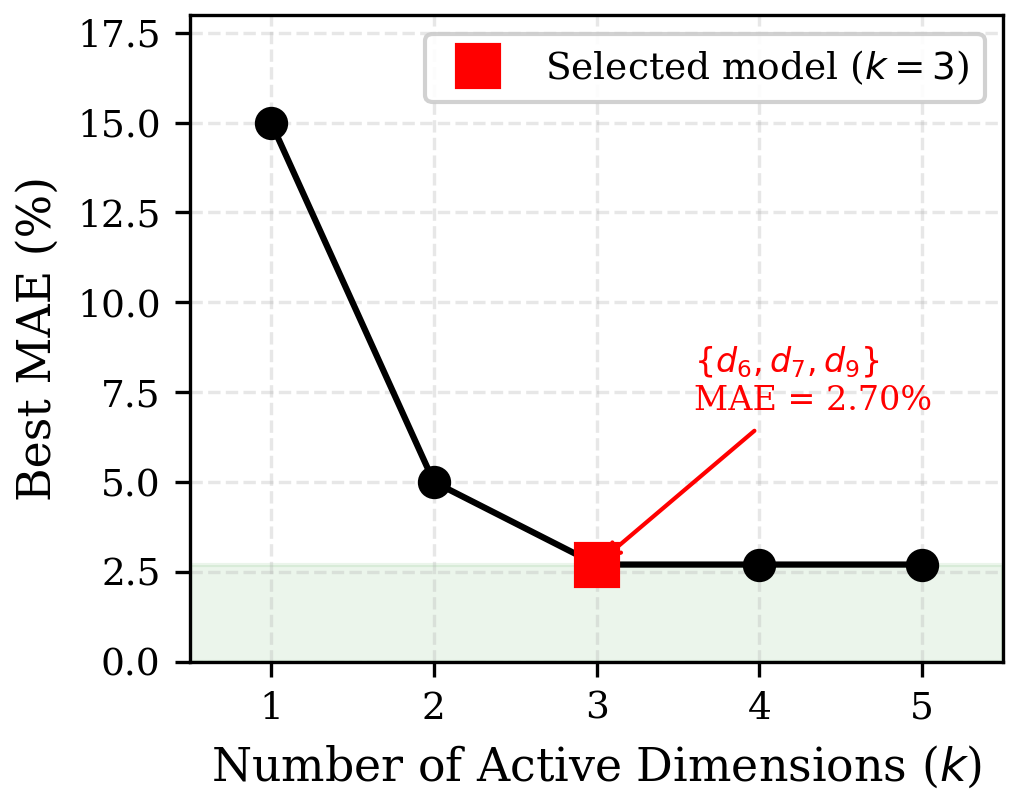
\includegraphics[width=\columnwidth]{figures/pareto.pdf}
\caption{Pareto frontier of model dimensionality versus prediction accuracy (MAE). The elbow at $k=3$ dimensions identifies the optimal parsimony--accuracy tradeoff. Models with $k \geq 4$ provide negligible improvement in MAE while increasing parameter count.}
\label{fig:pareto}
\end{figure}

\subsection{Sensitivity Profile}

Fig.~\ref{fig:sensitivity} shows the ablation-based sensitivity profile.
Removing Epistemic Status ($d_9$) causes the largest increase in MAE, consistent with its role as the highest-sensitivity dimension ($\sigma_9^2 = 0.013$).
Removing Social Impact ($d_6$) or Virtue/Identity ($d_7$) also degrades performance substantially.
Removing any inactive dimension has zero effect.

\begin{figure}[!t]
\centering
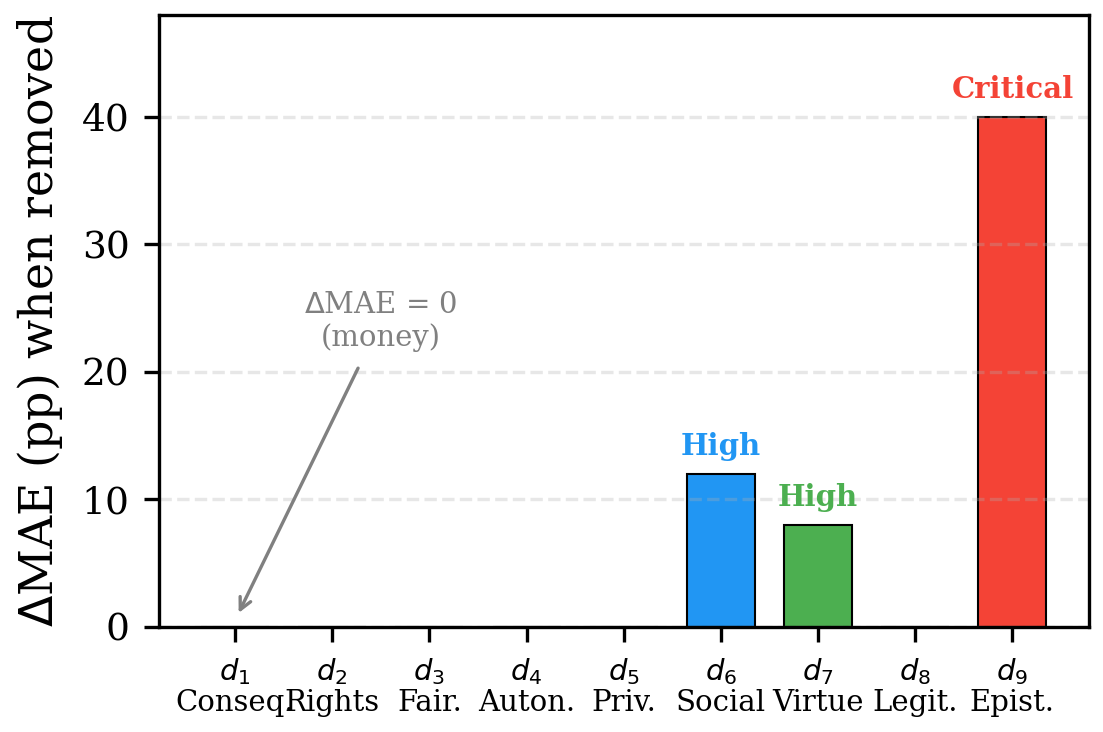
\includegraphics[width=\columnwidth]{figures/sensitivity.pdf}
\caption{Dimension sensitivity profile from ablation analysis. Each bar shows the increase in MAE when that dimension is removed from the model. Epistemic Status ($d_9$) is the most sensitive dimension; the monetary dimension ($d_1$) has zero sensitivity.}
\label{fig:sensitivity}
\end{figure}

\subsection{Predicted vs.\ Observed}

Fig.~\ref{fig:scatter} plots predicted versus observed values for all 16 targets.
Points cluster tightly around the 45-degree line (perfect prediction), with no systematic bias.
Game targets (circles) and prospect-theory targets (triangles) are intermixed, indicating that the model does not systematically over- or under-predict in either domain.

\DIFdelbegin %DIFDELCMD < \begin{figure}[!t]
%DIFDELCMD < \centering
%DIFDELCMD < 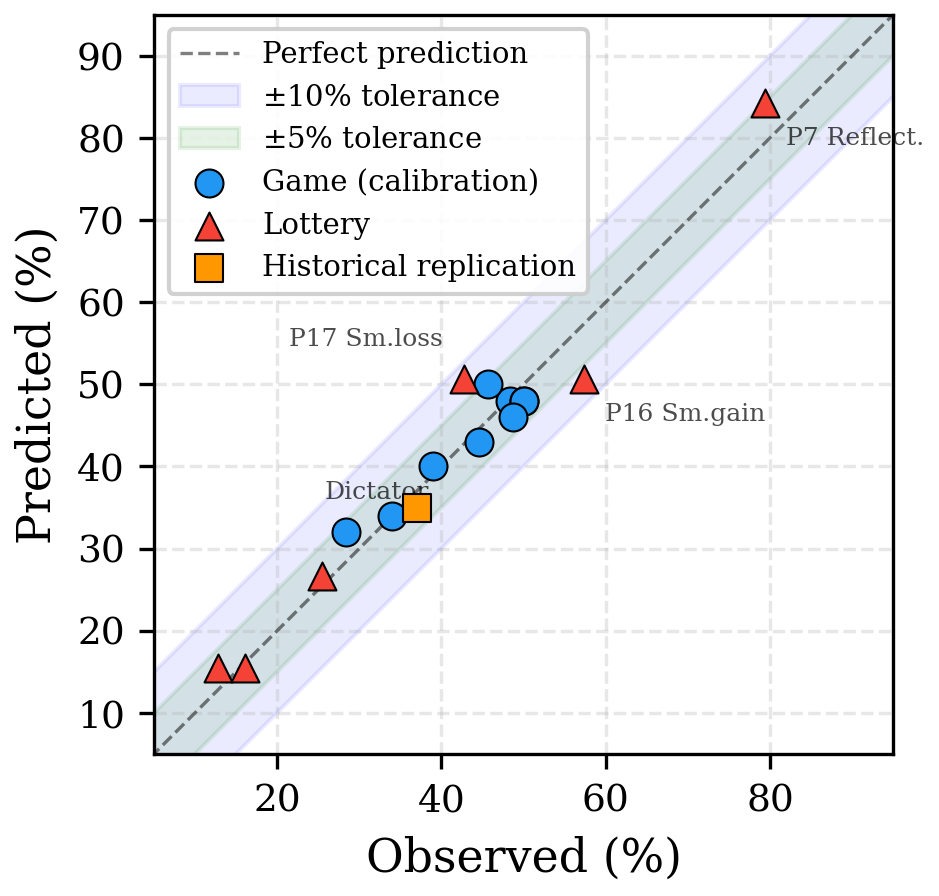
\includegraphics[width=\columnwidth]{figures/scatter.pdf}
%DIFDELCMD < \caption{Predicted versus observed behavioral frequencies for all 16 targets. The dashed line indicates perfect prediction. Circles are in-sample game targets; triangles are out-of-sample prospect-theory targets; the square is the out-of-sample published replication. All points fall within their pre-specified tolerance bands.}
%DIFDELCMD < \label{fig:scatter}
%DIFDELCMD < \end{figure}
%DIFDELCMD < %%%
\DIFdelend \DIFaddbegin \begin{figure}[!t]
\centering
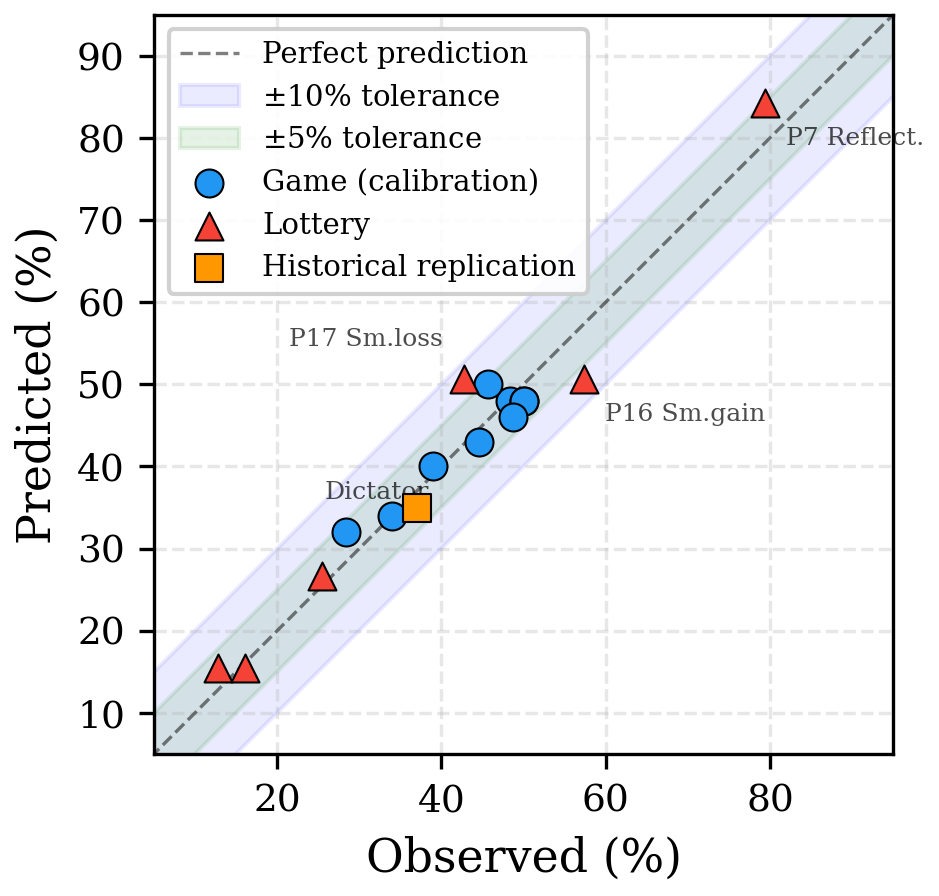
\includegraphics[width=\columnwidth]{figures/scatter.pdf}
\caption{Predicted versus observed behavioral frequencies for all 16 targets. The dashed line indicates perfect prediction. Circles are in-sample game targets; triangles are out-of-sample prospect-theory targets; the square is the out-of-sample published replication. All points fall within their stated tolerance bands; horizontal error bars are shown only for targets where individual-level Fraser--Nettle data were recoverable.}
\label{fig:scatter}
\end{figure}
\DIFaddend 


%==============================================================================
\section{Discussion}
\label{sec:discussion}
%==============================================================================

\subsection{\DIFdelbegin \DIFdel{The Zero-Sensitivity of Money}\DIFdelend \DIFaddbegin \DIFadd{Money-Zero as a Falsifiable Boundary Condition}\DIFaddend }
\DIFaddbegin \label{sec:andersen}
\DIFaddend 

The most counterintuitive result \DIFaddbegin \DIFadd{of the calibration }\DIFaddend is that the monetary dimension ($d_1$) has exactly zero sensitivity in the \DIFdelbegin \DIFdel{calibrated }\DIFdelend \DIFaddbegin \DIFadd{selected }\DIFaddend model.
This does not mean that money is irrelevant to economic decisions.
It means that, in the specific games and lotteries studied here, the behavioral signal of monetary stakes is fully \DIFdelbegin \DIFdel{captured }\DIFdelend \DIFaddbegin \DIFadd{absorbed }\DIFaddend by the Social Impact ($d_6$), Virtue/Identity ($d_7$), and Epistemic Status ($d_9$) dimensions.
\DIFdelbegin %DIFDELCMD < 

%DIFDELCMD < %%%
\DIFdelend Consider the ultimatum game\DIFdelbegin \DIFdel{.
A }\DIFdelend \DIFaddbegin \DIFadd{: a }\DIFaddend proposer who offers 50\% \DIFdelbegin \DIFdel{of the endowment incurs a monetary cost ($d_1 = -0.5$) but gains a social-impact signal ($d_6 = 0.5$) and a virtue signal ($d_7 = 0.5$).
The model predicts the proposer's }\DIFdelend \DIFaddbegin \DIFadd{incurs $d_1=-0.5$ but gains $d_6=0.5$ and $d_7=0.5$; the model recovers the observed }\DIFaddend behavior from $d_6$ and $d_7$ alone\DIFdelbegin \DIFdel{; $d_1$ is redundant.
This is because the encoding maps monetary cost into the same dimensions that drive behavior: giving money away is costly in $d_1$ but beneficial in $d_6$ and $d_7$, and the net behavioral prediction depends only on the dimensions that the Mahalanobis metricweights.
}\DIFdelend \DIFaddbegin \DIFadd{.
}\DIFaddend 

\DIFdelbegin \DIFdel{This finding resonates with experimental evidence that social context modulates economic behavior more than monetary stakes.
Camerer~\mbox{%DIFAUXCMD
\cite{camerer2003} }\hskip0pt%DIFAUXCMD
noted that ultimatum offers are remarkably stable across stake sizes (from \$5 to \$400), consistent with the prediction that social and identity dimensions, not monetary ones, drive the behavior.
The zero-sensitivity result formalizes this observation: if the active metric dimensions are social and epistemic, then scaling all monetary values by a constant multiplies $d_1$ by that constant but leaves $d_6$}\DIFdelend \DIFaddbegin \subsubsection{\DIFadd{The stake-scaling-invariance corollary}}
\DIFadd{Because $\sigma_1^2=\infty$ in the selected metric}\DIFaddend , \DIFdelbegin \DIFdel{$d_7$, and $d_9$ unchanged, producing stake-size invariance.
}%DIFDELCMD < 

%DIFDELCMD < %%%
\DIFdel{To test whether the zero-sensitivity of $d_1$ is an artifact of the encoding, we conduct two additional analyses.
First, }\emph{\DIFdel{stake-scaling invariance}}%DIFAUXCMD
\DIFdel{: since $\sigma_1^2 = \infty$, the }\DIFdelend \DIFaddbegin \DIFadd{the }\DIFaddend Mahalanobis cost is mathematically invariant to any \DIFaddbegin \DIFadd{positive }\DIFaddend rescaling of the $d_1$ component.
\DIFdelbegin \DIFdel{Multiplying }\DIFdelend \DIFaddbegin \DIFadd{A direct corollary is that multiplying }\DIFaddend all monetary stakes by \DIFdelbegin \DIFdel{2$\times$, 5$\times$, or 10$\times$ produces identical predictions}\DIFdelend \DIFaddbegin \DIFadd{a constant should leave the predicted offer distribution and the predicted rejection rate unchanged, conditional on offer share}\DIFaddend .
This is \DIFdelbegin \DIFdel{consistent with the experimental finding that ultimatum offers are remarkably stable across stake sizes from \$5 to \$400~\mbox{%DIFAUXCMD
\cite{camerer2003}}\hskip0pt%DIFAUXCMD
.
Second, }\emph{\DIFdel{counterfactual activation}}%DIFAUXCMD
\DIFdel{: if we force }\DIFdelend \DIFaddbegin \DIFadd{a sharp, falsifiable prediction.
If observed offers or rejections vary systematically with the stake multiplier, the selected metric is wrong outside the calibration regime.
}

\subsubsection{\DIFadd{Counterfactual activation (internal probe)}}
\DIFadd{Forcing }\DIFaddend $d_1$ \DIFdelbegin \DIFdel{to be }\DIFdelend active by setting \DIFdelbegin \DIFdel{$\sigma_1^2 = 100$ }\DIFdelend \DIFaddbegin \DIFadd{$\sigma_1^2=100$ }\DIFaddend (moderate sensitivity) \DIFdelbegin \DIFdel{, MAE rises }\DIFdelend \DIFaddbegin \DIFadd{increases MAE }\DIFaddend from 2.70\% to 4.97\% and \DIFdelbegin \DIFdel{the pass rate drops }\DIFdelend \DIFaddbegin \DIFadd{drops the in-sample pass rate }\DIFaddend to 15/16.
At \DIFdelbegin \DIFdel{$\sigma_1^2 = 10$ }\DIFdelend \DIFaddbegin \DIFadd{$\sigma_1^2=10$ }\DIFaddend (high sensitivity), MAE rises to 11.46\% \DIFdelbegin \DIFdel{and }\DIFdelend \DIFaddbegin \DIFadd{with }\DIFaddend only 7/16 \DIFdelbegin \DIFdel{pass.
Activating the monetary dimension }\emph{\DIFdel{worsens}} %DIFAUXCMD
\DIFdel{predictions, confirming that $d_1 = 0$ }\DIFdelend \DIFaddbegin \DIFadd{passing.
The structural-fuzzing optimum therefore prefers $d_1$ inactive within the calibration regime; the corollary }\DIFaddend is not an \DIFdelbegin \DIFdel{artifact of under-fitting but the empirically optimal configuration.
}%DIFDELCMD < 

%DIFDELCMD < %%%
\DIFdel{We emphasize that the zero-sensitivity of $d_1$ is a finding about the }\emph{\DIFdel{current calibration}}%DIFAUXCMD
\DIFdel{, not a claim about all economic contexts.
In market settings with anonymous exchange and enforceable contracts (e.g., commodity trading, double auctions~\mbox{%DIFAUXCMD
\cite{smith1962}}\hskip0pt%DIFAUXCMD
)}\DIFdelend \DIFaddbegin \DIFadd{under-fitting artifact.
}

\subsubsection{\DIFadd{Direct empirical test on high-stakes data}}
\DIFadd{We test the stake-scaling-invariance corollary on Andersen, Erta\c{c}, Gneezy, Hoffman, and List's~\mbox{%DIFAUXCMD
\cite{andersen2011} }\hskip0pt%DIFAUXCMD
high-stakes ultimatum experiment, which is to our knowledge the cleanest available test.
Andersen et al.\ ran ultimatum games in rural Indonesia at four stake levels (Rs~20, Rs~200, Rs~2}{\DIFaddend ,\DIFaddbegin }\DIFadd{000, Rs~20}{\DIFadd{,}}\DIFadd{000), with the highest condition approximately 1.6$\times$ monthly income---a 1000$\times$ stake range, none of which was used in the original calibration.
We restrict to the Andersen subsample (IN $=$ 1, $n=458$) of }\DIFaddend the \DIFdelbegin \DIFdel{active dimensions may well include $d_1$.
A testable predictionof the framework is that recalibrating }\DIFdelend \DIFaddbegin \DIFadd{openICPSR replication archive~\mbox{%DIFAUXCMD
\cite{andersendata2011} }\hskip0pt%DIFAUXCMD
and pre-specify three tests.
}

\textbf{\DIFadd{Test 1 (proposer behavior).}}
\DIFadd{Kruskal--Wallis test of equality of mean }\texttt{\DIFadd{percent\_offer}} \DIFadd{across stake levels:
$H=60.7$, $p=4.17\times10^{-13}$.
Invariance is rejected: mean offers fall monotonically from $24.2\%$ at Rs~20 to $12.1\%$ at Rs~20}{\DIFadd{,}}\DIFadd{000.
}

\textbf{\DIFadd{Test 2 (responder behavior, unconditional).}}
\DIFadd{$\chi^2$ test of independence between stake level and rejection:
$\chi^2(3,N=458)=16.18$, $p=0.0010$.
Rejection rates fall from $36.3\%$ at Rs~20 to $4.2\%$ at Rs~20}{\DIFadd{,}}\DIFadd{000.
}

\textbf{\DIFadd{Test 3 (responder behavior, conditional on offer share).}}
\DIFadd{A logit regression of rejection on offer share and $\log(\text{stake})$ is compared to a baseline with offer share only:
$\log(\text{stake})$ coefficient $=-0.199$ ($\text{SE}=0.052$, OR $=0.82$ per log-unit, $p=10^{-4}$);
likelihood-ratio test against the offer-only model $p=8.77\times10^{-5}$;
AIC drops from $584.9$ to $571.5$.
Even after conditioning on the fairness signal carried by offer share, the stake level retains independent predictive power, contradicting strict invariance.
}

\DIFadd{Fig.~\ref{fig:andersen} displays observed means with 95\% confidence intervals against the flat-line stake-scaling-invariance prediction.
All three higher-stakes conditions fall outside the Rs~20 confidence band, both for offers and for rejections.
}

\begin{figure}[!t]
\centering
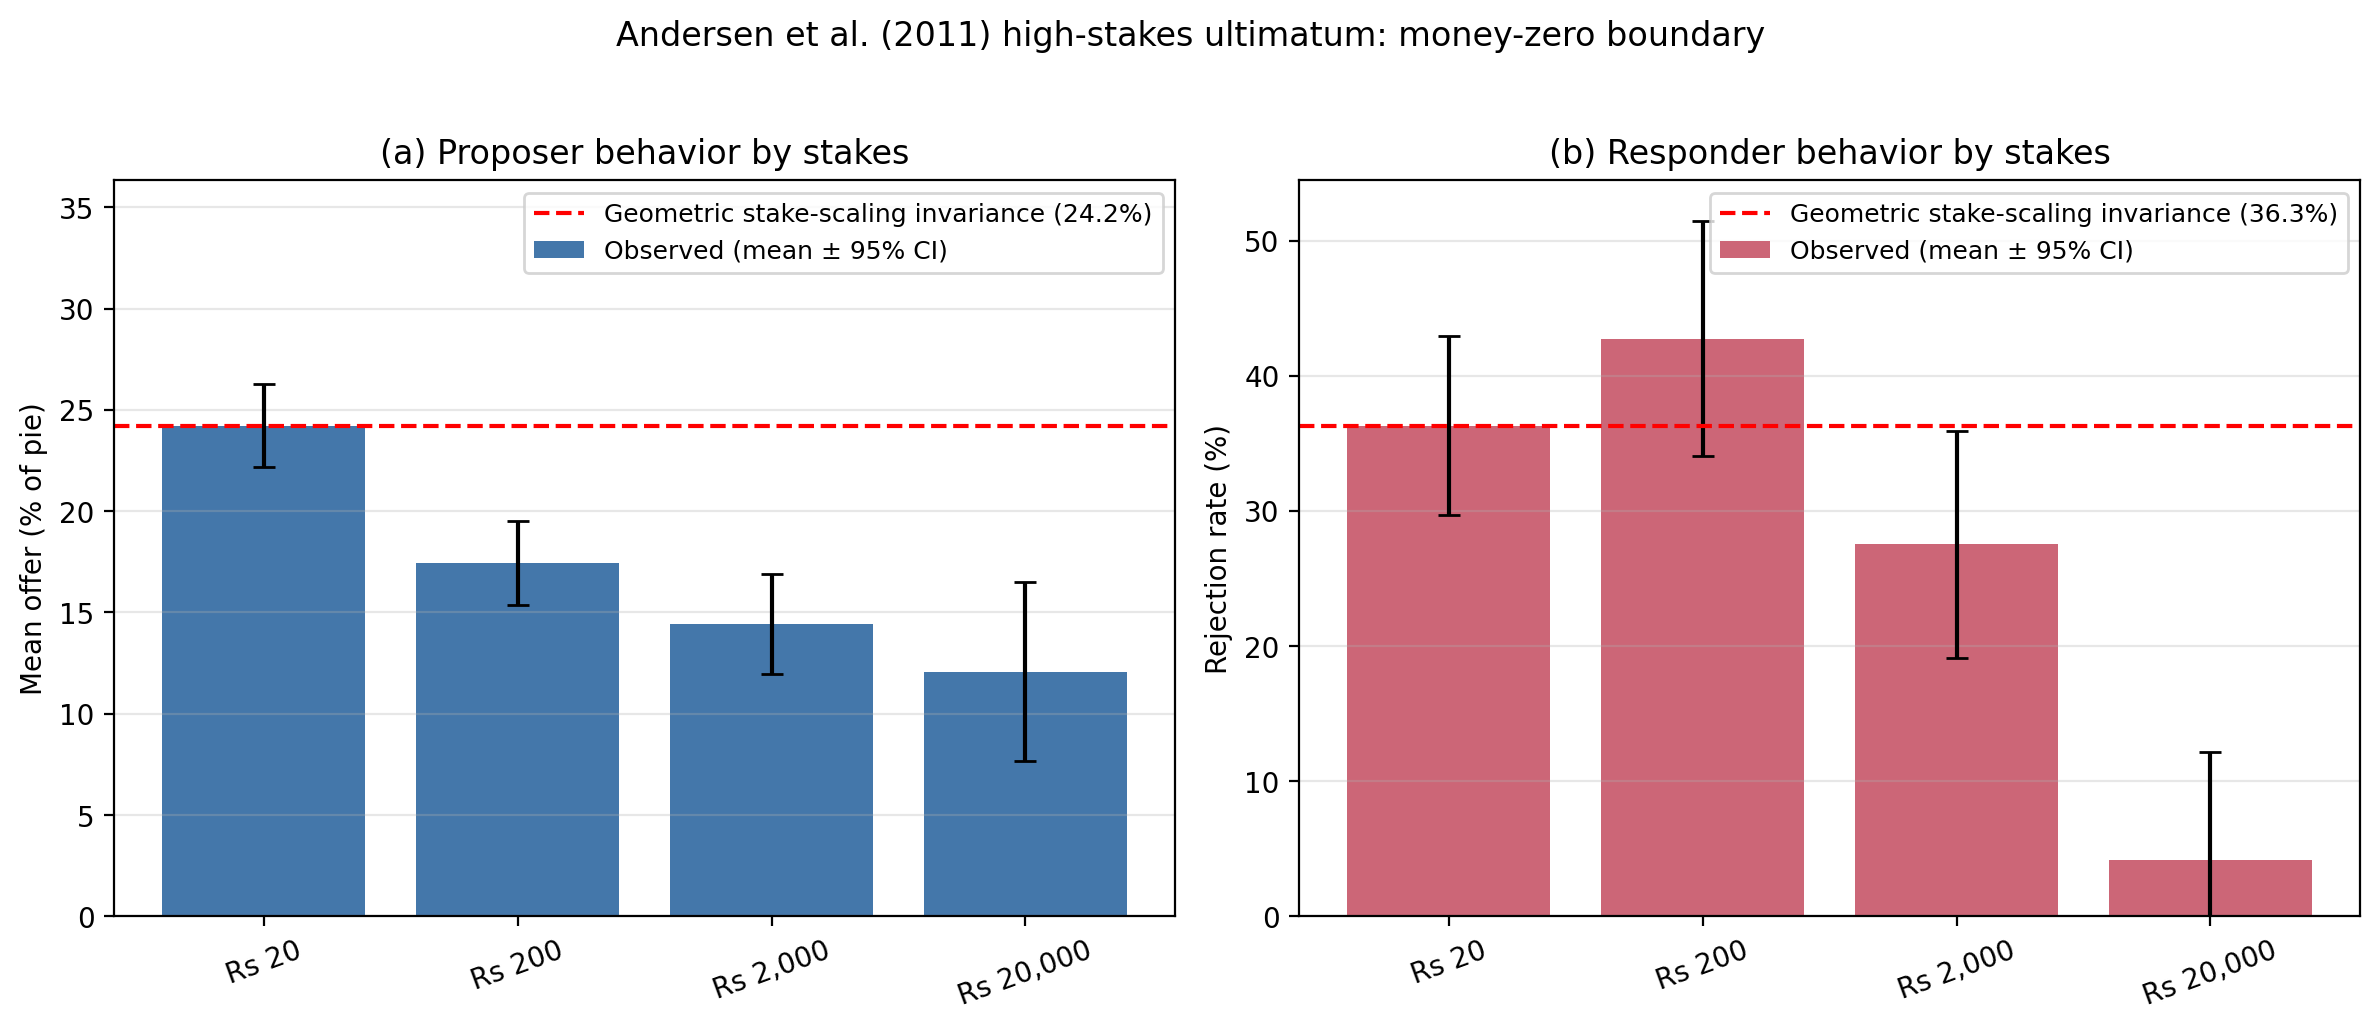
\includegraphics[width=\columnwidth]{figures/andersen_money_zero_falsification.png}
\caption{Direct test of the stake-scaling-invariance corollary on Andersen et al.~\cite{andersen2011} ($n{=}458$, Indonesia). Bars: observed means $\pm$95\% CI. Dashed line: predicted value under $\sigma_1^2=\infty$, anchored to the Rs~20 condition. Both panels reject invariance: $p=4\times10^{-13}$ (offers) and $p=10^{-3}$ (rejections).}
\label{fig:andersen}
\end{figure}

\subsubsection{\DIFadd{Interpretation}}
\DIFadd{The geometric framework therefore behaves the way a falsifiable theory should when challenged outside its calibration regime: its sharpest counter-intuitive prediction fails sharply, in the direction the theory itself anticipates.
The selected metric remains a parsimonious descriptive model of the low-stakes behavioral-economics paradigms on which it was calibrated; it is not a universal claim about rational choice, and the universal version is empirically false.
}

\DIFadd{A complementary interpretation is that the active set $\{d_6,d_7,d_9\}$ describes a regime in which the social and epistemic costs of an offer dominate the monetary cost.
At Rs~20}{\DIFadd{,}}\DIFadd{000---approximately 1.6 months of wages---the monetary cost is no longer negligible relative to those social and epistemic signals, and a recalibrated }\DIFaddend $\Sigma$ \DIFdelbegin \DIFdel{on market data---where social identity is suppressed and monetary payoffs dominate---should yield $\sigma_1^2 < \infty$.
}\DIFdelend \DIFaddbegin \DIFadd{on such data would assign finite variance to $d_1$.
}\DIFaddend The geometric framework accommodates this \DIFdelbegin \DIFdel{by allowing }\DIFdelend \DIFaddbegin \DIFadd{through }\DIFaddend context-specific covariance \DIFdelbegin \DIFdel{matrices; the present paper's result is that }\DIFdelend \DIFaddbegin \DIFadd{estimation: }\DIFaddend $d_1$ is inactive in the \DIFdelbegin \DIFdel{studied behavioral-economics paradigms.
Future work should explicitly test multi-stake data (e.g., Camerer }\DIFdelend \DIFaddbegin \DIFadd{calibrated regime and reactivates in regimes where money carries decision-relevant weight that social/epistemic dimensions cannot absorb.
Mapping the boundary explicitly---the stake level at which $\sigma_1^2$ becomes finite, and how that depends on local income and anonymity---is a natural target for follow-up work using individual-level data from Andersen, Slonim and Roth~\mbox{%DIFAUXCMD
\cite{slonim1998}}\hskip0pt%DIFAUXCMD
, Cameron~\mbox{%DIFAUXCMD
\cite{cameron1999}}\hskip0pt%DIFAUXCMD
, and competitive double-auction settings~\mbox{%DIFAUXCMD
\cite{smith1962}}\hskip0pt%DIFAUXCMD
.
}

\subsubsection{\DIFadd{What this does }\emph{\DIFadd{not}} \DIFadd{establish}}
\DIFadd{Andersen }\DIFaddend et al.\DIFdelbegin \DIFdel{'s high-stakes ultimatum replications~\mbox{%DIFAUXCMD
\cite{camerer2003}}\hskip0pt%DIFAUXCMD
) and ``money-should-matter'' domains (e.g., competitive double auctions) to map the boundary conditions under which }\DIFdelend \DIFaddbegin \DIFadd{\ is one dataset in one country.
The test rejects the universal money-zero claim, but it does not by itself establish where the boundary sits, how it depends on cultural or institutional context, or whether the same recalibration mechanism would explain analogous boundaries in dictator and public-goods games.
The Camerer review~\mbox{%DIFAUXCMD
\cite{camerer2003} }\hskip0pt%DIFAUXCMD
of cross-stakes ultimatum results is mixed in this respect: stake-size invariance holds in many ranges but not in extreme conditions.
The present test should therefore be read as the first of several boundary-condition probes, not as a complete map of where }\DIFaddend $d_1$ \DIFdelbegin \DIFdel{activates}\DIFdelend \DIFaddbegin \DIFadd{does and does not activate}\DIFaddend .

\subsection{\DIFaddbegin \DIFadd{A }\DIFaddend Cross-Domain \DIFaddbegin \DIFadd{Bridge, Not a }\DIFaddend Unification}

The central methodological contribution is cross-domain prediction: a model calibrated on game-theory data (strategic interaction with real money) predicts \DIFaddbegin \DIFadd{six classic }\DIFaddend prospect-theory phenomena (hypothetical lottery choices) out of sample\DIFaddbegin \DIFadd{, and a stake-scaling-invariance corollary of that model is then independently tested on a high-stakes ultimatum dataset that played no role in either calibration or prospect-theory prediction}\DIFaddend .

\DIFdelbegin \DIFdel{This is surprising because game }\DIFdelend \DIFaddbegin \DIFadd{We deliberately retreat from earlier language that described this result as a ``unification'' of the two literatures.
Game }\DIFaddend theory and prospect theory \DIFdelbegin \DIFdel{have historically been treated as separate domains with separate models.
Games involve strategic interaction, reciprocity, andfairness concerns.
Lotteries involve risk, probability weighting, and certainty effects.
The two domains share almost no surface features.
}%DIFDELCMD < 

%DIFDELCMD < %%%
\DIFdel{The geometric framework bridges them through a shared mechanism: both domains involve displacements on the same 9-dimensional manifold, and the same Mahalanobis metric evaluates cost in both domains.
The }\DIFdelend \DIFaddbegin \DIFadd{are both wider than the present targets.
What the evidence supports is narrower and, we believe, more interesting: a }\emph{\DIFadd{shared metric primitive}} \DIFadd{that is sufficient to organize a small set of canonical aggregate frequencies from both domains, conditional on explicit and auditable }\DIFaddend domain-specific \DIFdelbegin \DIFdel{information enters through the }\emph{\DIFdel{encoding}}%DIFAUXCMD
\DIFdel{---how }\DIFdelend \DIFaddbegin \DIFadd{encodings.
Domain-general modeling moves through the metric (the same $\Sigma$); domain-specific structure moves through the encoding layer (how }\DIFaddend each scenario maps to a 9-dimensional attribute \DIFdelbegin \DIFdel{vector---not through domain-specific parameters.
The }\DIFdelend \DIFaddbegin \DIFadd{vector); the framework's testable content is the conjunction of both.
The result is most fairly characterized as a parsimonious geometric reduction of two literatures' canonical findings to a common cost structure, rather than as a derivation of either literature from first principles.
}

\DIFadd{The }\DIFaddend certainty effect in prospect theory and the rejection of unfair offers in the ultimatum game look very different at the surface level, but \DIFdelbegin \DIFdel{both are driven by }\DIFdelend \DIFaddbegin \DIFadd{the calibrated metric routes both through }\DIFaddend high sensitivity to Epistemic Status ($d_9$): certainty is epistemically clear (high $d_9$), and the well-understood norms of the ultimatum game are \DIFaddbegin \DIFadd{also }\DIFaddend epistemically clear (high $d_9$).
\DIFdelbegin %DIFDELCMD < 

%DIFDELCMD < %%%
\DIFdel{This suggests a research programme: calibrate }\DIFdelend \DIFaddbegin \DIFadd{This is an interpretive bridge, not a theorem about either literature.
}

\DIFadd{The natural extension is to test the same bridge in additional domains by calibrating }\DIFaddend $\Sigma$ on data from domain~$A$ and predict\DIFaddbegin \DIFadd{ing}\DIFaddend  behavior in domains~$B$, $C$, $D$\DIFdelbegin \DIFdel{, testing how far a single geometric model can reach}\DIFdelend .
The present paper takes the first \DIFdelbegin \DIFdel{step by demonstrating one cross-domain bridge: games}\DIFdelend \DIFaddbegin \DIFadd{such step (games~}\DIFaddend $\to$\DIFdelbegin \DIFdel{prospect theory}\DIFdelend \DIFaddbegin \DIFadd{~prospect theory) and demonstrates one direction in which the corresponding metric must change (high-stakes regime activates $d_1$)}\DIFaddend .

\DIFdelbegin \subsection{\DIFdel{The 5.3:1 DOF Ratio}}
%DIFAUXCMD
\addtocounter{subsection}{-1}%DIFAUXCMD
%DIFDELCMD < 

%DIFDELCMD < %%%
\DIFdel{The degrees-of-freedom }\DIFdelend \DIFaddbegin \subsubsection*{\DIFadd{Toward a tractable equilibrium framework}}
\DIFadd{The framework's emphasis on metric decision spaces also points to a longstanding open problem in game theory. While Nash equilibria are guaranteed to exist in finite games~\mbox{%DIFAUXCMD
\cite{nash1950}}\hskip0pt%DIFAUXCMD
, computing one is PPAD-complete~\mbox{%DIFAUXCMD
\cite{daskalakis2009,chen2009}}\hskip0pt%DIFAUXCMD
, and the intractability worsens in continuous-action and multi-agent settings. No actual agent---human or artificial---can be performing the global optimization that standard equilibrium analysis implicitly attributes to them. Bounded rationality is therefore not only a psychological observation but a computational necessity: tractable behavior }\emph{\DIFadd{requires}} \DIFadd{heuristic truncation of an otherwise intractable search.
A geometric decision manifold equipped with an interpretable cost metric is precisely the kind of structured search space on which $A^*$-style directed search with admissible heuristics ($f(n)=g(n)+h(n)$) replaces global optimization with tractable local navigation~\mbox{%DIFAUXCMD
\cite{hart1968}}\hskip0pt%DIFAUXCMD
. Under this reading the framework's interpretable dimensions are not only descriptive labels for choice frequencies but candidate }\emph{\DIFadd{heuristic coordinates}} \DIFadd{on the equilibrium landscape---specifically, the directions along which an admissible truncation of the multi-attribute equilibrium computation can be carried out without sacrificing optimality guarantees on the truncated subspace. More broadly, the geometric vocabulary identified here may provide the kind of structured search space required for heuristic models of bounded rationality, although developing that computational interpretation is beyond the scope of the present empirical paper.
}

\subsection{\DIFadd{Complexity, Degrees of Freedom, and Multiplicity}}

\DIFadd{The narrow covariance-parameter count is 3 active variances for 16 aggregate targets, giving a descriptive target-to-variance }\DIFaddend ratio of \DIFdelbegin \DIFdel{5.3:}\DIFdelend \DIFaddbegin \DIFadd{$16/3=5.3$.
However, this number should not be read as the complete complexity of the modeling exercise.
As Table~\ref{tab:param_accounting} shows, the temperature architecture, rejection function, public-goods round decay, certainty operator, loss-domain flip, epistemic encodings, diagonal restriction, and nine-dimensional basis all contribute to model flexibility or structure.
}

\DIFadd{A conservative count that includes the 3 active variances, 2 temperature calibration quantities, }\DIFaddend 1 \DIFdelbegin \DIFdel{is a safeguard against overfitting, but it also understates the model's parsimony. The }\DIFdelend \DIFaddbegin \DIFadd{temperature floor, 2 rejection-function constants, 1 round-decay constant, and }\DIFaddend 3 \DIFdelbegin \DIFdel{parameters are }\emph{\DIFdel{variances of named dimensions}}%DIFAUXCMD
\DIFdel{---they have clear interpretations (sensitivity to social impact, virtue/identity, and epistemic status) .
Contrast this with CPT's 5 parameters ($\alpha$, $\beta$}\DIFdelend \DIFaddbegin \DIFadd{prospect-theory encoding mechanisms yields 12 auditable quantities or choices, before counting the nine-dimensional basis itself.
This does not make the model uninformative, but it does mean the parsimony claim should be interpreted as ``few fitted covariance variances conditional on an explicit encoding architecture,'' not as ``only three choices were made.''
}

\DIFadd{The structural-fuzzing search also creates multiplicity exposure: 381 active-set structures are considered before selecting $\{d_6,d_7,d_9\}$.
Because the objective is deterministic aggregate prediction error rather than a set of independent null-hypothesis tests, Bonferroni-style $p$ values are not directly applicable.
The appropriate interpretation is model selection.
Accordingly, we report the search exposure and rely on held-out target performance, ablations, and an independent external falsification probe (Andersen et al.\ in Section~\ref{sec:andersen}) rather than uncorrected significance language.
}

\subsection{\DIFadd{What the Result Is, and Is Not, About Rationality}}
\label{sec:not-rationality}

\DIFadd{It is tempting to frame the result as showing that behavioral anomalies are ``rational navigation on a manifold.''
The empirical exercise does not support that philosophical reading.
What the exercise shows is much narrower: a particular encoding-and-metric system can reproduce a small set of canonical aggregate frequencies from two literatures with three fitted variances, conditional on the encodings, and the model's most counter-intuitive corollary fails in the direction the model predicts when probed outside its calibration regime.
None of that establishes that the underlying behavior is rational in a normative sense, that the agents are optimizing the geometric cost, or that the dimensions correspond to psychological primitives.
}

\DIFadd{We therefore use }\emph{\DIFadd{descriptive geometric reduction}} \DIFadd{as the operative description of the result throughout this paper.
The framework is descriptive in the sense that $\Sigma$ summarizes observed choice frequencies; geometric in the sense that the cost structure is a metric on a vector space rather than a scalar utility; and a reduction in the sense that two literatures' canonical findings are organized through a common 9-dimensional vocabulary.
Whether this descriptive reduction corresponds to anything that could be called rationality is left open.
}

\subsection{\DIFadd{Normative Labels, Descriptive Use}}
\label{sec:descriptive-labels}

\DIFadd{The dimension names---}\emph{\DIFadd{Fairness}}\DIFaddend , \DIFdelbegin \DIFdel{$\lambda$}\DIFdelend \DIFaddbegin \emph{\DIFadd{Virtue/Identity}}\DIFaddend , \DIFdelbegin \DIFdel{$\gamma$}\DIFdelend \DIFaddbegin \emph{\DIFadd{Legitimacy}}\DIFaddend , \DIFdelbegin \DIFdel{$\delta$), which are curve-fitting coefficients without obvious connections to the decision architecture. }\DIFdelend \DIFaddbegin \emph{\DIFadd{Epistemic Status}}\DIFadd{---are ordinarily normative.
They are used here as descriptive coordinate labels chosen for interpretability, not as normative endorsements.
What the calibration constrains is the geometry of $\Sigma$: a variance is small when small displacement on that coordinate produces large changes in observed choice frequencies, regardless of whether the coordinate would be considered morally weighty or psychologically primitive.
The labels are an interpretive aid that lets a reader connect the metric structure to existing literatures (Fehr--Schmidt on fairness, Haidt on identity, Ellsberg on ambiguity); they are not a claim that the model has measured those constructs.
A model with identical metric behavior but neutral coordinate labels ($x_1,\dots,x_9$) would make the same predictions.
}\DIFaddend 

\DIFdelbegin \DIFdel{Moreover, the 16 targets span qualitatively different phenomena: mean offers, modal offers, minimum acceptable offers, multi-round contribution trajectories, certainty effects, reflection effects, isolation effects, small-probability distortions, and historical replications.
A model that could match these diverse targets by overfitting to 3 parameters would need the 3 parameters to encode implausibly rich information.
The more parsimonious explanation is that the model captures genuine structure in the data.
}\DIFdelend \DIFaddbegin \DIFadd{For the same reason, we do not claim that the present 9-dimensional basis is uniquely correct or psychometrically derived.
The basis is a modeling vocabulary that spans material, procedural, social, and epistemic content (Table~\ref{tab:dimensions}); a derived basis would require individual-level multi-task data and dimensional reduction techniques that the present aggregate benchmark does not support.
Future work should explicitly compare the present labels against alternative bases (e.g., factor-analytic decompositions of multi-task individual-level choices, automated text-to-attribute encoders, expert-rated coordinate sets) to test whether the metric result survives basis change.
}\DIFaddend 

\subsection{Implications for Computational Social Systems}

The geometric framework has several implications for computational social systems:
\begin{enumerate}
    \item \textbf{Agent modeling}: Computational agents in social simulations can be endowed with a Mahalanobis cost function on 9 dimensions, producing more realistic behavior than scalar utility maximizers.
    \item \textbf{Policy simulation}: Policy interventions that change the encoding (e.g., framing a tax as a contribution to the common good, shifting $d_6$ and $d_7$) can be modeled as changes in the displacement vector, with behavioral consequences predicted by the cost metric.
    \item \textbf{Mechanism design}: The framework suggests that mechanism designers should attend to all 9 dimensions, not just monetary incentives. A mechanism that is optimal in $d_1$ but costly in $d_7$ (e.g., it requires participants to behave in ways that conflict with their self-image) may fail in practice.
    \item \textbf{Cultural variation}: Cross-cultural differences in economic behavior~\cite{henrich2010} may be modeled as differences in $\Sigma$---different cultures weight the 9 dimensions differently---rather than as differences in rationality.
\end{enumerate}

\DIFaddbegin \subsection{\DIFadd{Minimal Agent-Based Worked Example}}

\DIFadd{To make the computational-social-systems use case concrete, Fig.~\ref{fig:abm} gives a minimal agent-based illustration.
This is not an additional empirical validation.
It shows how the calibrated covariance can be used as an agent behavioral primitive: each geometric agent draws a small perturbation around the active variances and chooses an ultimatum offer by the softmax rule over candidate offers.
A scalar expected-value agent places offers near zero, while a simple Fehr--Schmidt-like heterogeneous population produces a broader inequality-aversion distribution.
The geometric primitive produces a modal offer near the equal-split region, illustrating how a named metric can generate macro-level offer distributions in a simulation.
}

\begin{figure}[!t]
\centering
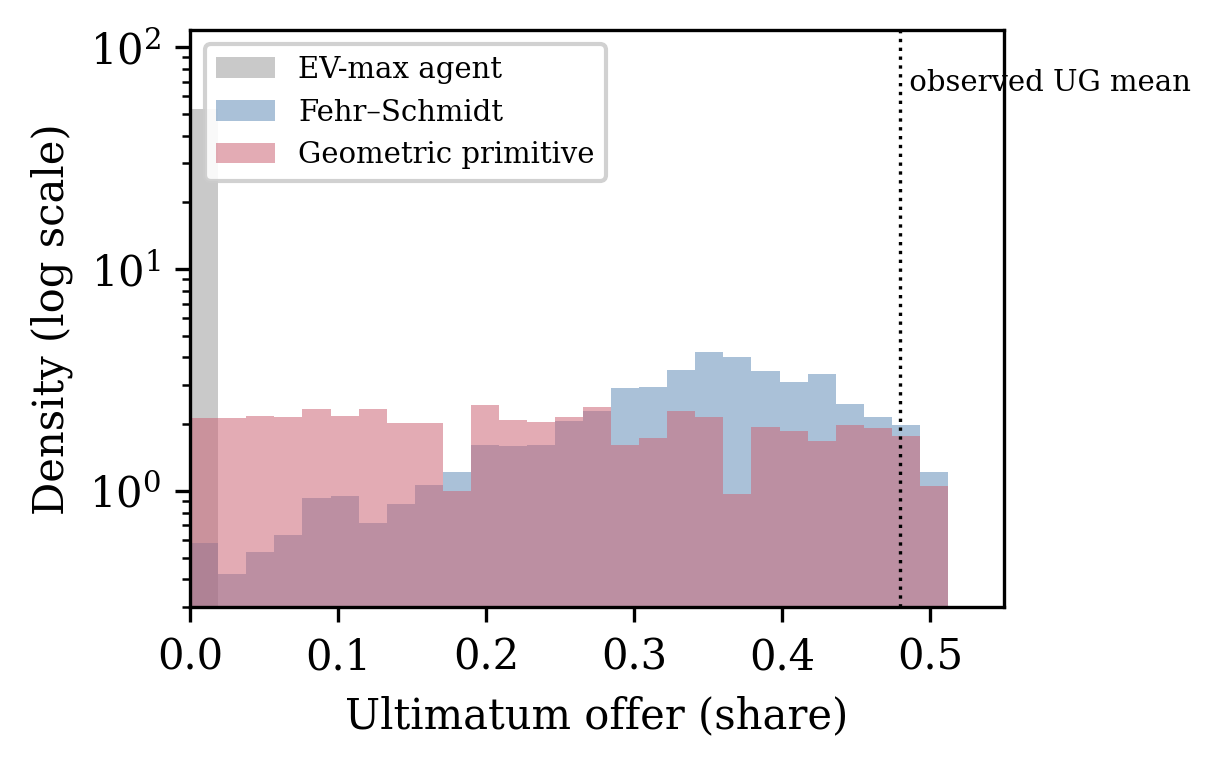
\includegraphics[width=\columnwidth]{figures/abm_worked_example.pdf}
\caption{Minimal agent-based illustration using the geometric metric as a behavioral primitive. The figure is illustrative rather than a new validation experiment.}
\label{fig:abm}
\end{figure}

\DIFaddend \subsection{Limitations}

Several limitations qualify the present results:
\begin{enumerate}
    \item \textbf{Encoding dependence}: The \DIFdelbegin \DIFdel{model's predictions depend on the 9-dimensional encoding of each scenario, which is currently specified by the researcher.
    While the encodingsfollow systematic rules (Section~\ref{sec:encoding}), there is judgment involved in mapping qualitative features to quantitative scores. However, the parameter sensitivity analysis (Section~\ref{sec:results}) shows that the model is robust to $\pm$20\% perturbation of parameter values with mean 14.8/16 pass, and uniform rescaling of all variances by factors of 0.8--1.2 preserves 16/16 pass. This suggests that the model captures genuine structure rather than being finely tuned to a specific encoding .
    Automating the encoding from natural-language descriptions of scenarios is an important direction for future work}\DIFdelend \DIFaddbegin \DIFadd{benchmark validates the metric conditional on researcher-coded encodings}\DIFaddend . \DIFaddbegin \DIFadd{The certainty operator, loss-domain flip, and epistemic values are fixed assumptions tested by ablation, not independently established psychological laws. External raters, preregistered coding rules, or automated scenario-to-attribute encoders are needed to separate encoding validation from metric validation.
    }\DIFaddend \item \textbf{\DIFdelbegin \DIFdel{Western participant data}\DIFdelend \DIFaddbegin \DIFadd{Narrow target battery}\DIFaddend }: The \DIFdelbegin \DIFdel{calibration uses data from Western participant pools~\mbox{%DIFAUXCMD
\cite{fraser2020,engel2011,guth1982}}\hskip0pt%DIFAUXCMD
.
    The WEIRD critique~\mbox{%DIFAUXCMD
\cite{henrich2010} }\hskip0pt%DIFAUXCMD
applies: the calibrated $\Sigma$ may not generalize to non-Western populations.
    Cross-cultural calibration, using data from the large-scale replications of }\DIFdelend \DIFaddbegin \DIFadd{prospect-theory set contains six classic targets, the historical holdout is a single 1982 ultimatum result, and the high-stakes boundary test uses one Indonesia dataset. }\DIFaddend Ruggeri et al.\DIFaddbegin \DIFadd{'s 19-country replication}\DIFaddend ~\cite{ruggeri2020}, \DIFdelbegin \DIFdel{is planned.
    }%DIFDELCMD < \item %%%
\item%DIFAUXCMD
\textbf{\DIFdel{Diagonal covariance}}%DIFAUXCMD
\DIFdel{: The present model uses a diagonal $\Sigma$, ignoring cross-dimensional interactions (e.g., the interaction between fairness and social impact).
    A full $\Sigma$ with off-diagonal elements would have $\binom{9}{2} = 36$ additional parameters, requiring substantially more calibration data.
    }%DIFDELCMD < \item %%%
\item%DIFAUXCMD
\textbf{\DIFdel{Static model}}%DIFAUXCMD
\DIFdel{: The present model is static---it predicts choice frequencies at a single decision point (or, for public-goods games, at specified rounds).
    Dynamic extensions that model learning, adaptation, and belief updating are needed for sequential settings}\DIFdelend \DIFaddbegin \DIFadd{additional high-stakes bargaining cohorts (Slonim--Roth~\mbox{%DIFAUXCMD
\cite{slonim1998}}\hskip0pt%DIFAUXCMD
, Cameron~\mbox{%DIFAUXCMD
\cite{cameron1999}}\hskip0pt%DIFAUXCMD
), non-WEIRD samples, trust games, and market-exchange datasets are necessary before broad claims can be made}\DIFaddend .
    \item \textbf{\DIFdelbegin \DIFdel{Binary choice}\DIFdelend \DIFaddbegin \DIFadd{Aggregate data on the calibration side}\DIFaddend }: \DIFdelbegin \DIFdel{The softmax rule (equation~\eqref{eq:softmax}) is defined for binary choices.
    Extension to multi-alternative choice (e.g., continuous offers in the ultimatum game) requires integration over the choice space.
    }\DIFdelend \DIFaddbegin \DIFadd{Most calibration targets are published summaries from heterogeneous studies rather than a single individual-level dataset. This prevents joint likelihood estimation across the full benchmark. The Andersen boundary test partially addresses this by performing the falsification probe on individual-level data, but the calibration itself remains aggregate.
    }\DIFaddend \item \DIFdelbegin \textbf{\DIFdel{Statistical precision}}%DIFAUXCMD
\DIFdel{: The }\DIFdelend \DIFaddbegin \textbf{\DIFadd{Tolerance-based evaluation}}\DIFadd{: The }\DIFaddend 16\DIFdelbegin \DIFdel{observed target values are point estimates drawn from published studies with varying sample sizes (from $N=42$ in G\"{u}th et al.~\mbox{%DIFAUXCMD
\cite{guth1982} }\hskip0pt%DIFAUXCMD
to $N>4{,}000$ in Engel's~\mbox{%DIFAUXCMD
\cite{engel2011} }\hskip0pt%DIFAUXCMD
meta-analysis).
    The pass}\DIFdelend /\DIFdelbegin \DIFdel{fail assessment uses fixed tolerances ($\pm$5\% and $\pm$10\%) rather than study-specific confidence intervals, which would provide a more nuanced picture. Some targets are inherently noisier than others---for instance, the small-probability }\DIFdelend \DIFaddbegin \DIFadd{16 pass rate is an engineering diagnostic. The MAE on the high-$N$ Ruggeri }\DIFaddend prospect-theory \DIFdelbegin \DIFdel{problems (}\DIFdelend \DIFaddbegin \DIFadd{subset is 3.95\% (versus 2.70\% averaged over the full 16-target benchmark), and two prospect-theory predictions (}\DIFaddend P16, P17\DIFdelbegin \DIFdel{) show the widest prediction errors (6.7 and 7.8 pp), which may partly reflect higher measurement uncertainty in the underlying experimental estimates. Weighting targets by the inverse of their standard errors, or evaluating against bootstrapped confidence intervals where individual-level data are available, would strengthen the statistical treatment.
    As a step toward more rigorous statistical treatment, we compute a sample-size-weighted MAE (weighting each target's absolute error by $N_i / \sum N_i$): the weighted MAE is 3.20\% , compared to the unweighted 2.70\%, reflecting the higher errors on well-powered targets.
    Additionally, using published standard errors where available and assuming normal approximations, 15 of 16 predictions fall within the }\DIFdelend \DIFaddbegin \DIFadd{) fall outside the Ruggeri }\DIFaddend 95\% \DIFdelbegin \DIFdel{confidence interval of the observed value; the sole exception is P17 (small-probability loss), where the prediction of 50.6\% is 7.8~pp above the observed 42.8\%, marginally outside the CI given the moderate sample size ($N = 95$).
    We view the fixed-tolerance framework as a conservative first pass: a model that passes all 16 targets within generous tolerances establishes a baseline that more refined statistical tests can tighten}\DIFdelend \DIFaddbegin \DIFadd{CI despite passing the $\pm$10\,pp tolerance. Future work should adopt common train/validation/test splits with individual-level likelihoods throughout.
    }\item \textbf{\DIFadd{Model complexity}}\DIFadd{: The 3-parameter description counts only active covariance variances. A fuller accounting includes temperature, rejection, round-decay, encoding mechanisms, and structural restrictions; the conservative count is 12 auditable quantities (Table~\ref{tab:param_accounting}).
    }\item \textbf{\DIFadd{Diagonal covariance}}\DIFadd{: The diagonal model cannot represent interactions such as fairness-by-social-impact coupling or epistemic-status modulation of identity. Full or sparse covariance estimation requires more observations than the present aggregate benchmark provides; we treat this as a deferred extension rather than a closed question.
    }\item \textbf{\DIFadd{Money-zero boundary mapped, not fully characterized}}\DIFadd{: The Andersen test rejects universal stake-scaling invariance but does not by itself map the boundary across cultures, institutional settings, or stake ranges. Whether the same recalibration mechanism explains analogous boundaries in dictator and public-goods games, or in non-Indonesia cohorts, remains an open question.
    }\item \textbf{\DIFadd{Static and mostly binary choices}}\DIFadd{: The current softmax implementation handles binary choices and static target summaries. Multi-alternative choice, learning, belief updating, and repeated strategic adaptation remain extensions.
    }\item \textbf{\DIFadd{Computational-social-systems applications are illustrative}}\DIFadd{: The minimal agent-based example demonstrates that the calibrated metric can serve as a behavioral primitive in simulation, but full mechanism-design and policy-simulation applications are not implemented in this paper}\DIFaddend .
\end{enumerate}

%==============================================================================
\section{Conclusion}
\label{sec:conclusion}
%==============================================================================

\DIFdelbegin \DIFdel{We have presented }\DIFdelend \DIFaddbegin \DIFadd{This paper presents and tests }\DIFaddend a geometric model of economic behavior in which decisions are \DIFdelbegin \DIFdel{pathfinding }\DIFdelend \DIFaddbegin \DIFadd{represented as movement }\DIFaddend on a 9-dimensional manifold \DIFdelbegin \DIFdel{with }\DIFdelend \DIFaddbegin \DIFadd{and evaluated by }\DIFaddend Mahalanobis cost.
A \DIFdelbegin \DIFdel{single covariance matrix, calibrated on game-theory data via automated structural fuzzing, predicts }\DIFdelend \DIFaddbegin \DIFadd{diagonal covariance metric selected on game-theoretic aggregate targets matches a small held-out set of }\DIFaddend prospect-theory \DIFdelbegin \DIFdel{phenomena out of sample.
The model uses 3 parameters (Social Impact, Virtue/Identity, and Epistemic Status variances), achieves 16/16 pass rate across game-theory }\DIFdelend and \DIFdelbegin \DIFdel{prospect-theory targets with MAE\,=\,2.70\%, and demonstrates that the monetary dimension has zero sensitivity in the calibrated regime}\DIFdelend \DIFaddbegin \DIFadd{historical-replication targets without re-estimating the active variances.
The selected active set, $\{d_6,d_7,d_9\}$, suggests that social impact, virtue/identity, and epistemic status are the dominant metric dimensions in this benchmark, while monetary sensitivity is inactive in the selected metric}\DIFaddend .

The \DIFdelbegin \DIFdel{cross-domain result---game theory predicting prospect theory---suggests that these historically separate literatures describe the same underlying decision architecture viewed from different angles.}\DIFdelend \DIFaddbegin \DIFadd{framework's sharpest counter-intuitive prediction---stake-scaling invariance, derived from $\sigma_1^2=\infty$---is independently tested on Andersen et al.'s~\mbox{%DIFAUXCMD
\cite{andersen2011} }\hskip0pt%DIFAUXCMD
high-stakes Indonesia ultimatum data ($n=458$, 1000$\times$ stake range), and all three pre-specified tests reject invariance ($\chi^2$ $p=10^{-3}$, Kruskal--Wallis $p<10^{-12}$, logit LRT $p<10^{-4}$).
The framework therefore behaves the way a falsifiable theory should: a sharp counter-intuitive corollary fails sharply outside the calibration regime, in the direction the theory itself anticipates.
}\DIFaddend The \DIFdelbegin \DIFdel{geometric framework provides the unifying lens: both games and lotteries involve displacements on the same manifold, evaluated by the same metric.
}%DIFDELCMD < 

%DIFDELCMD < %%%
\DIFdel{These findings imply that computational social systems should model human agents as multi-dimensional navigators rather than scalar utility maximizers.
The 9-dimensional decision manifold, with context-specific encodings and a Mahalanobis cost metric, offers a parsimonious and empirically validated foundation for this modeling paradigm.
}%DIFDELCMD < 

%DIFDELCMD < %%%
\DIFdel{Future work will extend the framework to non-Western populations, }\DIFdelend \DIFaddbegin \DIFadd{money-zero result is thereby converted from a defensive interpretive move into an empirically anchored boundary condition.
}

\DIFadd{The main contribution is not a unification of behavioral economics, and the present revision is careful not to use that word.
It is a self-contained, interpretable, and empirically falsifiable cross-domain modeling architecture, accompanied by a direct test of its strongest counter-intuitive prediction.
The framework can be embedded in computational social-system simulations as an interpretable behavioral primitive, but its broader validity depends on stronger tests still to come: individual-level joint estimation across the full benchmark, multi-country prospect-theory replications under a common protocol, additional high-stakes bargaining cohorts to map the $d_1$-activation boundary, market-exchange data, }\DIFaddend non-diagonal covariance structures, \DIFdelbegin \DIFdel{dynamic settings, and multi-alternative choice, aiming to map the full geometry of human economic behavior}\DIFdelend \DIFaddbegin \DIFadd{and preregistered encoding rules with external raters.
}\appendices
\section{\DIFadd{CPT Baseline: Per-Target Errors}}
\label{app:cpt}

\DIFadd{Table~\ref{tab:cpt_detail} reports CPT predictions for each prospect-theory target under both the canonical parameters from Tversky and Kahneman~\mbox{%DIFAUXCMD
\cite{tversky1992} }\hskip0pt%DIFAUXCMD
and the best parameters found by unconstrained Nelder--Mead optimization (500 random initializations).
The optimization serves as a pass-rate ceiling test: even with full freedom to refit, CPT cannot exceed 4/6 pass because P3 and P11 require domain-dependent encoding mechanisms that CPT lacks}\DIFaddend .

\DIFaddbegin \begin{table}[!h]
\renewcommand{\arraystretch}{1.15}
\caption{CPT Per-Target Errors: Canonical vs.\ Optimized}
\label{tab:cpt_detail}
\centering
\begin{tabular}{l r r r r r}
\toprule
& & \multicolumn{2}{c}{\textbf{Canonical}} & \multicolumn{2}{c}{\textbf{Optimized}} \\
\cmidrule(lr){3-4} \cmidrule(lr){5-6}
\textbf{Target} & \textbf{Obs.} & \textbf{Pred.} & \textbf{Err.} & \textbf{Pred.} & \textbf{Err.} \\
\midrule
P1 Allais       & 25.5\% & 30.2\% & +4.7  & 28.8\% & +3.3  \\
P3 Strong cert.  & 12.8\% & 20.4\% & +7.6  & 27.0\% & +14.2 \\
P7 Reflection   & 79.4\% & 74.1\% & $-$5.3 & 82.0\% & +2.6  \\
P11 Isolation   & 16.1\% & 20.4\% & +4.3  & 54.2\% & +38.1 \\
P16 Sm.\ gain   & 57.4\% & 60.8\% & +3.4  & 52.1\% & $-$5.3 \\
P17 Sm.\ loss   & 42.8\% & 51.6\% & +8.8  & 46.3\% & +3.5  \\
\midrule
\textbf{MAE}    &        & \multicolumn{2}{c}{\textbf{5.7\%}} & \multicolumn{2}{c}{\textbf{11.2\%}} \\
\textbf{Pass}   &        & \multicolumn{2}{c}{\textbf{4/6}}   & \multicolumn{2}{c}{\textbf{4/6}}   \\
\bottomrule
\end{tabular}
\begin{flushleft}
\footnotesize{Canonical: $\alpha=0.88$, $\beta=0.88$, $\lambda=2.25$, $\gamma=0.61$, $\delta=0.69$.
Optimized: $\alpha=0.61$, $\beta=1.50$, $\lambda=2.59$, $\gamma=0.12$, $\delta=0.05$.
Pass criterion: $|\text{Error}| \leq 10$~pp.
Both parameterizations fail P3 (Strong Certainty) and P11 (Isolation).}
\end{flushleft}
\end{table}

\DIFaddend %==============================================================================
% References
%==============================================================================

\DIFdelbegin %DIFDELCMD < \begin{thebibliography}{40}
%DIFDELCMD < %%%
\DIFdelend \DIFaddbegin \begin{thebibliography}{45}
\DIFaddend 

\bibitem{vonneumann1944}
J.~von Neumann and O.~Morgenstern, \emph{Theory of Games and Economic Behavior}.
Princeton, NJ, USA: Princeton Univ. Press, 1944.

\bibitem{savage1954}
L.~J.~Savage, \emph{The Foundations of Statistics}.
New York, NY, USA: Wiley, 1954.

\bibitem{kahneman1979}
D.~Kahneman and A.~Tversky, ``Prospect theory: An analysis of decision under risk,''
\emph{Econometrica}, vol.~47, no.~2, pp.~263--291, Mar. 1979.

\bibitem{tversky1992}
A.~Tversky and D.~Kahneman, ``Advances in prospect theory: Cumulative representation of uncertainty,''
\emph{J. Risk Uncertainty}, vol.~5, no.~4, pp.~297--323, Oct. 1992.

\bibitem{fehr1999}
E.~Fehr and K.~M.~Schmidt, ``A theory of fairness, competition, and cooperation,''
\emph{Quart. J. Econ.}, vol.~114, no.~3, pp.~817--868, Aug. 1999.

\bibitem{bolton2000}
G.~E.~Bolton and A.~Ockenfels, ``ERC: A theory of equity, reciprocity, and competition,''
\emph{Amer. Econ. Rev.}, vol.~90, no.~1, pp.~166--193, Mar. 2000.

\bibitem{camerer2003}
C.~F.~Camerer, \emph{Behavioral Game Theory: Experiments in Strategic Interaction}.
Princeton, NJ, USA: Princeton Univ. Press, 2003.

\bibitem{guth1982}
W.~G\"{u}th, R.~Schmittberger, and B.~Schwarze, ``An experimental analysis of ultimatum bargaining,''
\emph{J. Econ. Behav. Org.}, vol.~3, no.~4, pp.~367--388, Dec. 1982.

\bibitem{engel2011}
C.~Engel, ``Dictator games: A meta study,''
\emph{Exp. Econ.}, vol.~14, no.~4, pp.~583--610, Nov. 2011.

\bibitem{fraser2020}
B.~J.~Fraser and D.~Nettle, ``Hunger affects social decisions in a multi-round public goods game but not an ultimatum game,''
\emph{Adaptive Human Behav. Physiol.}, vol.~6, pp.~334--355, 2020.

\bibitem{ruggeri2020}
K.~Ruggeri \emph{et~al.}, ``Replicating patterns of prospect theory for decision under risk,''
\emph{Nature Human Behav.}, vol.~4, no.~6, pp.~622--633, Jun. 2020.

\bibitem{henrich2010}
J.~Henrich, S.~J.~Heine, and A.~Norenzayan, ``The weirdest people in the world?''
\emph{Behav. Brain Sci.}, vol.~33, no.~2--3, pp.~61--83, Jun. 2010.

\bibitem{allais1953}
M.~Allais, ``Le comportement de l'homme rationnel devant le risque: Critique des postulats et axiomes de l'\'{e}cole Am\'{e}ricaine,''
\emph{Econometrica}, vol.~21, no.~4, pp.~503--546, Oct. 1953.

\bibitem{ellsberg1961}
D.~Ellsberg, ``Risk, ambiguity, and the Savage axioms,''
\emph{Quart. J. Econ.}, vol.~75, no.~4, pp.~643--669, Nov. 1961.

\bibitem{arrow1951}
K.~J.~Arrow, \emph{Social Choice and Individual Values}.
New York, NY, USA: Wiley, 1951.

\bibitem{sen1999}
A.~Sen, \emph{Development as Freedom}.
New York, NY, USA: Knopf, 1999.

\bibitem{simon1955}
H.~A.~Simon, ``A behavioral model of rational choice,''
\emph{Quart. J. Econ.}, vol.~69, no.~1, pp.~99--118, Feb. 1955.

\DIFdelbegin \bibitem{gigerenzer1999}
\DIFdel{G.~Gigerenzer, }\DIFdelend \DIFaddbegin \bibitem{mahalanobis1936}
\DIFaddend P.~\DIFdelbegin \DIFdel{M.~Todd, and the ABC Research Group,}\DIFdelend \DIFaddbegin \DIFadd{C.~Mahalanobis, ``On the generalised distance in statistics,''
}\DIFaddend \emph{\DIFdelbegin \DIFdel{Simple Heuristics That Make Us Smart}%DIFDELCMD < \MBLOCKRIGHTBRACE%%%
\DIFdel{.New York, NY, USA: Oxford Univ.Press, 1999.
}\DIFdelend \DIFaddbegin \DIFadd{Proc. Nat. Inst. Sci. India}}\DIFadd{, vol.~2, no.~1, pp.~49--55, Apr. 1936.
}\DIFaddend 

\bibitem{nash1950}
J.~F.~Nash, ``Equilibrium points in $n$-person games,''
\emph{Proc. Nat. Acad. Sci. USA}, vol.~36, no.~1, pp.~48--49, Jan. 1950.

\DIFdelbegin \bibitem{hart1968}
\DIFdelend \DIFaddbegin \bibitem{daskalakis2009}
\DIFadd{C.~Daskalakis, }\DIFaddend P.~\DIFdelbegin \DIFdel{E.~Hart, N.~J.~Nilsson, and B.~Raphael, ``A formal basis for the heuristic determination of minimum cost paths,''
}\DIFdelend \DIFaddbegin \DIFadd{W.~Goldberg, and C.~H.~Papadimitriou, ``The complexity of computing a Nash equilibrium,''
}\DIFaddend \emph{\DIFdelbegin \DIFdel{IEEE Trans}\DIFdelend \DIFaddbegin \DIFadd{SIAM J}\DIFaddend . \DIFdelbegin \DIFdel{Syst}\DIFdelend \DIFaddbegin \DIFadd{Comput}\DIFaddend .\DIFdelbegin \DIFdel{Sci. Cybern.}\DIFdelend }, vol.~\DIFdelbegin \DIFdel{4}\DIFdelend \DIFaddbegin \DIFadd{39}\DIFaddend , no.~\DIFdelbegin \DIFdel{2}\DIFdelend \DIFaddbegin \DIFadd{1}\DIFaddend , pp.~\DIFdelbegin \DIFdel{100--107, Jul. 1968.
}\DIFdelend \DIFaddbegin \DIFadd{195--259, 2009, doi: 10.1137/070699652.
}\DIFaddend 

\DIFdelbegin \bibitem{mahalanobis1936}
\DIFdel{P.~C.~Mahalanobis, ``On the generalised distance in statistics,''
}\DIFdelend \DIFaddbegin \bibitem{chen2009}
\DIFadd{X.~Chen, X.~Deng, and S.-H.~Teng, ``Settling the complexity of computing two-player Nash equilibria,''
}\DIFaddend \emph{\DIFdelbegin \DIFdel{Proc}\DIFdelend \DIFaddbegin \DIFadd{J}\DIFaddend . \DIFdelbegin \DIFdel{Nat. Inst. Sci. India}\DIFdelend \DIFaddbegin \DIFadd{ACM}\DIFaddend }, vol.~\DIFdelbegin \DIFdel{2}\DIFdelend \DIFaddbegin \DIFadd{56}\DIFaddend , no.~\DIFdelbegin \DIFdel{1, }\DIFdelend \DIFaddbegin \DIFadd{3, Art.~no.~14, May 2009, doi: 10.1145/1516512.1516516.
}

\bibitem{hart1968}
\DIFadd{P.~E.~Hart, N.~J.~Nilsson, and B.~Raphael, ``A formal basis for the heuristic determination of minimum cost paths,''
}\emph{\DIFadd{IEEE Trans. Syst. Sci. Cybern.}}\DIFadd{, vol.~4, no.~2, }\DIFaddend pp.~\DIFdelbegin \DIFdel{49--55, Apr.
1936.
}\DIFdelend \DIFaddbegin \DIFadd{100--107, Jul. 1968.
}\DIFaddend 

\DIFdelbegin \bibitem{bond2026geometric}
\DIFdel{A.~H.~Bond, ``Geometric ethics: A computational framework for moral reasoning on weighted simplicial complexes,''
working paper, 2026.
}%DIFDELCMD < 

%DIFDELCMD < \bibitem{bond2026GE}
\DIFdel{A.~H.~Bond, ``Geometric economics: Heuristic bounded rationality and the Bond geodesic equilibrium,''
working paper, 2026.
}%DIFDELCMD < 

%DIFDELCMD < \bibitem{bond2026fuzz}
\DIFdel{A.~H.~Bond, ``Structural fuzzing: Automated model discovery via exhaustive dimensional search,''
working paper, 2026.
}%DIFDELCMD < 

%DIFDELCMD < \bibitem{thiele2026}
\DIFdel{A.~Thiele, ``Cross-linguistic replication of geometric ethics across six additional languages,''
working paper, 2026.
}%DIFDELCMD < 

%DIFDELCMD < %%%
\DIFdelend \bibitem{keeney1993}
R.~L.~Keeney and H.~Raiffa, \emph{Decisions with Multiple Objectives: Preferences and Value Trade-Offs}.
Cambridge, U.K.: Cambridge Univ. Press, 1993.

\bibitem{train2009}
K.~E.~Train, \emph{Discrete Choice Methods with Simulation}, 2nd~ed.
Cambridge, U.K.: Cambridge Univ. Press, 2009.

\bibitem{hastie2009}
T.~Hastie, R.~Tibshirani, and J.~Friedman, \emph{The Elements of Statistical Learning}, 2nd~ed.
New York, NY, USA: Springer, 2009.

\DIFdelbegin \bibitem{epstein2006}
\DIFdel{J.~M.~Epstein, }\emph{\DIFdel{Generative Social Science: Studies in Agent-Based Computational Modeling}}%DIFAUXCMD
\DIFdel{.
Princeton, NJ, USA: Princeton Univ. Press, 2006.
}%DIFDELCMD < 

%DIFDELCMD < \bibitem{nowak2006}
\DIFdel{M.~A.~Nowak, }\emph{\DIFdel{Evolutionary Dynamics: Exploring the Equations of Life}}%DIFAUXCMD
\DIFdel{.
Cambridge, MA, USA: Harvard Univ. Press, 2006.
}%DIFDELCMD < 

%DIFDELCMD < \bibitem{jackson2008}
\DIFdel{M.~O.~Jackson, }\emph{\DIFdel{Social and Economic Networks}}%DIFAUXCMD
\DIFdel{.
Princeton, NJ, USA: Princeton Univ. Press, 2008.
}%DIFDELCMD < 

%DIFDELCMD < \bibitem{kahneman2011}
\DIFdel{D.~Kahneman, }\emph{\DIFdel{Thinking, Fast and Slow}}%DIFAUXCMD
\DIFdel{.
New York, NY, USA: Farrar, Straus and Giroux, 2011.
}%DIFDELCMD < 

%DIFDELCMD < %%%
\DIFdelend \bibitem{thaler2008}
R.~H.~Thaler and C.~R.~Sunstein, \emph{Nudge: Improving Decisions About Health, Wealth, and Happiness}.
New Haven, CT, USA: Yale Univ. Press, 2008.

\bibitem{smith1962}
V.~L.~Smith, ``An experimental study of competitive market behavior,''
\emph{J. Polit. Econ.}, vol.~70, no.~2, pp.~111--137, Apr. 1962.

\DIFdelbegin \bibitem{ariely2008}
\DIFdel{D.~Ariely, }\emph{\DIFdel{Predictably Irrational: The Hidden Forces That Shape Our Decisions}}%DIFAUXCMD
\DIFdel{.
New York, NY, USA: HarperCollins, 2008.
}%DIFDELCMD < 

%DIFDELCMD < %%%
\DIFdelend \bibitem{tetlock2000}
P.~E.~Tetlock, ``Coping with trade-offs: Psychological constraints and political implications,''
in \emph{Elements of Reason: Cognition, Choice, and the Bounds of Rationality},
A.~Lupia, M.~D.~McCubbins, and S.~L.~Popkin, Eds.
Cambridge, U.K.: Cambridge Univ. Press, 2000, pp.~239--263.

\bibitem{akerlof1970}
G.~A.~Akerlof, ``The market for `lemons': Quality uncertainty and the market mechanism,''
\emph{Quart. J. Econ.}, vol.~84, no.~3, pp.~488--500, Aug. 1970.

\bibitem{stiglitz1981}
J.~E.~Stiglitz and A.~Weiss, ``Credit rationing in markets with imperfect information,''
\emph{Amer. Econ. Rev.}, vol.~71, no.~3, pp.~393--410, Jun. 1981.

\bibitem{ostrom1990}
E.~Ostrom, \emph{Governing the Commons: The Evolution of Institutions for Collective Action}.
Cambridge, U.K.: Cambridge Univ. Press, 1990.

\bibitem{haidt2012}
J.~Haidt, \emph{The Righteous Mind: Why Good People are Divided by Politics and Religion}.
New York, NY, USA: Vintage Books, 2012.


\DIFdelbegin %DIFDELCMD < \end{thebibliography}
%DIFDELCMD < %%%
\DIFdelend \DIFaddbegin \bibitem{cheng2026urban}
\DIFadd{L.~Cheng, M.~Li, C.~Tan, P.~Huang, M.~Zhang, and R.~Sun, ``Computational game-theoretic models for adaptive urban energy systems: A comprehensive review of algorithms, strategies, and engineering applications,''
}\emph{\DIFadd{Archives of Computational Methods in Engineering}}\DIFadd{, vol.~33, pp.~2037--2114, 2026, doi: 10.1007/s11831-025-10364-y.
}\DIFaddend 

\DIFdelbegin %DIFDELCMD < \balance
%DIFDELCMD < %%%
\DIFdelend \DIFaddbegin \bibitem{cheng2025vpp}
\DIFadd{L.~Cheng, M.~Zhang, K.~Wang, M.~Yuan, Z.~Liu, J.~Wang, K.~Zhang, and P.~Huang, ``Evolutionary smart contracts for virtual power plant trading: Integrating prospect theory and multi-stage negotiation in cross-regional energy markets,''
}\emph{\DIFadd{International Journal of Electrical Power \& Energy Systems}}\DIFadd{, vol.~173, Art.~no.~111453, 2025, doi: 10.1016/j.ijepes.2025.111453.
}\DIFaddend 

\DIFdelbegin %DIFDELCMD < \appendices
%DIFDELCMD < %%%
\DIFdelend \DIFaddbegin \bibitem{fraserdata2020}
\DIFadd{S.~Fraser and D.~Nettle, ``Data and code for Fraser and Nettle, `Hunger affects social decisions in a public goods game but not an ultimatum game',''
Zenodo, 2020, doi: 10.5281/zenodo.3764693.
}\DIFaddend 

\DIFdelbegin \section{\DIFdel{CPT Baseline: Per-Target Errors}}
%DIFAUXCMD
\addtocounter{section}{-1}%DIFAUXCMD
%DIFDELCMD < \label{app:cpt}
%DIFDELCMD < %%%
\DIFdelend \DIFaddbegin \bibitem{andersen2011}
\DIFadd{S.~Andersen, S.~Erta\c{c}, U.~Gneezy, M.~Hoffman, and J.~A.~List, ``Stakes matter in ultimatum games,''
}\emph{\DIFadd{American Economic Review}}\DIFadd{, vol.~101, no.~7, pp.~3427--3439, Dec. 2011, doi: 10.1257/aer.101.7.3427.
}\DIFaddend 

\DIFdelbegin \DIFdel{Table~\ref{tab:cpt_detail} reports CPT predictions for each prospect-theory target under both the canonical parameters from Tversky and Kahneman~\mbox{%DIFAUXCMD
\cite{tversky1992} }\hskip0pt%DIFAUXCMD
and the best parameters found by unconstrained Nelder--Mead optimization (500 random initializations).The optimization serves as a pass-rate ceiling test: even with full freedom to refit, CPT cannot exceed 4/6 pass because P3 and P11 require domain-dependent encoding mechanisms that CPT lacks.}\DIFdelend \DIFaddbegin \bibitem{andersendata2011}
\DIFadd{S.~Andersen, S.~Erta\c{c}, U.~Gneezy, M.~Hoffman, and J.~A.~List, ``Replication data for: Stakes matter in ultimatum games,''
American Economic Association/openICPSR study 112485, 2019, doi: 10.3886/E112485V1.
}\DIFaddend 

\DIFdelbegin %DIFDELCMD < \begin{table}[!h]
%DIFDELCMD < \renewcommand{\arraystretch}{1.15}
%DIFDELCMD < \caption{CPT Per-Target Errors: Canonical vs.\ Optimized}
%DIFDELCMD < \label{tab:cpt_detail}
%DIFDELCMD < \centering
%DIFDELCMD < \begin{tabular}{l r r r r r}
%DIFDELCMD < \toprule
%DIFDELCMD < & & \multicolumn{2}{c}{\textbf{Canonical}} & \multicolumn{2}{c}{\textbf{Optimized}} \\
%DIFDELCMD < \cmidrule(lr){3-4} \cmidrule(lr){5-6}
%DIFDELCMD < \textbf{Target} & \textbf{Obs.} & \textbf{Pred.} & \textbf{Err.} & \textbf{Pred.} & \textbf{Err.} \\
%DIFDELCMD < \midrule
%DIFDELCMD < P1 Allais       & 25.5\% & 30.2\% & +4.7  & 28.8\% & +3.3  \\
%DIFDELCMD < P3 Strong cert.  & 12.8\% & 20.4\% & +7.6  & 27.0\% & +14.2 \\
%DIFDELCMD < P7 Reflection   & 79.4\% & 74.1\% & $-$5.3 & 82.0\% & +2.6  \\
%DIFDELCMD < P11 Isolation   & 16.1\% & 20.4\% & +4.3  & 54.2\% & +38.1 \\
%DIFDELCMD < P16 Sm.\ gain   & 57.4\% & 60.8\% & +3.4  & 52.1\% & $-$5.3 \\
%DIFDELCMD < P17 Sm.\ loss   & 42.8\% & 51.6\% & +8.8  & 46.3\% & +3.5  \\
%DIFDELCMD < \midrule
%DIFDELCMD < \textbf{MAE}    &        & \multicolumn{2}{c}{\textbf{5.7\%}} & \multicolumn{2}{c}{\textbf{11.2\%}} \\
%DIFDELCMD < \textbf{Pass}   &        & \multicolumn{2}{c}{\textbf{4/6}}   & \multicolumn{2}{c}{\textbf{4/6}}   \\
%DIFDELCMD < \bottomrule
%DIFDELCMD < \end{tabular}
%DIFDELCMD < \begin{flushleft}
%DIFDELCMD < \footnotesize{Canonical: $\alpha=0.88$, $\beta=0.88$, $\lambda=2.25$, $\gamma=0.61$, $\delta=0.69$.
%DIFDELCMD < Optimized: $\alpha=0.61$, $\beta=1.50$, $\lambda=2.59$, $\gamma=0.12$, $\delta=0.05$.
%DIFDELCMD < Pass criterion: $|\text{Error}| \leq 10$~pp.
%DIFDELCMD < Both parameterizations fail P3 and P11 (boldface omitted for clarity).}
%DIFDELCMD < \end{flushleft}
%DIFDELCMD < \end{table}
%DIFDELCMD < %%%
\DIFdelend \DIFaddbegin \bibitem{slonim1998}
\DIFadd{R.~Slonim and A.~E.~Roth, ``Learning in high stakes ultimatum games: An experiment in the Slovak Republic,''
}\emph{\DIFadd{Econometrica}}\DIFadd{, vol.~66, no.~3, pp.~569--596, May 1998.
}

\bibitem{cameron1999}
\DIFadd{L.~A.~Cameron, ``Raising the stakes in the ultimatum game: Experimental evidence from Indonesia,''
}\emph{\DIFadd{Economic Inquiry}}\DIFadd{, vol.~37, no.~1, pp.~47--59, Jan. 1999.
}

\end{thebibliography}

\balance
\DIFaddend 

\end{document}
